\documentclass[a4paper,10pt]{article}
\usepackage[utf8]{inputenc}
\usepackage{amssymb}
\usepackage{graphicx}
\usepackage{amsmath}
\usepackage{hyperref}
\usepackage{mathtools}
\newcommand{\quotes}[1]{``#1''}
\usepackage{algorithm}
\usepackage{algpseudocode}
\usepackage{siunitx}
\usepackage{ragged2e}
\usepackage{caption} 
\usepackage{titling}
\usepackage{afterpage}
\usepackage{listings}
\usepackage{lipsum}
\usepackage{courier}
\usepackage{natbib}

\captionsetup[table]{skip=10pt}

\newcommand{\from}[2]{{\bf[{\sc from #1:} #2]}}
\newcommand\norm[1]{\left\lVert#1\right\rVert}
\newcommand{\mybinom}[2]{\Bigl(\begin{array}{@{}c@{}}#1\\#2\end{array}\Bigr)}
\newcommand\blankpage{%
    \null
    \thispagestyle{empty}%
    \addtocounter{page}{-1}%
    \newpage}
\renewcommand\maketitlehooka{\null\mbox{}\vfill}
\renewcommand\maketitlehookd{\vfill\null}

\lstset{basicstyle=\footnotesize\ttfamily,breaklines=true}
\lstset{numbers=left,xleftmargin=3em,framexleftmargin=1.5em}

\title{Quantum Computing}
\author{Matteo Madeddu}

\date{Draft - January 2018}

\afterpage{\blankpage}

\begin{document}

\begin{titlingpage}
\maketitle
\thispagestyle{empty}
\end{titlingpage}

\newpage
\pagestyle{empty}

\vspace*{\fill} 
\begin{quote} 
\centering 
``\textit{Nobody understands quantum mechanics.}'' \\
\ \\
R. Feynman
\end{quote}
\vspace*{\fill}

\newpage
\pagestyle{empty}

\tableofcontents

\newpage
\pagestyle{plain}

\section*{Introduction}

\paragraph{} I should start by saying that my education background is in Computer Science. While I've read a couple of books on quantum mechanics, I don't have formal training as a physicist: that didn’t deter me from learning the generalities about quantum mechanics and play with quantum computers. In this document, I collected everything that was useful and necessary for me to fully understand the basic concepts related to this world, with particular attention to quantum computation provided by the \texttt{IBM Q} Platform\footnote{The platform I am talking about is available at \url{http://quantumexperience.ng.bluemix.net}}.

These notes are essentialy a work of refinement (I hope) and enrichment of the material made available in \cite{dipierro}, with the intention of making them, if possible, even more accessible to anyone who wants to deal with the quantum world. I followed the teacher's notes in a rather faithful way. To help me understand more in depth the concepts introduced, I introduced some more recalls of maths using as main source the notes in \cite{susskind2014quantum}.

However, I think the most important change introduced in this work with respect to the original work (\cite{dipierro}) is the integration of practical test using the platform made available by the \texttt{IBM Q} team. At the moment, they make available a real quantum computer I found really useful to understand the concepts and exercises proposed in \cite{dipierro}. The last section of the document contains a collection of exercises - with respective answers - exposed in \cite{dipierro}, collected from exams draft available online and provided by several universities, proposed by the \texttt{IBM Q} in its tutorial cycle and some other personal circuits I coded to understand better the gates available.

\newpage

\section{Physics and Computation}

\subsection{Introduction} 

\paragraph{} A calculation process is essentially a physical process that is performed on a machine whose operation obeys certain physical laws. The classical theory of computation is based on an abstract model of universal machine, the Universal Turing Machine, that works according to a set of rules and principles enunciated in 1936 by Alan Turing and subsequently elaborated by John Von Neumann in the 1940s. These principles have remained essentially unchanged since then, despite the enormous technological advances that today allow to produce far more powerful devices than those that could be achieved in the first half of the twentieth century. The tacit assumption underlying these principles is that a Turing machine idealizes a mechanical computational device - with a potentially infinite memory - that obeys the laws of classical physics.

Usually the concept of \textit{difficulty} is quite subjective, but for a computer scientist this word has a different meaning: the classical information theory divides the problems that can be solved by a computer according to their complexity, i.e. the time taken by the computer to solve them according to the length of the input. Apparently, there are problems that are unsolvable, even from a computer when the dimensions of the initial parameters become relevant. For instance, it may be impossible to find the solution of a sudoku, solve the enigma of the traveling salesman or break down a number in its prime factors. However, a \textit{quantum} computer has the ability to perform multiple operations together, i.e. by \textit{quantum} parallelize tasks. Thus, in the XX century an unlikely alliance between physicists and computer scientist was born with the common goal of developing a quantum machine: computer scientists wanted to amply the class of problem solvable by machines and to overcome the limit of the classic Turing's computation theory, physicists wanted to understand a little more the mysteries of quantum mechanics. As a result of this cooperation, a series of \textit{quantum algorithms} have been structured in such a way to use a quantum phenomena such as the principle of \textit{superposition} or \textit{entanglement}: only by exploiting these properties properly, it's possible to tap into all the potential of quantum computing. What makes the quantum computer so interesting?

\subsection{Quantum computation} 

\paragraph{} Quantum computation is born as an alternative paradigm based on the principles of quantum mechanics. The idea of creating a model of computation as an isolated quantum system began to appear at the beginning of the eighties, when P. Benioff, starting from considerations previously elaborated by C. Bennet, defined the reversible Turing Machine: a computation can always be executed in such a way as to return to the initial state by retracing the various steps of computation backwards.

Subsequently R. Feynman showed that no classical Turing Machine could simulate certain physical phenomena without incurring an exponential slowing of its performances. In contrast, a ``universal quantum simulator" could have performed the simulation more efficiently.

In 1985 D. Deutsch formalized these ideas in his Universal Quantum Turing Machine, which in quantum computational theory represents exactly what the Universal Turing Machine represents for classical computability and led to the modern conception of quantum computation.

Naturally, the effects of the introduction of the new calculation model were also felt in the field of computational complexity (as envisaged by Feynman), causing the change of the notion of ``treatability". In fact, in 1994 P. Shor shows that the problem of factorization of prime numbers - classically considered intractable - can be solved efficiently, i.e. in polynomial time - with a quantum algorithm. These considerations, combined with the technological ones mentioned above, have led to the emergence of the research field known today as information theory and quantum computation. In particular, the three fundamental, and not very intuitive phenomena of the quantum theory, are the \textit{principle of superposition} of states, the \textit{principle of measurement} and the \textit{phenomenon of entanglement}. To introduce them, it is necessary to introduce some concept related to the quantum world and after that some recall of mathematical algebra.

\subsection{First look at the \textit{spin}}
\label{subsec:spinExample}
\paragraph{} The concept of \textit{spin} is derived from particle physics: particles have properties in addition to their location in space. For instance, they may or may not have electric charge, or mass. But, even a specific type of particle, such as an electron, is not completely specified by its location. Attached to the electron is an extra degree of freedom called its \textit{spin}. Naively, the spin can be pictured as a little \textit{arrow} that points in some directions, but that naive picture is too classical to accurately represent the real situation. The spin of an electron is about \textit{as quantum as quantum mechanical as a system can be}, and any attempt to visualize it classically will badly miss the point.

Let's abstract the idea of a spin and forget that it is attached to an electron. The quantum spin is a system that can be studied in its own right: in fact, it is isolated from the electron that carries it through space and is both the simplest and \textit{the most quantum of systems}.

The isolated quantum spin is an example of the general class of simple systems called qubits - \textit{quantum bits} - that play the same role in the quantum world as logical bits play in defining the state of your computer. I will talk about qubit more in depth in \autoref{sec:quantumBit}. Many systems - maybe even all systems - can be built up by combining qubits.

\subsubsection{Classical deterministic system}

\paragraph{} The very simplest classical deterministic system is the one involving a coin that can show either heads ($H$) or tails ($T$). This is the equivalent of a bit, with the two states being $H$ - head - or $T$ - tail: there is one ``degree of fredom" called $\sigma$, with two possible values - namely $+1$ and $-1$. The state $H$ is replaced by
$$\sigma = +1$$

and the state $T$ by
$$\sigma = -1$$

Classically, that's all: the system is either in state $\sigma = +1$ or $\sigma = -1$ and there is nothing in between. In quantum mechanics, we'll think of this system as a qubit.

For completeness, let's introduce a simple evolution laws that tell us how to update the state from instant to instant. The simplest law is just that nothing happens: in that case, if we go from one discrete instant ($n$) to the next ($n+1$), the law of evolution is
\begin{equation*}
\sigma(n + 1) = \sigma(n)
\end{equation*}

\subsubsection{Make measurements vs record results}

\paragraph{} The \textit{foundamental point} to understand about quantum world is that an experiment involves more than just a system to study: in fact, it also involves an \textit{apparatus} - from this point $\mathcal{A}$ - to make measurements and record the results of the measurements you made.

In the case of the two-state quantum system - the spin of an electron - described before, the apparatus interacts with the system and records the value of $\sigma$. Think of the apparatus as a \textit{black box}, without any cat in it but a window that displays the result of a measurement. There is also a ``this end up" arrow on the apparatus. The up-arrow is important because it shows how the apparatus is \textit{oriented} in space, because \textit{its direction will affect the outcomes of our measurement}.  

\begin{figure}[!htb]
\begin{center}
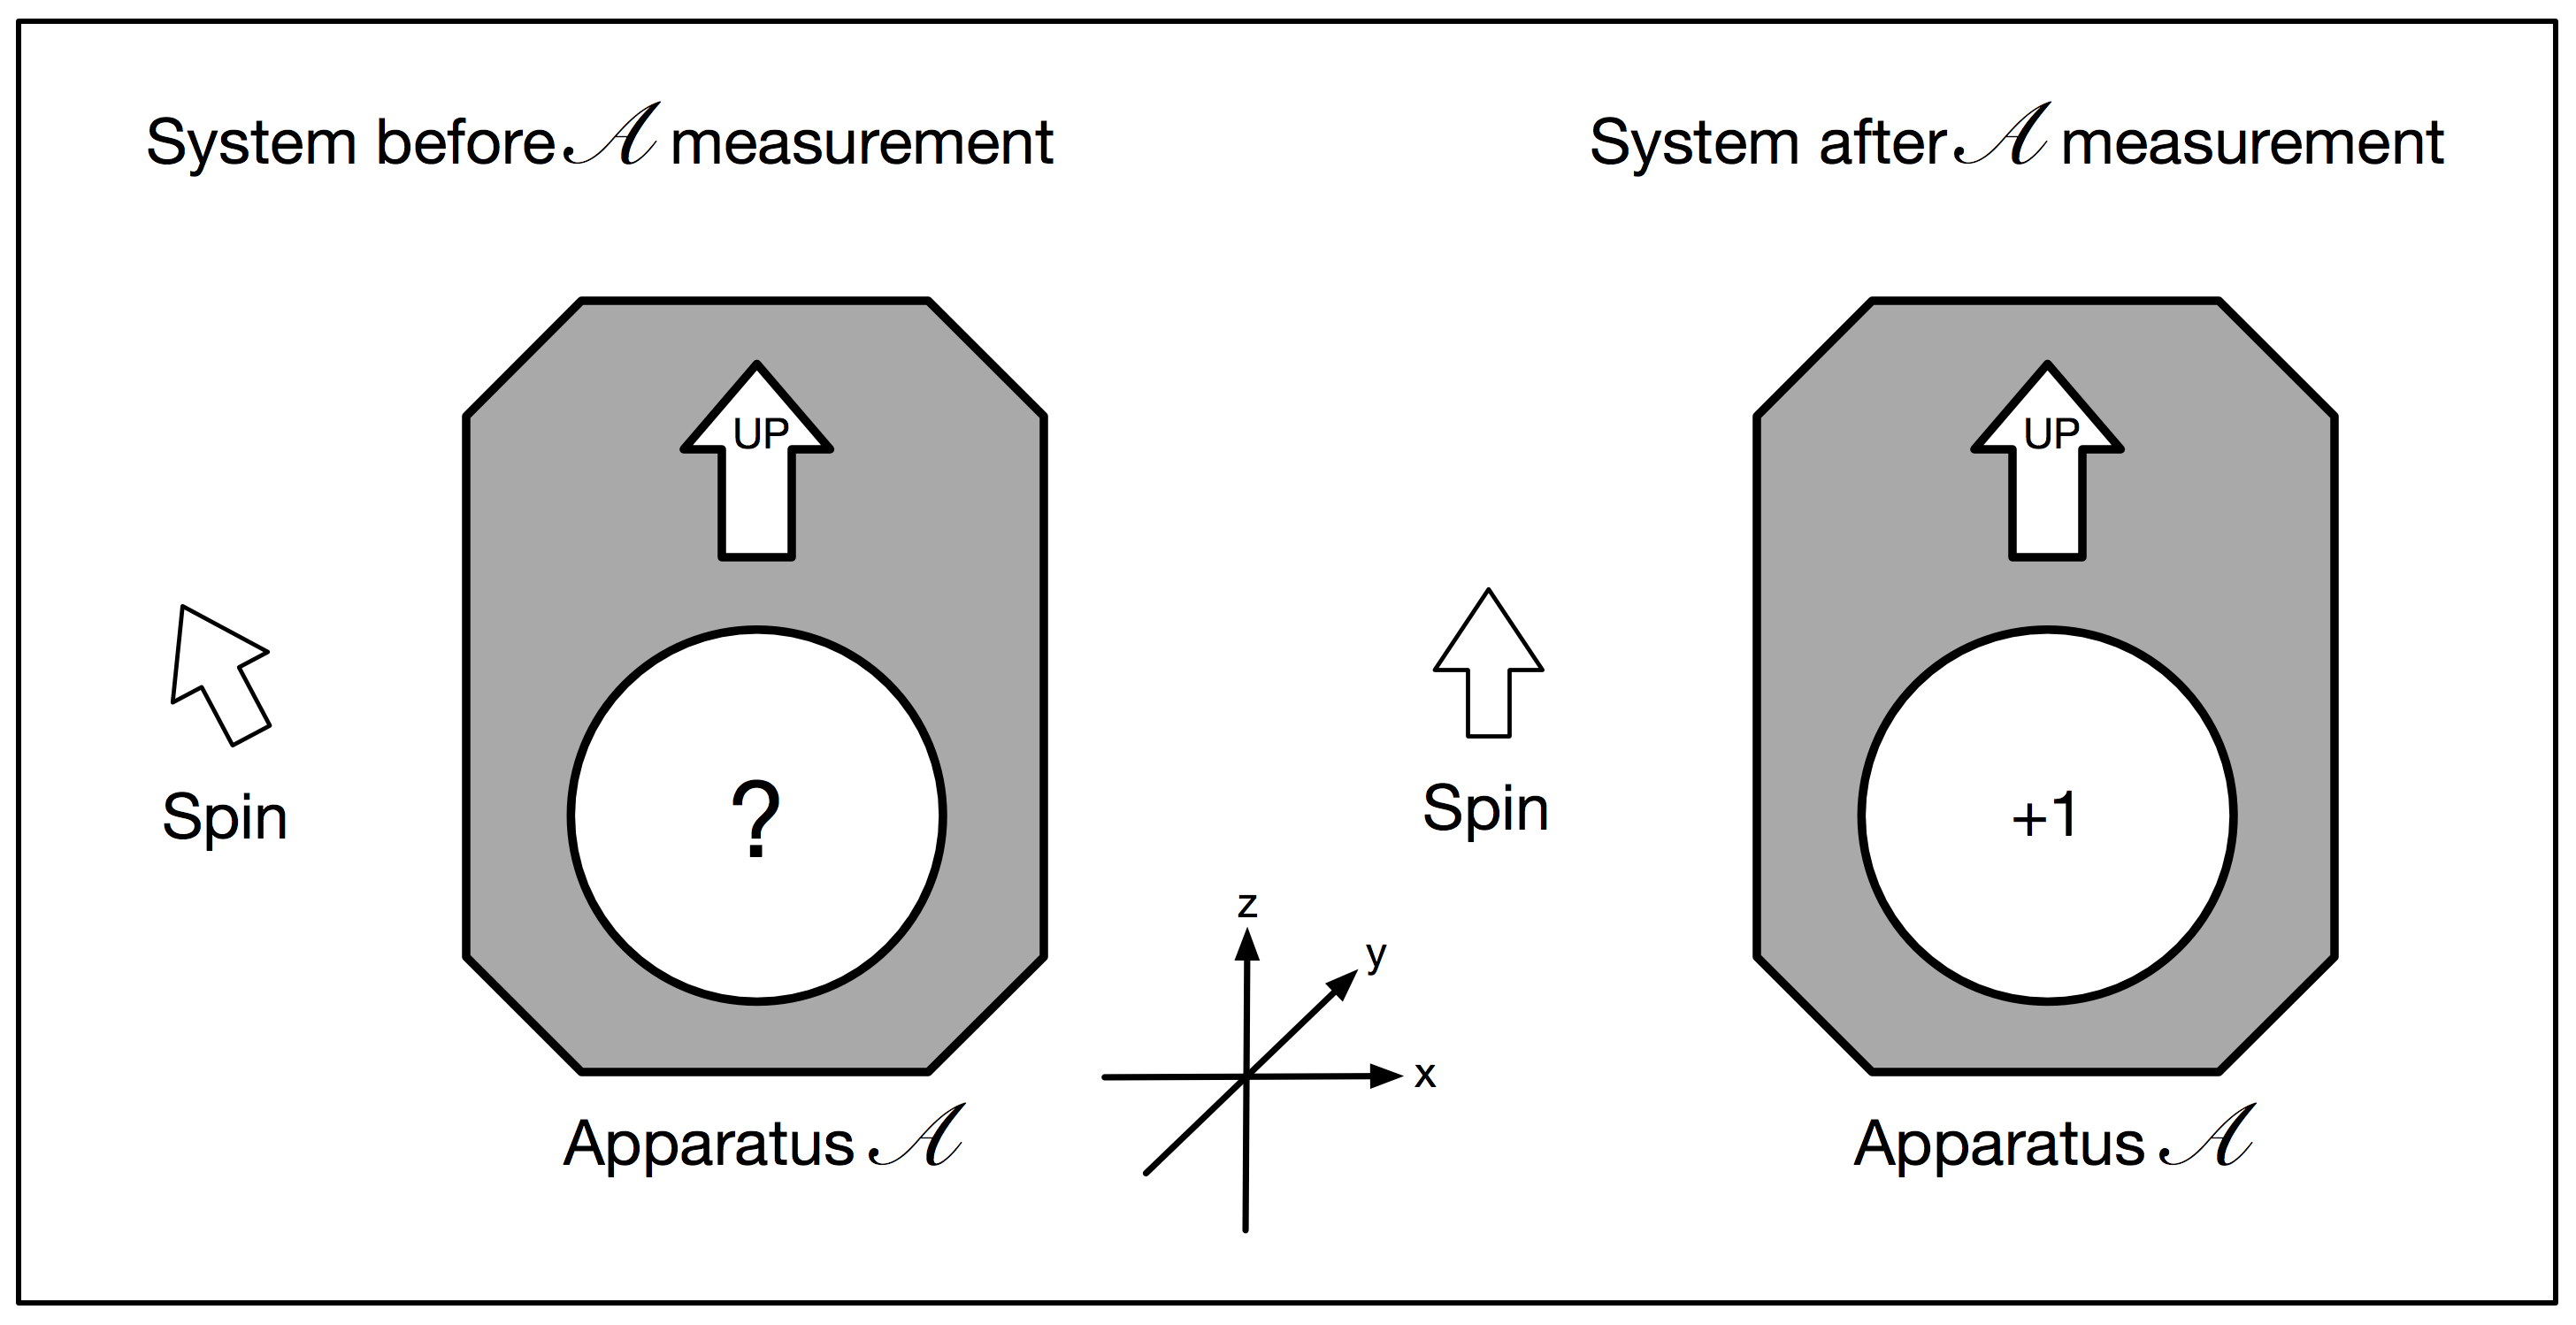
\includegraphics[width=4.5in]{images/spinExp1.png}
\caption{A first measurement.}
\label{fig:spinExp1}
\end{center}
\end{figure}

For the first experiment, the black box points along the $z$ axis, as shown in \autoref{fig:spinExp1}. Initially you don't have no knowledge of whether $\sigma = +1$ or $\sigma = -1$: the purpose of the experiment is to find out the value of $\sigma$.

Before the apparatus \textit{interacts} with the spin, the window is blank: after the measurements of $\sigma$, the question mark disappears and the window shows a $+1$ or a $-1$. Now that you measured $\sigma$, let's reset the apparatus to neutral and, without \textit{disturbing} the spin, measure $\sigma$ again.

Assuming the spin evolution law, you should get the same answer got after the first measurement: thus, the result $\sigma = +1$ will be followed by $\sigma = +1$, likewise for $\sigma = -1$. Further, this sequence of results will be true for any number of repetitions, allowing you to confirm the result of an experiment: in a sense, the first interaction with the apparatus $\mathcal{A}$ \textit{prepares} the system in one of the two states. Subsequent experiments \textit{confirm} that state. So far, there is no difference between classical and quantum physics: at least for now.

\subsubsection{Introducing some rotations}

\paragraph{} Let's do something new. After preparing the spin by measuring it with $\mathcal{A}$, turn the apparatus upside down and then measure $\sigma$ again, as shown in \autoref{fig:spinExp2}.

\begin{figure}[!htb]
\begin{center}
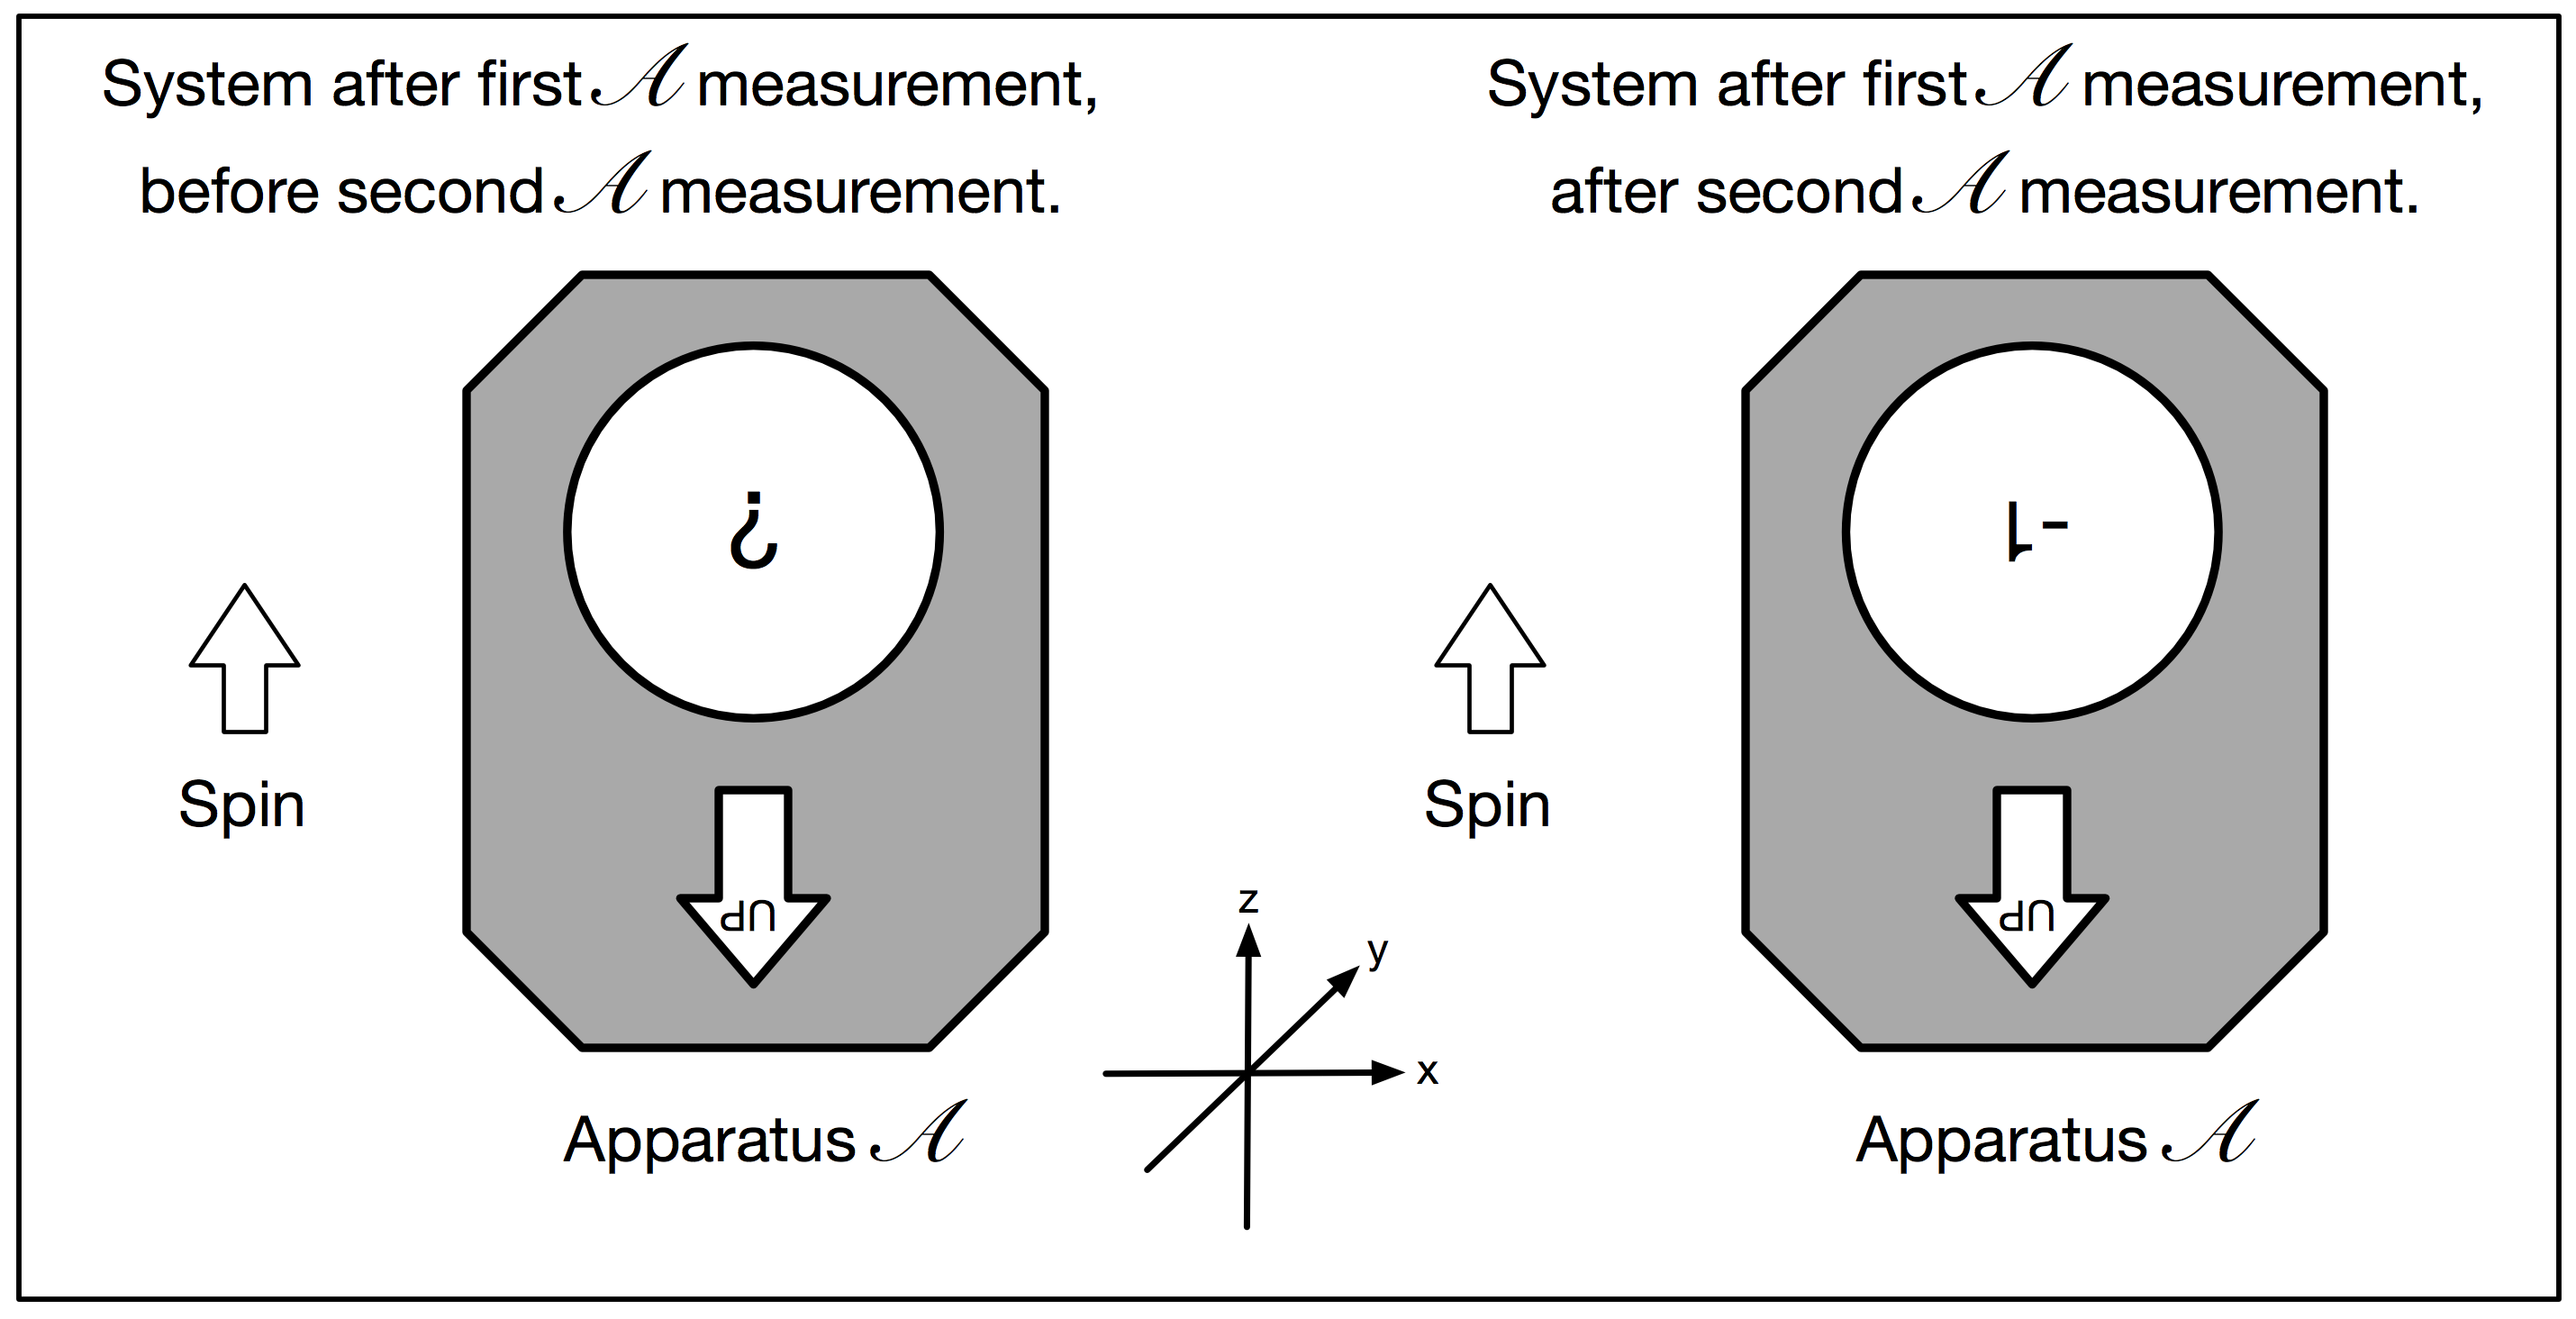
\includegraphics[width=4.55in]{images/spinExp2.png}
\caption{A second measurement: the spin is \textit{prepared} and then measured again with the apparatus rotated by 180 degree.}
\label{fig:spinExp2}
\end{center}
\end{figure}

What we find is that if you originally prepared $\sigma = +1$, the upside down apparatus records $\sigma = -1$. Similarly, if we originally prepared $\sigma = -1$, the upside down apparatus records $\sigma = +1$. In other words, turning the apparatus over \textit{interchanges} $\sigma = +1$ and $\sigma = -1$. From these results, you might conclude that $\sigma$ is a ``degree of freedom" that is associated with a sense of direction in space. 

For instance, if $\sigma$ were an oriented vector of some sort, then it would be natural to expect that turning the apparatus over would reverse the reading. A simple explanation is that the apparatus measures the componet of the vector along the axis embedded in the apparatus. The question is now: is this explanation correct for all configurations of spin and/or apparatus direction?

If you are convinced that the spin is a vector, you would naturally describe it by three components, or degree of freedom: $\sigma_z, \; \sigma_x, \; \sigma_y$. When the apparatus is upright along the $z$ axis, it is positioned to measure $\sigma_z$. 

So far, there is still no difference between classical physics and quantum physics. The difference only becomes apparent when you rotate the apparatus through an arbitrary angle, say $\frac{\pi}{2}$, or $\ang{90}$ degrees. The apparatus begins in the upright position, i.e. with the up-arrow along the $z$ axis. A spin is prepared with $\sigma = +1$. Next, the apparatus $\mathcal{A}$ is rotated so that the up-arrow points along the $x$ axis as shown in \autoref{fig:spinExp3}, and then make a measurement of what is presumably the $x$ component of the spin, $\sigma_x$.

\begin{figure}[!htb]
\begin{center}
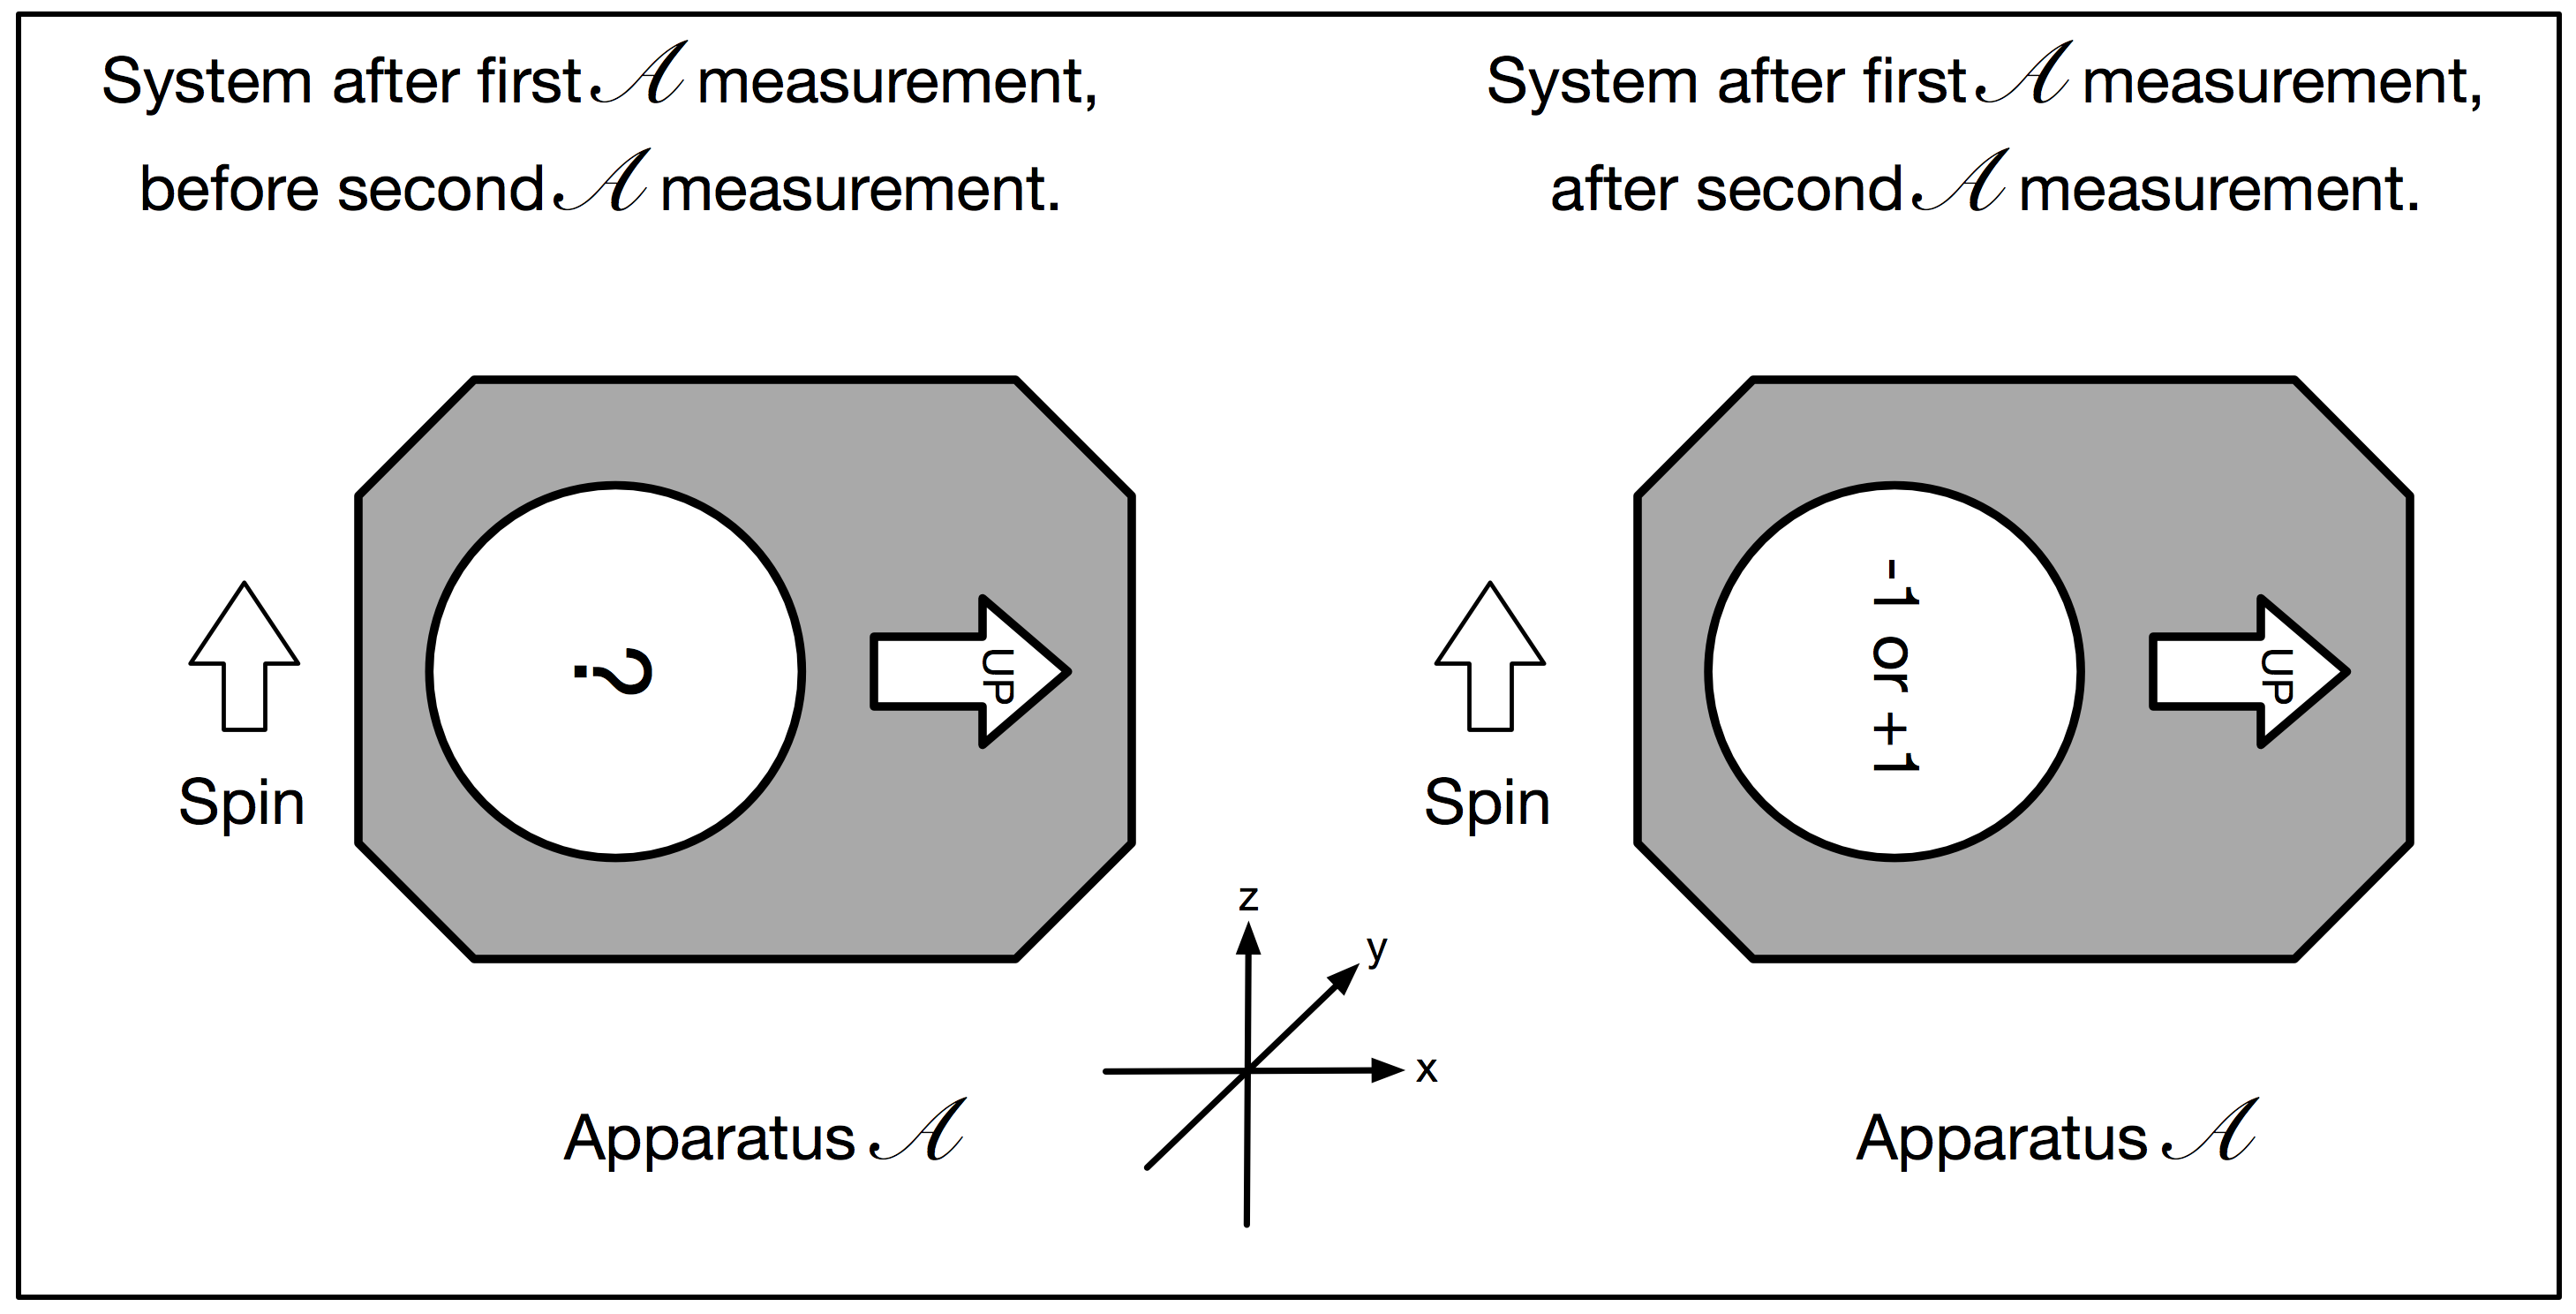
\includegraphics[width=4.55in]{images/spinExp3.png}
\caption{A third measurement over the x component of the spin.}
\label{fig:spinExp3}
\end{center}
\end{figure}

If $\sigma$ really represents the components of a vector along the up-arrow, one would expect to get zero. Why? Initially, we confirmed that $\sigma$ was directed along the $z$ axis, suggesting that its component along $x$ must be zero. However, after the $\sigma_x$ measurement, instead of giving $\sigma_x = 0$, the apparatus $\mathcal{A}$ gives either $\sigma_x = +1$ or $\sigma_x = -1$. Furhter, no matter which way $\mathcal{A}$ is oriented, it refuses to give any answer other than $\sigma = \pm1$.

Nevertheless, we do find something interesting. Suppose we repeat the operation many times, each time following the same procedure, that is:

\begin{itemize}
    \item Beginning with $\mathcal{A}$ along the $z$ axis, prepare $\sigma = +1$.
    \item Rotate the apparatus so that it is oriented along the $x$ axis.
    \item Measure $\sigma$.
\end{itemize}

\paragraph{An important difference} The repeated experiment spits out a random series of plus-ones and minus-ones. Determinism has broken down, but in a particular way. if we do many repetitions, we will find that the numbers of $\sigma = +1$ events and $\sigma = -1$ events are statistically equal. In other words, the average value of $\sigma$ = 0. Instead of the classical result - namely, that the component of $\sigma$ along the $x$ axis is zero - we find that the \textit{average of these repeated measurements} is zero. 

If the spin is a vector, it is a very peculiar one indeed.

\subsubsection{A strange vector}

\paragraph{} Let's do the whole thing over again, but instead of rotating $\mathcal{A}$ to lie on the $x$ axis, rotate it to an arbitrary direction along the unit vector $n$. Classically, if $\sigma$ were a vector, you would expect the result of the experiment to be the component of $\sigma$ along the $n$ axis. If $n$ lies at an angle $\theta$ with respect to $z$, the classical answer would be $\sigma = cos(\theta)$. But as you might guess, each time we do the experiment we get $\sigma = +1$ or $\sigma = -1$. However, the result is statistically biased so that the average value is $cos(\theta)$.

\begin{figure}[!htb]
\begin{center}
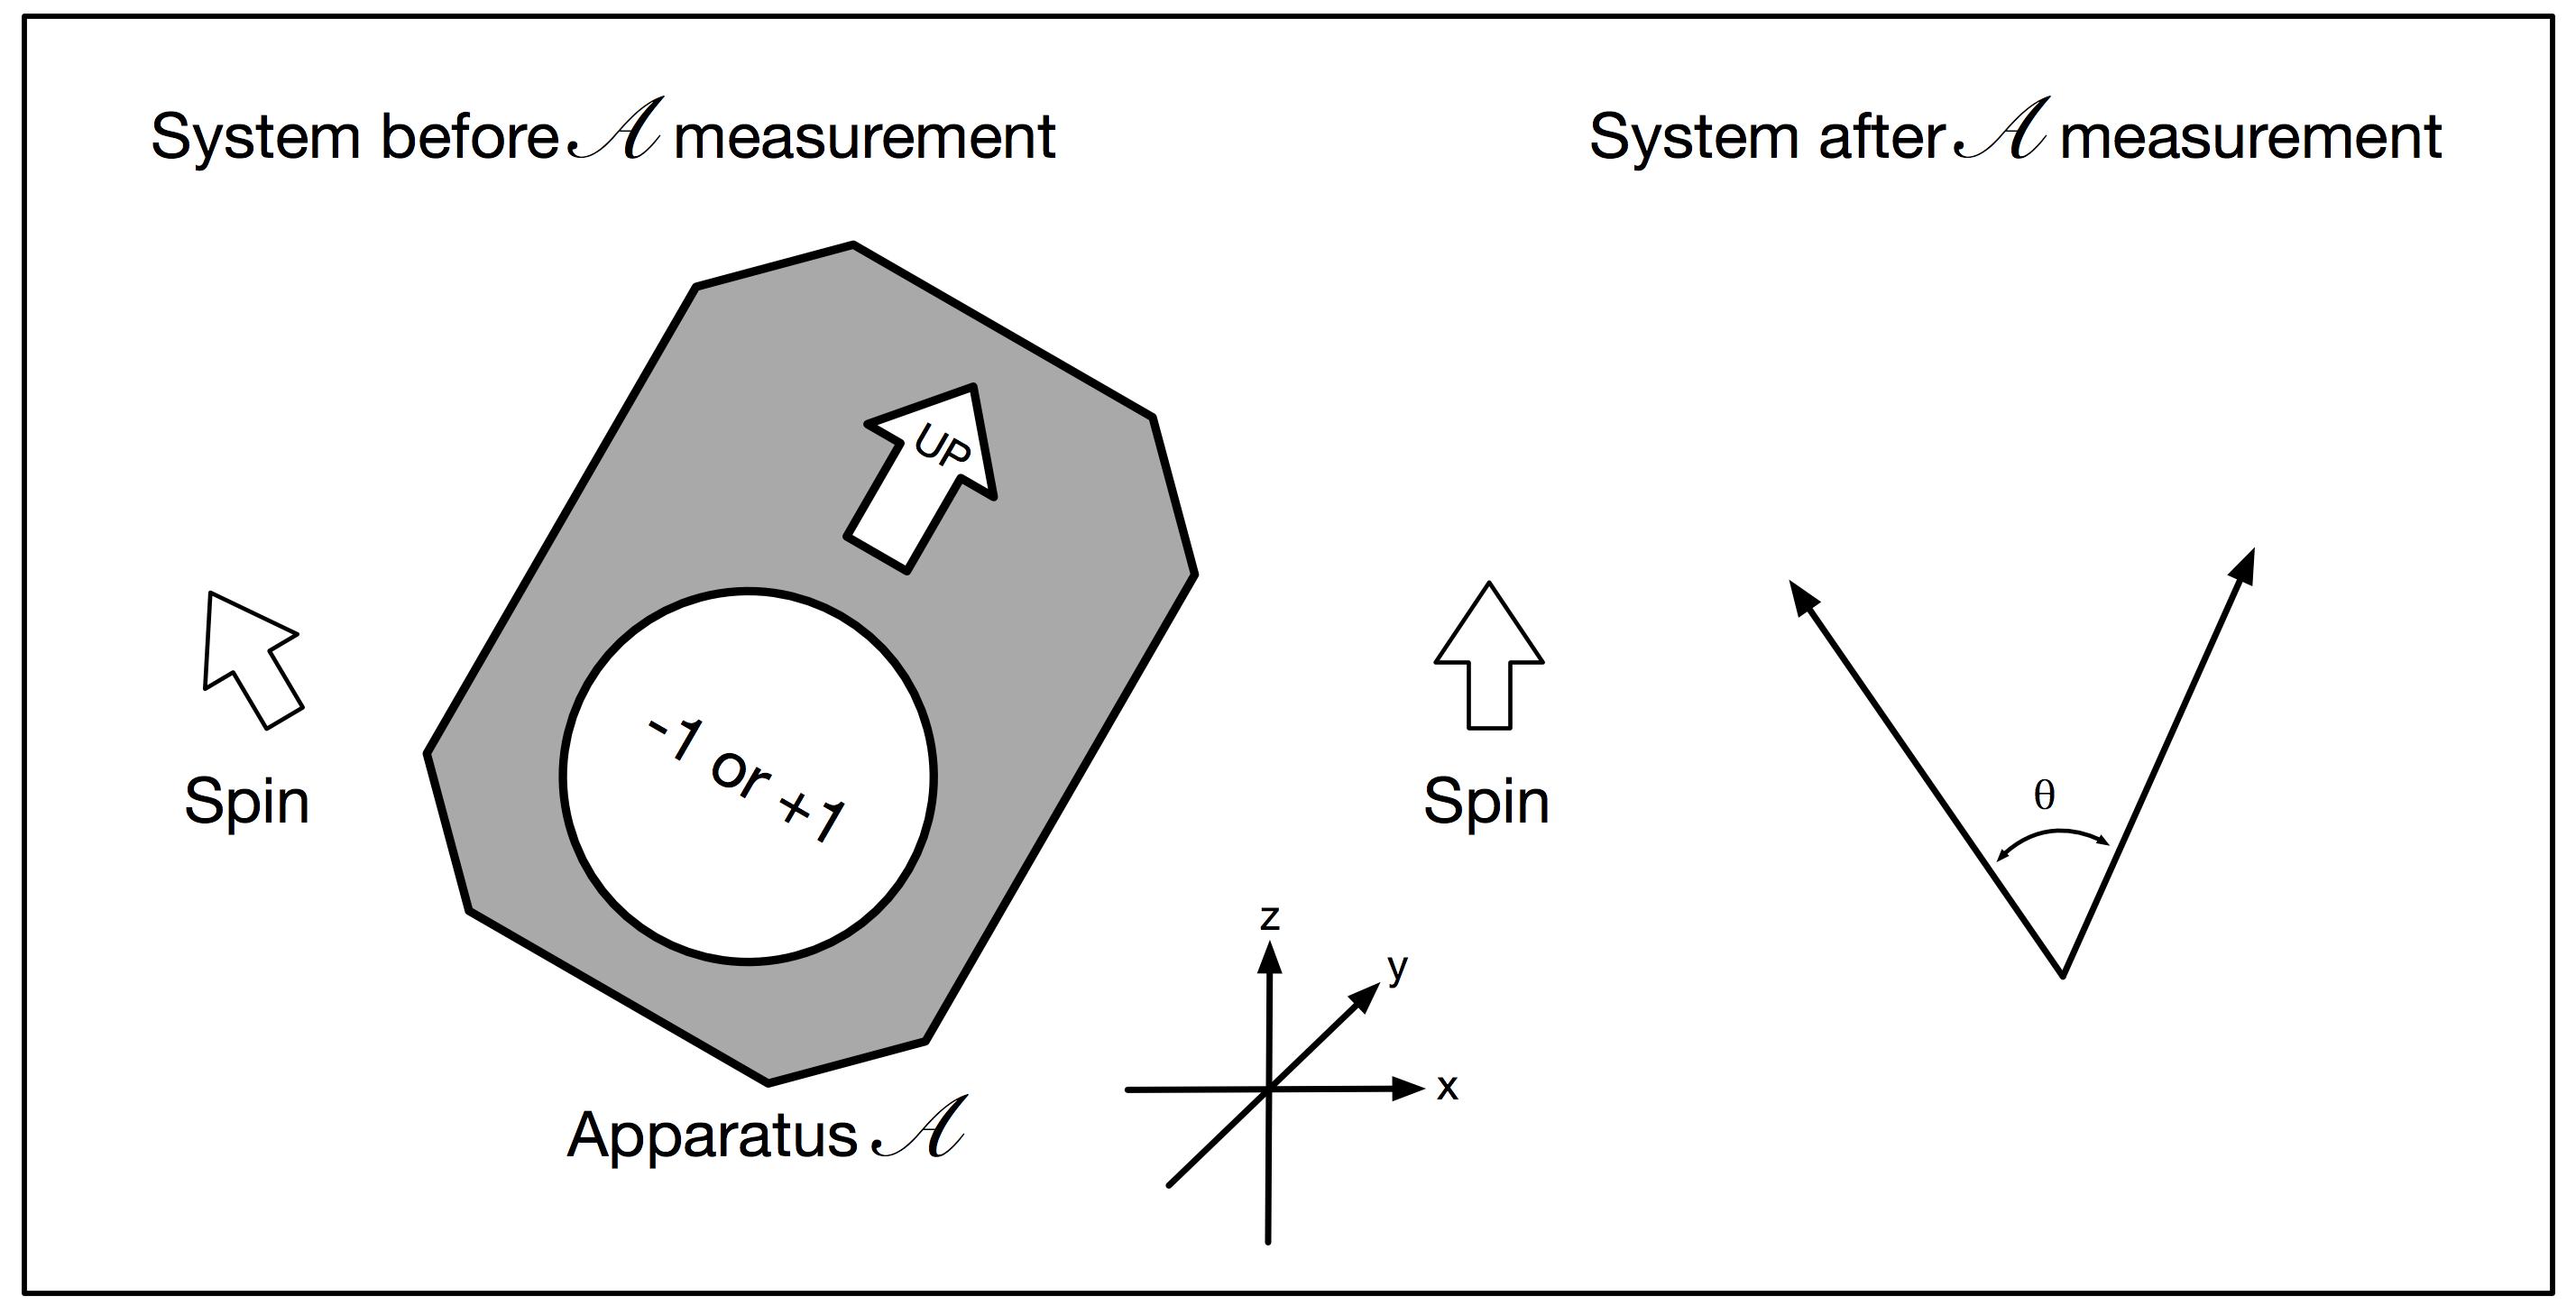
\includegraphics[width=4.55in]{images/spinExp4.png}
\caption{An arbitrary rotation and measurement of the spin component.}
\label{fig:spinExp4}
\end{center}
\end{figure}

The situation is of course more general. We did not have to start with $\mathcal{A}$ oriented along $z$. Pick any direction $m$ and start with the up-arrow pointing along $m$. Prepare a spin so that the apparatus reads $+1$. Then, without disturbing the spin, rotate the apparatus to the direction $n$, as shown in \autoref{fig:spinExp4}. A new experiment on the same spin will give random results $\pm 1$, but with an average value equal to the cosine of the angle between $n$ and $m$. In other words, the average will be $n \cdot m$.

The quantum mechanical notation for the statistical average of a quantity $Q$ is Dirac's bracket notation\footnote{The Dirac notation is foundamental in quantum mechanics: more on that will be said in the mathematical recall.} $\langle Q\rangle$. You may summarize the results of the experimental investigation as follows: if you begin with $\mathcal{A}$ oriented along $m$ and confirm that $\sigma = +1$, then subsequent measurements with $\mathcal{A}$ oriented along $n$ gives the statistical result
$$\langle\sigma\rangle = n \cdot m$$

What I'm saying is that quantum mechanical systems are not deterministic - the results of experiments can be statistically random - but if we repeat an experiment many times, average quantities can follow the expectations of classical physics, at least up to a certain point.

\subsection{A different kind of logic}

\paragraph{} Every experiment involves an outside system - an apparatus that must interact with the system in order to record a result: in that sense, every experiment is \textit{invasive}. In fact, each first lessons of physics starts - at least, should - by removing from students the idea of obtaining any kind of absolute precise measure of a system or one of its characteristics. This is impossible, even in classical physics. However, an ideal measuring apparatus has often a vanishingly small effect on the system it is measuring.

\subsubsection{Quantum mechanics: the effect of interactions}

\paragraph{} In quantum mechanics, the situation if foundamentally different. Any interaction that is strong enough to measure some aspect of a system is \textit{necessarily strong enough} to disrupt some other aspect of the same system. Thus, you can learn nothing about a quantum system without changing something else.

This should be evident in the example involving $\mathcal{A}$ and $\sigma$. Suppose you begin with $\sigma = +1$ along the $z$ axis. If you measure $\sigma$ again with $\mathcal{A}$ oriented along $x$, you will confirm the previous value. You can do this over and over without changing the result. But consider this possibility: between subsequent measurements along the $x$ axis, you turn $\mathcal{A}$ through $\ang{90}$ degrees, make an intermediate measurement, and turn it back to its original direction. Will a subsequent measurement along the $z$ axis confirm the original measurement?

The answer is no. The intermediate measurement along the $x$ axis will leave the spin in a completely random configuration, as far as the next measurement is done. There is no way to make the intermediate determination of the spin without completely disrupting the final measurement. One might say that measuring one component of the spin destroys the information about another component. In fact, one simply cannot \textit{simultaneously} know the components of the spin along two different axes - at least, not in a reproducible way in any case.

This is to say that there is something fundamentally different about the state of a quantum system and the state of a classical system.

\subsubsection{Measurements order matters}

\paragraph{} The space of states of a classical system is a mathematical set. If the system is a coin, the space state is $\{H,T\}$. As in classical boolean logic, also in set theory there is, in a sense, the concept of ``nothing other than true or false is allowed": this concept is expressed by the subset. Roughly, we can say that a proposition is true if it is true \textit{for each elements it contains} in its subset and false for each other elements. What does it mean? For instance, the sentence ``the die shows an odd-numbered face" about the system ``die" is \textit{true} if - for each elements of its subset $\{1,3,5\}$ - is \textit{true} and \textit{false} for each others. There are no other possibilieties\footnote{Just kidding: have a look at default logic and non-monotonic reasoning.}. Further, propositions could be mixed with logical operators like \texttt{OR}, \texttt{AND} and \texttt{NOT}.

Let's return to the simple quantum system consisting of a single spin and the various propositions whose truth we could test using the apparatus $\mathcal{A}$. Consider the following sentences:
\begin{itemize}
    \item A: the $z$ component of the spin is $+1$;
    \item B: The $x$ component of the spin is $+1$;
    \item $\neg$A: The $z$ component of the spin is $-1$;
    \item A \texttt{OR} B: The $z$ component of the spin is $+1$ or the $x$ component of the spin is $+1$;
    \item A \texttt{AND} B: The $z$ component of the spin is $+1$ or the $x$ component of the spin is $+1$;
\end{itemize}

Imagine we have to test the truth of the $4$-th sentence: we can use the apparatus $\mathcal{A}$, measure $\sigma_z$ and, if it's equal to $-1$, go ahead with measurement of $\sigma_x$.

What happens if we change the order of measurements in a classical system - a one in which the spin is a normal vector? You will obtain the same result from both the measurements. However, we don't know yet how a spin works, but we already verified that is not a definetily not classical system.

Let's do it in the quantum way: you measure $\sigma_z$, you discover $\sigma_z = +1$. A \texttt{OR} B is true. Now, suppose you want to test also $\sigma_x$: the answer is unpredictable. This is not a problem, because the sentence A \texttt{OR} B remains true.

Now, let's try to repeat the measure inverting the order and testing B \texttt{OR} A. First, the measure of $\sigma_x$ is random because the first measure of $z$ (in A \texttt{OR} B experiment) set the $\sigma_z = +1$. So, let suppose the result is $\sigma_x = +1$: than, B \texttt{OR} A is true. However, if the result is $\sigma_x = -1$, then it means that the spin is oriented along the $-x$ direction. And this is strange, because the spin is no longer in its original state $\sigma_z = +1$, but in a new state that is either $\sigma_x = +1$ or $\sigma_x = -1$.

Now, test the second half of B \texttt{OR} A: in other words, rotate the apparatus $\mathcal{A}$ and measure $\sigma_z$. According to quantum mechanics, the result will be randomly $\pm 1$: this means that there is a $25\%$ probability that the experiment produces $\sigma_x = -1$ and $\sigma_z = -1$. In other words, with a probability equal to $1/4$ we find that B \texttt{OR} A is false. And this occurs despite the fact the there is unknown agent that originally made sure that $\sigma_z = +1$ (see first experiment).

The point is that the inclusive \texttt{OR} is not \textit{symmetric}: the truth of A \texttt{OR} B may depend on the order in which you confirm the two propositions.

\subsubsection{The uncertainty principle}

\paragraph{} At this point, you probably recognize that the result of the experiments we conducted are due to the famous uncertainty principle: this doesn't apply only to position and momentum (or velocity), but it applies to many pairs of measurable quantities. In the case of the spin, it applies to propositions involving two different components of $\sigma$. In the case of position and momentum, the two propositions we might consider are:
\begin{itemize}
    \item A certain particle has position $z$;
    \item The same particle has momentum $p$;    
\end{itemize}

From these, we can form the two composite propositions
\begin{itemize}
    \item The particle has position $x$ and the particle has momentum $p$;
    \item The particle has position $x$ or the particle has momentum $p$;
\end{itemize}

In quantum mechanics, the first of these propositions is completly meaningless (not even wrong), and the second one means something quite different from someone could think normally. It all comes down to a deep logical difference between the classical and quantum concepts of the state of a system. But explaining quantum concepts require some mathematics concept first: to make these notes more useful for other, I collected all the maths needed to understand the concept exposed in the subsequent sections in a unique section, the next one. Every time I will refer to a particular mathematical properties, theorems, axioms, and so on, I will insert a reference back to the point in which it is discussed.

\newpage

\section{Mathematical Interpretation}

\paragraph{} A qubit is described as an \textit{abstract mathematical object} that enjoys certain particular properties. The physical nature of this object will be clarified later by observing the correspondence between the properties of a qubit with those of any two-state quantum system: some features of this system were already discussed in the previous example (see \autoref{subsec:spinExample}). 
In this section, I will introduce - as clearly as possible - some definitions and notations needed to understand the mathematical model of the qubit, the operations you can do on it and the laws the govern the quantum world: many of the following exposed concepts are fundamental for understanding the physical phenomena underlying quantum computation. 

My advice is to spend all the time necessary to understand these basic and easy-to-understand concepts, and to return to this section whenever you don't remember somethings. Enjoy the reading!

\subsection{Vectorial Space}

\paragraph{} The \textbf{two-dimensional real vector space} ${\mathbb{R}}^2$ is the set of column vectors
\begin{equation}
v = \binom{a}{b}
\label{eq:vectorInR2}
\end{equation}

where $a, b \in \mathbb{R}$ are real numbers. 

\paragraph{} The \textbf{norm} of $v$ is given by
\begin{equation}
|v| = \sqrt{a^2 + b^2}
\label{eq:vectorNormInR2}
\end{equation}

\paragraph{} The \textbf{transposed} of $v$ is the vector line
\begin{equation}
v^T = (a, b)
\label{eq:vectorTransposedInR2}
\end{equation}

\paragraph{} The \textbf{scalar product} - also called \textbf{inner} or \textbf{internal} product - of two vectors
\begin{equation*}
v_1 = \binom{a_1}{b_1}, v_2 = \binom{a_2}{b_2}
\end{equation*}

is given by 
\begin{equation}
v_1 \cdot v_2 \stackrel{\text{def}}{\equiv} v_1^Tv_2 = (a_1, b_1) \binom{a_2}{b_2} = a_1 a_2 + b_1 b_2 = \norm{v_1}\norm{v_2}cos{\theta}
\label{eq:vectorScalarProductInR2}
\end{equation}

where ${\theta}$ is the angle between $v_1$ and $v_2$.

\paragraph{} Two vectors $v_1, v_2$ are \textbf{orthogonal} if $v_1 \cdot v_2 = 0$.

\paragraph{} The vectors ${v_i \in {\mathbb{R}} \; | \; i = 1, 2,\ldots k}$ are \textbf{linearly independent} if
\begin{equation}
a_1v_1 + a_2v_2 + \ldots + a_kv_k = 0, \; \; a_i \in {\mathbb{R}}
\label{eq:vectorLinearIndipendentInR2}
\end{equation}

This implies that $a_i = 0$ for each $i = 1, 2, \ldots, k$. Otherwise they are called \textbf{linearly dependent}.

\subsection{Orthonormal Bases} 

\paragraph{} A \textbf{basis} of ${\mathbb{R}}^2$ is any set of linearly independent vectors such that any other vector in ${\mathbb{R}}^2$ can be expressed as a linear combination of the vectors in the set. Each pair/set of $v_1$ and $v_2$ linearly independent vectors form a base for ${\mathbb{R}}^2$/${\mathbb{R}}^n$.

\paragraph{} Further, $v_1$ and $v_2$ form an \textbf{orthonormal basis} for ${\mathbb{R}}^2$ if $\norm{v_1} = \norm{v_2} = 1$ \textbf{and} $v_1 \cdot v_2 = 0$.
Consequently, the two vectors
\begin{equation}
\binom{1}{0} \; \; \; \binom{0}{1}
\label{eq:standardBaseInR2}
\end{equation}

form an orthonormal basis for ${\mathbb{R}}^2$ called the \textbf{standard base} of ${\mathbb{R}}^2$.

\paragraph{} In ${\mathbb{R}}^2$ and ${\mathbb{R}}^3$, the most common basis are the 2/3 unit vectors that point along the $x, y$ and $z$ axes. Obviously, there is nothing special about this particolar axis: as long as the basis vectors are of unit length and are mutually orthogonal, they form an orthonormal basis.

The same principle is true for complex vector spaces. One can begin with any normalized vector and then look for a second, orthogonal to the first. If you find one, then the space is at least two-dimensional. Then look for a third, fourth, and so on. Eventually, you may run out of new directions and there will not be any more orthognal vectors is the dimension of the space.

The point is: the maximum number of mutually orthogonal vectors is the dimension of the space. For column vectors, the dimensions is simply the number of entries in the column.

\subparagraph{Gram-Schmidt}
\label{subpar:gramschmidt}
It is always possible to transform any base for a $V$ vector space into an orthonormal base. The method for doing so is called the Gram-Schmidt procedure: thanks to this procedure we can assume that the bases we will consider from now on are always orthonormal.\from{Matteo}{Eventually extend this with explanation by Susskind.}

\paragraph{Exercise} Look exercises number 1 in \autoref{exs}.

\paragraph{} Before going on with the qubits definitions, we first introduce the definition of a complex numbers and some basic properties defined on them.

\subsection{Complex Numbers}

\paragraph{} A \textbf{complex number} $z$ is a number expressed in the form
\begin{equation}
z = a + ib
\label{eq:complexNumber}
\end{equation}

where $a, b \in {\mathbb{R}}$ are real numbers and $i = \sqrt{-1}$ is the imaginary unit. For further notation, we call $a = Re(z)$ the real part of $z$ and $b = Im(z)$ the imaginary part.

\paragraph{} The \textbf{norm} or \textbf{module} of a complex number $z \in \mathbb{C}$ is 
\begin{equation}
|z| = \sqrt{a^2 + b^2}
\label{eq:complexNumberNorm}
\end{equation}

\paragraph{} Each complex number has a sort of \textit{dual}, called \textbf{complex conjugate}: given a complex number $z \in \mathbb{C}$, its conjugate is
\begin{equation}
z^* = a - ib
\label{eq:complexNumberConjugate}
\end{equation}

\paragraph{} The \textbf{two-dimensional complex vector space} ${\mathbb{C}}^2$ is the set of column vectors of the form
\begin{equation}
w = \binom{\alpha}{\beta}
\label{eq:twoDimensionalComplexVectorSpace}
\end{equation}

with ${\alpha}, {\beta} \in {\mathbb{C}}^2$.

\paragraph{} The \textbf{norm} of the two-dimensional complex vector $w \in {\mathbb{C}}^2$ is given by
\begin{equation}
\norm{w} = \sqrt{|\alpha|^2 + |\beta|^2}
\label{eq:complexVectorNorm}
\end{equation}

where $|z|$ is the module of the complex number $z$. So, given $\alpha  = a_1 + ib_1$ and $\beta  = a_2 + ib_2$, then the norm of the vector $w^T = (\alpha, \beta)$ is given by
\begin{equation*}
\norm{w} = \sqrt{|\alpha|^2 + |\beta|^2} = \sqrt{\left|\sqrt{a_1^2 + b_1^2}\right|^2 + \left|\sqrt{a_2^2 + b_2^2}\right|^2} = \sqrt{a_1^2 + b_1^2 + a_2^2 + b_2^2}
\end{equation*}

\paragraph{} The \textbf{complex conjugate} of the two-dimensional complex vector $w = \binom{\alpha}{\beta} \in {\mathbb{C}}^2$ is the linear vector
\begin{equation}
w^\dagger = {(w^{T})}^{*} = {(w^{*})}^{T} = (\alpha^*, \beta^*)
\label{eq:twoDimensionalComplexVectorConjugate}
\end{equation}

with $(\alpha^*, \beta^*)$ the two \textbf{complex conjugate} of $\alpha$ and $\beta$.

\paragraph{} The \textbf{scalar product} - also called \textbf{inner} or \textbf{internal} product - of two complex vectors
$$w_1 = \binom{\alpha_1}{\beta_1} \; \; \; w_2 = \binom{\alpha_2}{\beta_2}$$

is defined as
\begin{equation}
w_1 \cdot w_2 \stackrel{\text{def}}{=} w_1^\dagger w_2 = (\alpha_1^*, \beta_1^*) \binom{\alpha_2}{\beta_2} = \alpha_1^* \alpha_2 + \beta_1^*\beta_2
\label{eq:complexVectorScalarProductInC2}
\end{equation}

Remember that - given $z_1 = a + ib$ and $z_2 = c + id$ ($z_1, z_2 \in {\mathbb{C}}^2$), the product $z_1 z_2$ is
\begin{equation*}
\begin{split}
z_1z_2 & = (a + ib) (c + id) = ac + aid + ibc + ibid = \\
 & = ac + aid + ibc - bd = ac - bd + i(ad + bc) \\
\end{split}
\end{equation*}

\paragraph{} The definitions of linear, base, and orthonormal independence are similar to those for ${\mathbb{R}}^2$.
Consequently, the two vectors
\begin{equation}
\binom{1}{0} \; \; \; \binom{0}{1}
\label{eq:canonicalBaseInC2}
\end{equation}

form an orthonormal basis for ${\mathbb{C}}^2$ called \textbf{canonical basis}. 

\subsection{The Dirac notation}
\label{diracNotation}
\paragraph{} To represent the elements of a complex vector space it is convenient to use a notation called \textbf{Dirac notation} from the name of the famous English physicist, pioneer of quantum theory, who introduced it: the Dirac notation represents the standard notation in quantum mechanics.

According to this notation, $|v\rangle$ or \textbf{ket} indicates a generic element of the vector space ${\mathbb{C}}^2$.

As shown before, the complex numbers have a \textit{dual} version in the form of complex conjugate numbers. In the same way, a complex vector space has a dual version that is essentialy the complex conjugate vector space. Thus, for every ket-vector $|v\rangle$ there is a \textbf{bra} vector denoted by $\langle v|$ belonging to the complex conjugate of the vector space. There are some simple properties to remember between bras and kets.

Suppose that $\langle v$ is the bra corresponding to the ket $|v\rangle$, and $\langle w$ is the bra corresponding to the ket $|w\rangle$. Then the bra corresponding to
\begin{equation*}
|v\rangle + |w\rangle
\end{equation*}
is
\begin{equation*}
\langle v| + \langle w|
\end{equation*}

If $z$ is a complex number, then the bra corresponding to 
\begin{equation*}
z|v\rangle
\end{equation*}
is
\begin{equation*}
\langle v|z^*
\end{equation*}

In the concrete example, where \textit{kets} are represented by column vectors, the dual \textit{bras} are represented by row vectors, with the entries being drawn from the complex conjugate numbers. Thus, if the ket $|a\rangle$ is represented by the column
\begin{equation*}
\begin{pmatrix}
    \alpha_1\\
    \vdots\\
    \alpha_d
\end{pmatrix}
\end{equation*}
then the corresponding bra $\langle a|$ is represented by the row
\begin{equation}
(\alpha_1, \alpha_2, \ldots, \alpha_d)
\label{eq:braOfKetDefinition}
\end{equation}

% If $|v\rangle$ or \textbf{ket} indicates a generic element of the vector space, $|i\rangle$ indicates the $i_{th}$ element of the canonical orthonormal basis. If $|v\rangle = \sum\limits_{i}{\alpha_i|i\rangle}$ e $|w\rangle = \sum\limits_{i}{\beta_i|i\rangle}$, then their scalar product 
% $$(\alpha_1, \alpha_2, \ldots, \alpha_d) \; \begin{pmatrix}
%     \beta_1\\
%     \vdots\\
%     \beta_d
% \end{pmatrix}
% $$

% is indicated with $\langle v | w\rangle$. The $\langle v | w\rangle$ form a \textbf{braket}.

% More in general, in the concret example where kets are represented by column vectors, the dual bras are represented by row vectors: the bras are the complex conjugate of their respective kets.

% \from{Matteo}{Integrate with Susskind and Friedman lesson.}

% The definition implies that each internal product satisfies the following property:
% $$\sum\limits_{i}(a_i|w_i\rangle, |v\rangle) = \sum\limits_{i}a_i^{*}(|w_i\rangle, |v\rangle)$$

% In Dirac's notation, the internal product of vector $|v\rangle$ with vector $|w\rangle$ is denoted by $\langle v|w\rangle$. Using the internal product, you can define the norm of a vector as
% $$||v|| = \sqrt{\langle v\rangle}$$

The usefulness of this notation will be particularly evident to study quantum measurement and in particular projection operators.

\subsection{Internal product}

\paragraph{} The formal definition of a internal product is the following: given a vector space $V$, a function $(\cdot, \cdot): V \times V \mapsto \mathbb{C}$ is called internal or inner or scalar product if it meets the following requirements:
\begin{itemize}
    \item $(|v\rangle, |v\rangle) \geq 0$
    \item $(|v\rangle, |v\rangle) = 0 \leftrightarrow v = 0$
    \item $(|v\rangle, |w\rangle) = (|w\rangle, |v\rangle)*$
    \item $(|v\rangle, \sum\nolimits_{i}a_i|w_i\rangle) = \sum\nolimits_{i}a_i(|v\rangle, |w_i\rangle)$
\end{itemize}

From a practical point of view, the internal or inner or scalar product is the dot product analogous operation between bras and kets. In fact, the inner product is always the product of a bra and a ket and it is written this way:
$$\langle B|A\rangle$$

In the concrete representation of bras and kets by row and column vectors, the inner product is defined in terms of components:
$$\langle B|A\rangle = (\beta_1^*, \beta_2^*)\binom{\alpha_1}{\alpha_2} = \beta_1^*\alpha_1 + \beta_2^*+\alpha_2$$

The rule to compute inner product is essentially the same as for dot products: add the products of corresponding components of the vectors whose inner product is being calculated. The result of the inner product operation is a complex number. The axioms for inner product are not too hard to guess:
\begin{itemize}
    \item It is linear, so $\langle C| \{|A\rangle + |B\rangle\} = \langle C|A\rangle + \langle C|B\rangle$
    \item Changing bras and kets corresponds to complex conjugation, so
    $$\langle B|A\rangle = \langle A|B\rangle^*$$
\end{itemize}

The second could no seems so obvious, but it's easy to verify. Let be $\langle B| = (\beta_1^*, \beta_2^*)$ and $|A\rangle = \binom{\alpha_1}{\alpha_2}$. Thus, the inner product between them is $\beta_1^*\alpha_1 + \beta_2^*\alpha_2$. 

Now, consider the corresponding ket of the bra $\langle B|$ and bra of the ket $|A\rangle$: so, $|B\rangle = \binom{\beta_1}{ \beta_2}$ and $\langle A| = (\alpha_1*, \alpha_2*)$. Thus, the inner product between them is $\alpha_1^*\beta_1 + \alpha_2^*\beta_2$.

Let's define $\alpha_i = x_i \pm iy_i$ (plus or minus if you are considering the conjugate or not) and $\beta_i = z_i \pm iw_i$. Then
\begin{equation*}
\begin{split}
\beta_1^*\alpha_1 + \beta_2^*\alpha_2 & = (z_1 - iw_1)(x_1 + iy_1) + (z_2 - iw_2)(x_2 + iy_2) = \\
 & = z_1x_1 + iz_1y_1 -iw_1x_1 + w_1y_1 + \\
 & + z_2x_2 + iz_2y_2 -iw_2x_2 + w_2y_2 \\
 & = (z_2x_2 + w_2y_2) + i(z_2y_2 - w_2x_2) \\
 & \ \\
\alpha_1^*\beta_1 + \alpha_2^*\beta_2 & = (x_1 - iy_1)(z_1 + iw_1) + (x_2 - iy_2)(z_2 + iw_2) = \\
 & = x_1z_1 + ix_1w_1 -iy_1z_1 + y_1w_1 + \\
 & + x_2z_2 + ix_2w_2 -iy_2z_2 + y_2w_2 + \\
 & = (z_2x_2 + w_2y_2) - i(z_2y_2 - w_2x_2) \\
\end{split}
\end{equation*}

To make equal the two expression, you have to compute the conjugate of the second. So, $\langle B|A\rangle = \langle A|B\rangle^*$. Q.E.D.

\paragraph{} A \textit{normalized vector} is a vector such that the inner product with itself is $1$, so a normalized vector is $\langle A|A\rangle = 1$. For ordinary vectors, the term \textit{normalized} is usually replaced with \textit{unit vector}.

\paragraph{} Since two vectors are orthogonal if their inner product is equal to $0$, then the two vectors in the example before are orthogonal if $\langle B|A\rangle = 0$. This is the same of saying that two real vector are orthogonal if their dot product is zero.

\subsection{Hilbert spaces}

\paragraph{} The ${\mathbb{C}}^2$ vector space with its scalar product is called the two-dimensional \textbf{Hilbert space}. More formally, a Hilbert space is a vector space $V$ with internal and complete product compared to the metric induced by the $|\cdot|$ norm. For the sake of completeness, it is meant that all Cauchy sequences of vectors in $V$ converge to a limit in $V$. This property is significant in the case of infinite-dimensional spaces, because for vector spaces of finite dimensions it is always satisfied.

In quantum computation, the vector spaces with which you are dealing are always of finite size. Therefore, for our purposes, the term ``Hilbert space" will be completely equivalent to ``vector space with internal product". Furthermore, in the document I usually refer to a vector space $V$, implicitly meaning that $V$ is a Hilbert space.

\paragraph{} Let's consider an $N$-dimensional space and a particular orthonormal basis of ket-vectors labeled $|i\rangle$. The label $i$ tuns from $1$ to $N$. Consider a vector $A$, written as the sum of basis vectors
$$|A\rangle = \sum\limits_{i}\alpha_i|i\rangle$$

The $\alpha_i$ are complex numbers called the \textit{components} of the vector, and to calculate them we take the inner product both sides with a basis bra $\langle j|$:
$$\langle j|A\rangle = \sum\limits_{i}\alpha_i\langle j|i\rangle$$

Next, we use the fact that the basis vectors are orthonormal. This implies that $\langle j|i\rangle = 0$ if $i \neq j$ and $\langle j|i\rangle = 1$ if $i = j$. Or, $\langle j|i\rangle = \delta_{ij}$. This makes the sum collapse to one term:
$$\langle j|A\rangle = \alpha_j$$

Thus, we see that the components of a vector are just its inner products with the basis vectors. We can rewrite the $|A\rangle$ as:
$$|A\rangle = \sum\limits_{i}|i\rangle\langle i|A\rangle$$

% \paragraph{} Before going on with the presentation of a linear operator, let's first introduce some key concepts.
% \begin{enumerate}
%     \item In mathematics, a \textbf{field} is an algebraic structure composed of a non-empty set $K$ and two internal binary operations, called \textbf{sum} and \textbf{product} and usually indicated with $+$ and $*$ respectively. These enjoy properties similar to those verified by the operation of sum and multiplication on rational numbers or real or even complex.
%     \item In mathematics, more precisely in linear algebra, a \textbf{linear transformation}, also called \textbf{linear application} or \textbf{linear map}, is a linear function between two vector spaces on the same field, i.e. a function that preserves vector sum and multiplication operations for a scalar. In other words, a linear transformation preserves linear combinations. In the language of abstract algebra, a linear transformation is a homomorphism of vector spaces, as it preserves the operations that characterize the vector spaces.
%     \item The \textbf{Kronecker delta} is routinely defined as the tensor $\delta_{ij}$ of components:
%     $$\delta _{{ij}}:=\left\{{\begin{matrix}1&{\mbox{if }}i=j\\0&{\mbox{if }}i\neq j\end{matrix}}\right.$$
% \end{enumerate}

% Let's define the concept of dual space.

% \paragraph{Dual space} Given a vector space $V$ on field $K$ of finite dimension $n$, the dual space $V^*$ is the set of all linear applications from $V$ to $K$. Fixed for $V$ a basis $(e_ {1}, \ ldots, e_ {n })$, the dual base $(e^{1}, \ldots, e^{n})$ is a basis of $V^*$ uniquely determined by the following relation:
% $$e^{i}(e_{j}) = \delta_{ij}$$

% where $\delta_{ij}$ is the Kronecker delta. Each vector $v$ of $V$ can be expressed in a univocal way as a linear combination of the elements of the base
% $$v = \sum_{i = 1}^{n}v^{i}e_{i}$$

% The result of applying $e^{i}$ on v is as follows:
% $$e^{i}(v) = e^{i} \left(\sum_{k = 1}^{n}v^{k}e_{k}\right) = \sum_{k = 1}^{n}v^{k}\delta_{ik} = v^{i}$$

% So $e^{i}$ is the application that \textit{extracts} from a vector $v$ the i-th component $v^{i}$ of its coordinates with respect to the base. This application is sometimes called a projector: it can in fact be interpreted as a projection on the line generated by $e_{i}$.

% \from{Matteo}{Check if this definition is correct.}
% \paragraph{} A function $L: \mathbb{C}^2 \mapsto \mathbb{C}^2$ is \textbf{linear} if $\forall \; \; a_1, a_2 \in \mathbb{C}, v_1, v_2 \in \mathbb{C}^2$:

% $$L(a_1v_1 + a_2v_2) = a_1L(v_1) + a_2L(v_2)$$

% Given a vector $u \in \mathbb{C}^2$, the dual of $u$ is the linear function $L_u: \mathbb{C}^2 \mapsto \mathbb{C}$ defined by $L_u(w) = (u, w) = u^\dagger w$. The $L_u$ is often identified with $u^\dagger$. 

% \paragraph{} In the Dirac notation the dual of a vector $|\psi\rangle$ is denoted by $\langle\psi|$ and the scalar product of $|\psi\rangle$ and $|\phi\rangle$ is $\langle\psi|\phi\rangle$\footnote{This is by definition introduced with the Dirac notation in \autoref{diracNotation}.}. For vectors according to norm $1$ the meaning of $L_u(w) = \langle\psi|\phi\rangle$ is the projection of $w$ in the direction of $u$.

% \paragraph{Exercise} Look at exercises 8 and 9 in \autoref{exs}.

% \paragraph{} The matrix representation of a linear function $L$ in the computational basis $|0\rangle$ and $|1\rangle$ is defined starting from $L(|0\rangle)$ and $L(|1\rangle)$ as follows. Suppose that
% $$L(|0\rangle) = a_{11}|0\rangle + a_{21}|1\rangle$$
% and 
% $$L(|1\rangle) = a_{12}|0\rangle + a_{22}|1\rangle$$

% Then we can write $L$ as 

% $$L = a_{11}|0\rangle\langle0| + a_{21}|1\rangle\langle0| + a_{12}|0\rangle\langle1| + a_{22}|1\rangle\langle1|$$

% The matrix

% \begin{equation*}
% \begin{aligned}
% A = {\begin{bmatrix}
% a_{11} & a_{12} \\
% a_{21} & a_{22} \\
% \end{bmatrix}}
% \end{aligned}
% \end{equation*}

% is the representation matrix of $L$ in the computational basis $|0\rangle$ and $|1\rangle$.

\subsection{Linear operators}

\paragraph{} States in quantum mechanics are mathematically described as vectors in a vector space. Physicals observables - the things that you can measure - are described by linear operators. That operators corresponding to physical observables must be Hermitian as well as linear. The correspondance between operators and observables is subtle, and understanding it will take some effort.

Observables are the things you measure. For example we can make direct measurements of the coordinates of a particle: the energy, the momentum, or angular momentum of a system or the electric field at a point in space. They are also associated with a vector space but they are not state-vectors: they are things you measure like $\sigma_x$ and they are represented by linear operators. John Wheeler liked to call such mathematical objects machines: an input port and an output port. You put a vector like $|A\rangle$ in the machine and it delivers a vector $|B\rangle$ in output. To say that a machine $\mathbf{M}$ acts on a vector $|A\rangle$ and return $|B\rangle$, the notation is
$$\mathbf{M}|A\rangle = |B\rangle$$

Not every machine is a \textit{linear operator}. Linearities implies a few simple properties

\paragraph{Property 1} First of all, to be linear an operator must produce a unique result for each vector in the space.

\paragraph{Property 2} If $\mathbf{M}$ acts on a multiple of an input vector, it gives the same multiple of the output vector: more formally, given $z$ any complex number, then $\mathbf{M}|A\rangle = |B\rangle$

\paragraph{Property 3} If $\mathbf{M}$ acts on a sum of vectors, the results are simply added together.

\paragraph{} A vector $|A\rangle$ can be written in component form. If we image a $N$-dimensional space, than $|A\rangle$
$$|A\rangle = \sum\limits_{j}\alpha_j|j\rangle$$
Thus, the application of linear operator $\mathbf{M}$ over $|A\rangle$ to gete $|B\rangle$
$$\sum\limits_{j}\mathbf{M}|j\rangle\alpha_j = \sum\limits_{j}\beta_j|j\rangle$$
Now, let's take a particular base vector $\langle k|$ and make the inner product at both side
$$\sum\limits_{j}\langle k|\mathbf{M}|j\rangle\alpha_j = \sum\limits_{j}\beta_j\langle k|j\rangle$$
From a mathematical point of view, the inner product with a base vector implies the vector projection: in fact, $\langle k|j\rangle = 0$ if $j \neq k$, 1 otherwhise. So, $\sum\limits_{j}\beta_j\langle k|j\rangle = \beta_k \cdot 1 = \beta_k$.

Now, imagine for a moment that the abstract linear operator $\mathbf{M}$ is a matrix, so is composed of several component like $m_{kj}$
$$\mathbf{M} = \left(\begin{matrix}
    m_{11} & m_{12} & m_{13} \\
    m_{21} & m_{22} & m_{23} \\
    m_{31} & m_{32} & m_{33} \\
\end{matrix}\right)$$

Let's replace the linear operator $\mathbf{M}$ with its component $m_{kj}$
$$\sum\limits_{j}m_{kj}\alpha_j = \beta_k$$

Thus,
$$\beta_1 = m_{11}\alpha_1 + m_{12}\alpha_2 + m_{13}\alpha_3$$

$$\beta_2 = m_{21}\alpha_1 + m_{22}\alpha_2 + m_{23}\alpha_3$$

$$\beta_3 = m_{31}\alpha_1 + m_{32}\alpha_2 + m_{33}\alpha_3$$

In general, when a linear operator acts on a vector it will change the direction of the vector. This means that the output of a linear operator $\mathbf{M}$ will not be the input vector multiplied by a number, but another vector instead. However, given a particular operatore there are some vectors whose direction are the same when they come out.

\subsection{Eigenvalues and eigenvectors}

\paragraph{} An eigenvector of a linear operator, such as the $\mathbf{M}$, on a vector space $V$ is a not-null vector $|\lambda\rangle \in V$ such that
\begin{equation}
\mathbf{M}|\lambda\rangle = \lambda|\lambda\rangle
\label{eq:linearOperatorDef}
\end{equation}

where $|\lambda\rangle$ is a ket-vector called \textbf{eigenvector} of $\mathbb{M}$ and $\lambda$ is a complex number, called the respective \textbf{eigenvalue}. The \autoref{eq:linearOperatorDef} implies that the $|\lambda\rangle$ ket has a very special relationship with $\mathbb{M}$: in fact, whne $|\lambda\rangle$ is fed into the machine $\mathbb{M}$, it gets multiplied by the number $\lambda$.

Linear operators can also act on bra-vectors. The notation for multiplying $\langle B|$ by $\mathbb{M}$ is
\begin{equation*}
\langle B|\mathbf{M}
\end{equation*}

Because of complex conjugation, you have to complex conjugate the matrix and transpose it. Let's recall some matrix definitions.

\paragraph{} Given a matrix $A$ with dimensions $n \times m$, the \textbf{transposed} $A^T$ is defined by
\begin{equation}
\begin{aligned}
(A^T)_{ij} = (A)_{ji}
\end{aligned}
\label{eq:transposedMatrix}
\end{equation}

The \textbf{conjugate} $A*$ of $A$ is the matrix
\begin{equation}
\begin{aligned}
(A^*)_{ij} = (A)_{ji}^*
\end{aligned}
\label{eq:conjugateMatrix}
\end{equation}

The \textbf{transposed conjugate} matrix $(A^\dagger)$ of $A$ is the matrix
\begin{equation}
\begin{aligned}
(A^\dagger) = (A^T)^*
\end{aligned}
\label{eq:transpodedConjugateMatrix}
\end{equation}
The complex conjugate of a transposed matrix is called its \textbf{Hermitian conjugate} and it is usually denoted by a dagger.

A matrix $A$ is called \textbf{unitary} if
\begin{equation}
\begin{aligned}
(A^\dagger) = A^{-1}
\end{aligned}
\label{eq:unitaryMatrix}
\end{equation}

where $A^{-1}$ is the inverse of $A$, that is $AA^{-1} = I$ (where $I$ is the identity matrix, $I = \begin{bmatrix}
1 & 0 \\
0 & 1 \\
\end{bmatrix}$).

\paragraph{Theorem} A linear function transforms a qubit into a qubit (that is, it preserves normalized vectors) if and only if it is unitary.

Back to our linear operator $\mathbf{M}$, we can now say that
\begin{equation*}
\langle B|\mathbf{M} = \langle B|\mathbf{M}^\dagger = (\beta_1^*, \ldots, \beta_n^*) \left(\begin{matrix}
    m_{11}^* & m_{21}^* & m_{31}^* \\
    m_{12}^* & m_{22}^* & m_{32}^* \\
    m_{13}^* & m_{23}^* & m_{33}^* \\
\end{matrix}\right)
\end{equation*}

Thus, if 
$$\mathbf{M}|A\rangle  = |B\rangle$$
then
$$\langle A|\mathbf{M} = \langle B|$$

\paragraph{Conclusion} Real numbers play a special role in physics. The results of any measurements are real numbers: sometimes, we measure two quantities, put them together with an $i$ (forming a complex number), and call this number the result of a measurement. However, it’s actually just a way of combining two real measurements: if we want to be pedantic, we might say that observable quantities are equal to their own complex conjugates. That’s of course just a fancy way of saying they are real. We are going to find out very soon that quantum mechanical observables are represented by linear operators. What kind of linear operators? The kind that are the closest thing to a real operator. Observables in quantum mechanics are represented by linear operators that are equal to their own Hermitian conjugates \cite{susskind2014quantum}.

\subsection{Hermitian operator}

\paragraph{} In the section before we saw that an hermitian operator satisfy the property:
\begin{equation}
\mathbf{M} = \mathbf{M}^\dagger
\label{eq:hermitianOperator}
\end{equation}

In terms of matrix elements this can be say as
\begin{equation*}
m_{ji} = m_{ij}^*
\label{eq:hermitianOperatorMatrixElement}
\end{equation*}

Hermitian operators have some interesting properties

\paragraph{Property 1} The eigenvalues of an Hermitian operator are all real. It's easy to verify. Let be $\mathbf{L}$ an Hermitian operator, $\lambda$ an eigenvalue and $|\lambda\rangle$ the respective eigenvector. Thus,
$$\mathbf{L}|\lambda\rangle = \lambda|\lambda\rangle$$
And
$$\langle\lambda|\mathbf{L}^\dagger = \langle\lambda|\lambda^*$$
But $\mathbf{L} = \mathbf{L}^\dagger$. Thus,
$$\langle\lambda|\mathbf{L} = \langle\lambda|\lambda^*$$
Now, if with multiply both sides of the first condition by $\langle\lambda|$ and both sides of the latter by $|\lambda\rangle$, we obtain
$$\langle\lambda|\mathbf{L}|\lambda\rangle = \lambda\langle\lambda|\lambda\rangle$$
$$\langle\lambda|\mathbf{L}|\lambda\rangle = \lambda^*\langle\lambda|\lambda\rangle$$

This implies that $\lambda = \lambda^*$.

Hermitian operators are fundamental, because observable quantities in quantum mechanics are represented by them. 

\paragraph{} We have to state three different fundamental properties:
\begin{enumerate}
    \item The eigenvectors of a Hermitian operator are a complete set: this means that any vector the operator can generate as a result of its application can be expanded as a sum of its eigenvectors.
    \item If $\lambda_1$ and $\lambda_2$ are two eigenvalues of a Hermitian operator and $\lambda_1 \neq \lambda_2$, then the corresponding eigenvectors are orthogonal.
    \item Even if the two eigenvalues are equal the corresponding eigenvectors can be chosen to be orthogonal. This situation, in which two different eigenvectors have the same eigenvalue is called \textit{degeneracy}. This property comes into play when two operators have simultaneous eigenvectors.
\end{enumerate}

These three point can be summarized in the following theorem.

\paragraph{Theorem} The eigenvectors of a Hermitian operator form an orhonormal basis.

\paragraph{Proof of 1nd point} \from{Matteo}{Insert demonstration.}

\paragraph{Proof of 2nd point} Let be $\mathbf{L}$ a linear Hermitian operator. We can write
$$\mathbf{L}|\lambda_1\rangle = \lambda_1|\lambda_1\rangle$$
and
$$\mathbf{L}|\lambda_2\rangle = \lambda_2|\lambda_2\rangle$$
$\mathbf{L}$ is Hermitian, thus
$$\langle\lambda_1|\mathbf{L} = \lambda_1\langle\lambda_1|$$
and
$$\mathbf{L}|\lambda_2\rangle = \lambda_2|\lambda_2\rangle$$
Now, if with multiply both sides of the first condition by $\lambda_2\rangle|$ and both sides of the latter by $\langle\lambda_1|$, we obtain
$$\langle\lambda_1|\mathbf{L}|\lambda_2\rangle = \lambda_1\langle\lambda_1|\lambda_2\rangle$$
and
$$\langle\lambda_1|\mathbf{L}|\lambda_2\rangle = \lambda_2\langle\lambda_1|\lambda_2\rangle$$
Finally, if we subtract the second from the first, we obtain
$$(\lambda_2-\lambda_1) \langle\lambda_1|\lambda_2\rangle = 0$$
For the zero-product property, if $\lambda_2-\lambda_1 \neq 0$ than $\langle\lambda_1|\lambda_2\rangle = 0$ and this implies they are orthogonal. Q.E.D.

\paragraph{Proof of 3rd point} Even if $\lambda_1 = \lambda_2$, the two eigenvectors can be chosen to be orthogonal. Suppose,
$$\mathbf{L}|\lambda_1\rangle = \lambda_1|\lambda_1\rangle$$
and
$$\mathbf{L}|\lambda_2\rangle = \lambda_2|\lambda_2\rangle$$
In other words, there are two distinct eigenvectors with the same eigenvalue. It should be clear that any linear combination of the two eigenvectors is also an eigenvector with the same eigenvalue. With this much freedom, it is always possible to find two orthogonal linear combinations. Consider the arbitrary linear combination of these two eigenvectors:
$$|A\rangle = \alpha|\lambda_1\rangle + \beta|\lambda_2\rangle$$
Operating on both side with $\mathbf{L}$, we get:
$$\mathbf{L}|A\rangle = \alpha\mathbf{L}|\lambda_1\rangle + \beta\mathbf{L}|\lambda_2\rangle$$
Thus, because $\mathbf{L}|\lambda_1\rangle = \lambda_1|\lambda_1\rangle$ and $\mathbf{L}|\lambda_2\rangle = \lambda_2|\lambda_2\rangle$:
$$\mathbf{L}|A\rangle = \alpha\lambda|\lambda_1\rangle + \beta\lambda|\lambda_2\rangle$$
Thus, 
$$\mathbf{L}|A\rangle = \lambda(\alpha|\lambda_1\rangle + \beta|\lambda_2\rangle) = \lambda|A\rangle$$

This equation demonstrates that any linear combination of $|\lambda_1\rangle$ and $|\lambda_2\rangle$ is also an eigenvector of $\mathbf{L}$, with the same eigenvalue. By assumption, these two vectors are linearly independent - otherwise, they would not represent distinct states. We will also suppose that they span the subspace of eigenvectors of $\mathbf{L}$ that have eigenvalue $\lambda$. There is a straightforward process, called the Gram-Schmidt procedure, for finding an orthonormal basis for a subspace, given a set of independent vectors that spans the subspace. In plain English, we can find two orthonormal eigenvectors by writing them as a linear combination of $|\lambda_1\rangle$ and $|\lambda_2\rangle$. We are talking about the Gram-Schmidt procedure introduced in \autoref{subpar:gramschmidt}.

% \subsection{Basic change}

% \paragraph{} The transition from one base to another is a linear transformation whose matrix is constructed as follows. Suppose that the vectors $|\psi_1\rangle$ and $|\psi_2\rangle$ form a basis for $\mathbb{C}^2$ and that in this basis it results $|0\rangle = b_{11}|\psi_1\rangle + b_{21}|\psi_2\rangle$ and $|1\rangle = b_{12}|\psi_1\rangle + b_{22}|\psi_2\rangle$. Then the base change matrix is given by:
% \begin{equation*}
% \begin{aligned}
% B = {\begin{bmatrix}
% b_{11} & b_{12} \\
% b_{21} & b_{22} \\
% \end{bmatrix}}
% \end{aligned}
% \end{equation*}
% The vector with representation $(\alpha, \beta)^T$ in the base $|0\rangle$ and $|1\rangle$, will have coordinates $B(\alpha,\beta)^T$ with respect to the base $|\psi_1\rangle$ and $|\psi_1\rangle$.

% \paragraph{Exercise} Look at exercises 10, 11 and 12 in \autoref{exs}.

% \subsection{Linear operators and external product}

% \paragraph{} A useful representation of a linear operator is that by an external product. Data $|v\rangle \in V$ and $|w\rangle \in V$, we define the linear operator $|w\rangle\langle v| : V \mapsto W$ associates to each vector $|v'\rangle \in V$ the vector in $W$ resulting from the scalar multiplication of $w$ for the internal product $\langle v|v'\rangle$, i.e.
% $$|w\rangle\langle v|(v')\rangle \equiv |w\rangle\langle v|(v')\rangle = \langle v|(v'\rangle|w\rangle$$

% Each orthonormal basis $\{|i\rangle\}$ for a vector space $V$ satisfies the completeness report:
% $$\sum\limits_{i}|i\rangle\langle i|$$

% In fact, for every $|v\rangle \in V, |v\rangle = \sum\nolimits_{i}v_i|i\rangle$,
% $$\left(\sum\limits_{i}|i\rangle\langle i|\right)|v\rangle = \sum\limits_{i}|i\rangle\langle i|v\rangle = \sum\limits_{i}v_i|i\rangle = |v\rangle$$
% because $\langle i|v\rangle = v_i$ for each $i$.

% Using the completeness report we obtain the following representation for linear operators which will be very useful in the following. 

% Given a linear operator $L: V \rightarrow{} W$ and given the orthonormal basis $\{|v_i\rangle\}$ for $V$ and $\{|w_j\rangle\}$ for $W$, we can write $L$ as
% $$L = I_WLI_V$$

% where $I_V$ and $I_W$ are the identity in $V$ and in $W$ respectively. From this expression we obtain the representation as an external product of $L$. In fact
% $$I_WLI_V = \sum\limits_{ij}|w_j\rangle\langle w_j|L|v_i\rangle\langle v_i| = \sum\limits_{ij}\langle w_j|L|v_i\rangle|w_j\rangle\langle v_i|$$

% Note that the coefficients $\langle w_j|L|v_i\rangle$ correspond to the elements of the representation matrix of $L$ with respect to the input base $\{|v_i\rangle\}$ and to the output base $\{|w_j\rangle\}$. In particular, $L|v_i\rangle$ is the transformation of the $i$-th vector of the input basis into a vector in $W$ whose $j$-th coordinate is given by $\langle w_j|L|v_i\rangle$. This element is therefore the element of column $i$ and of row $j$ of the matrix for $L$.

% \subsection{Hermitian adjoint}

% \paragraph{} Given a linear operator $L$ over a Hilbert $V$ space, there is a single linear operator $L^{\dagger}$ such that for all vectors $|v\rangle, | w\rangle \in V$,
% $$(|v\rangle, L|w\rangle) = (L^{\rangle}|v\rangle, |w\rangle$$
% The operator $L^{\dagger}$ is called the \textbf{adjoint} of $L$. By convention, $|v\rangle^{\dagger} \equiv \langle v|$.
% From the definition follow the following properties:
% \begin{itemize}
%     \item $(\sum\nolimits_{i}a_iL_i)^{\dagger} = \sum\nolimits_{i}a_i^*L_i^\dagger$
%     \item $(L^\dagger)^\dagger = L$
% \end{itemize}

% In matrix representation, the adjoint operator corresponds to the conjugated transposed matrix of $L: L^\dagger = (L^*)^T$

% A \textbf{Hermitian operator} is an operator $L$ such that $L\dagger = L$. Projection operators are an important class of Hermitian operators, defined as follows. Given a vector space $V$ of dimension $d$, a subspace of $V$ of dimension $k$ is considered. Then, if ${|1\rangle, \ldots, |d\rangle}$ is an orthonormal basis for $V$, the subset ${|1\rangle, \ldots, |k\rangle}$ is an orthonormal basis for $W$. It is therefore defined
% $$P \equiv \sum\limits_{i=1}^{k}|i\rangle\langle i|$$

% sas the projection on the subspace $W$. The projection operators are idempotent: $P^2 = P$.

% Another important class of linear operators is that of normal operators. $L$ is normal if and only if $L^\dagger L = LL\dagger$. The spectral decomposition theorem establishes that an operator is normal if and only if it is diagonalizable, i.e. it can be written in the form $M = \sum\nolimits_{i} \lambda_i|i\rangle\langle i|$ where $\lambda_i$ are the eigenvalues of $M$ and $\{|i\rangle\}$ form an orthonormal basis for $V$.

% A Hermitian matrix is obviously normal.

% A normal matrix is Hermitian if and only if it has real eigenvalues.

% A matrix (or equivalently an operator) $U$ is said to be unitary if $U\dagger U = I$. The unit matrices have an important property, i.e. they preserve the internal products. In fact, if $U$ is unitary, then given two vectors $|v\rangle$ and $|w\rangle$
% $$(U|v\rangle, U|w\rangle) = \langle v|U^\dagger U|w\rangle = \langle v|I|w\rangle = \langle v|w\rangle$$

% From this result follows that the representation of a unit operator $U$ with respect to two orthonormal input and output bases $\{|v_i\rangle\}_i$ and $\{|w_i\rangle\}_i$ can be given in the form of external products such as
% $$U = \sum\limits_{i}|w_i\rangle\langle v_i|$$

\from{Matteo}{Review from the next to the end of section.}

\subsection{Tensor product}

\paragraph{} The tensor product is an operation that combines vector spaces to form larger vector spaces. The general construction for finite dimensional complex vector spaces is defined as follows. Note that for every positive integer $m$, the $m$-dimensional complex vector space ${\mathbb{C}}^m$ has as a standard basis
$$b_m^1, b_m^2, \ldots, b_m^m$$
where the column vector of dimension $m$, $b_m^j$, has all zero components and the $j_{th}$ which is $1$. So, each vector $u \in {\mathbb{C}}^m$ can be written as
$$\sum\limits_{j=1}^m{u_{j}b_{j}^m}$$
for $u_j \in \mathbb{C}$
\begin{equation*}
\begin{aligned}
{\begin{bmatrix}
u_1 \\
\vdots \\
u_j \\
\vdots \\
u_m \\
\end{bmatrix}}
\end{aligned}
\end{equation*}

Given two vector spaces ${\mathbb{C}}^k$ and ${\mathbb{C}}^l$, we define the tensor product as the function

$$\otimes: {\mathbb{C}}^k \times {\mathbb{C}}^l \xrightarrow{} {\mathbb{C}}^{kl}$$

with

\begin{equation*}
\begin{aligned}
v \otimes w = {\begin{bmatrix}
v_1w \\
\vdots \\
v_jw \\
\vdots \\
v_kw \\
\end{bmatrix}}
\end{aligned}
\end{equation*}

where for every $1 \leq j \leq k$, $v_jw$ is the multiplication of the column vector $w \in {\mathbb{C}}^l$ for the scalar $v_j \in \mathbb{C}$. By definition, the tensor product satisfies the following properties. Let be $z$ an arbitrary scalar in $\mathbb{C}$ and with $V$ and $W$ two generic Hilbert spaces of size $k$ and $l$ respectively.

\begin{enumerate}
    \item $\forall \; \; |v\rangle \in V, |w\rangle \in W => z(|v\rangle \otimes |w\rangle) = (z|v\rangle) \otimes |w\rangle = |v\rangle \otimes (z|v\rangle)$
    \item $\forall \; \; |v_1\rangle, |v_2\rangle \in V, |w\rangle \in W => (|v_1\rangle + |v_2\rangle) \otimes |w\rangle = |v_1\rangle \otimes |w\rangle + |v_2\rangle \otimes |w\rangle$
    \item $\forall \; \; |v\rangle \in V, |w_1\rangle, |w_2\rangle \in W => |v\rangle \otimes (|w_1\rangle + |w_2\rangle) = |v\rangle \otimes |w_1\rangle + |v\rangle \otimes |w_2\rangle$
\end{enumerate}

\paragraph{Exercise} Look at exercises 3, 4, 5 in \autoref{exs}.

\subsubsection{Matrix tensor product}

\paragraph{} Given two linear operators with representation matrices

$$M: \mathbb{C}^k \mapsto \mathbb{C}^k, N: \mathbb{C}^l \mapsto \mathbb{C}^l$$

with respect to the standard bases of $C^k$ and $C^l$, the tensor product of $M$ and $N$ is the linear operator on $C^{kl}$ with representation matrix

$$M \otimes N: \mathbb{C}^{kl} \mapsto \mathbb{C}^{kl}$$

defined by

\begin{equation*}
\begin{aligned}
M \otimes N = {\begin{bmatrix}
M_{11}N & M_{12}N & \ldots & M_{1k}N \\
M_{21}N & M_{22}N & \ldots & M_{2k}N \\
\vdots & \vdots & \vdots & \vdots  \\
M_{k1}N & M_{k2}N & \ldots & M_{kk}N \\
\end{bmatrix}}
\end{aligned}
\end{equation*}

where $M_{ij}$ is the element of indices $i$, $j$ of the matrix $M$ and $M_{ij}N$ is the matrix $l \times l$ obtained by multiplying $N$ by the complex number $M_{ij}$.

For instance, the tensor product between
\begin{equation*}
\begin{aligned}
M {\begin{bmatrix}
1 & 3 \\
0 & 1
\end{bmatrix}} \; \; \; and \; \; \; 
N {\begin{bmatrix}
0 & 1 \\
-1 & 2
\end{bmatrix}}
\end{aligned}
\end{equation*}
is 
\begin{equation*}
\begin{aligned}
M \otimes N = {\begin{bmatrix}
0 & 1 & 0 & 3 \\
-1 & 2 & -3 & 6 \\
0 & 0 & 0 & 1 \\
0 & 0 & -1 & 2
\end{bmatrix}}
\end{aligned}
\end{equation*}

\paragraph{Exercise} Look at exercises 6 in \autoref{exs}.

\newpage

\section{The spin operators}
\paragraph{} It may be hard to believe, but single spins - as simple as they are - still have a lot more to teach us about quantum mechanics, and we plan to milk them for all they're worth. The scope of this section is to write down the spin operators in concrete form, as $2\times 2$ matrices. Then, we'll get to see how they work in specific situations. These operators are the same that we'll be discussed in \autoref{sec:section5} as the \textit{quantum gates}. Before the dive into the details, I'd like to say a little more about how operators are related to physical measurements. 

\paragraph{} As you know, physicists recognize various types of physical quantities, such as scalars and vectors. It should come as no surprise, then, that an operator associated with the measurement of a vector (such as spin) has a vector character of its own. In our travels so far, we have seen more than one kind of vector. The 3-vector is the most straightforward and serves as a prototype. It's a mathematical representation of an arrow in three-dimensional space, and is often represented by three real numbers, written out as a column matrix. Because their components are real-valued, 3-vectors are not quite rich enough to represent quantum states. For that, we need bras and kets, which have complex-valued components. What sort of vector is the spin operator $\sigma$? It is definitely not a state-vector (a bra or a ket). It's not exactly a 3-vector either, but it does have a strong family resemblance because it's associated with a direction in space. In fact, we will frequently use $\sigma$ as though it were a simple 3-vector. However, we'll try to keep things straight by calling $\sigma$ a \textit{3-vector operator}. What does that actually mean? In physical terms, it means this: just as a spin-measuring apparatus can only answer questions about a spin's orientation in a specific direction, a spin operator can only provide information about the spin component in a specific direction. To physically measure spin in a different direction, we need to rotate the apparatus to point in the new direction. The same idea applies to the spin operator - thus, if we want it to tell us about the spin component in a new direction, it too must be ``rotated", but this kind of rotation is accomplished mathematically. The bottom line is that there is a spin operator for each direction in which the apparatus can be oriented.

\subsection{Building the spin operators}

\paragraph{} The goal is to construct operators to represent the components of spin, $\sigma_x$, $\sigma_y$, and $\sigma_z$. Then we'll build on those results to construct an operator that represents a spin component in any direction. As usual, we begin with $\sigma_z$.

\subsubsection{Deriving z operators from principles}

\paragraph{} We know that $\sigma_z$ has definite, unambiguous values for the states $|u\rangle = |0\rangle = \binom{1}{0}$ and $|d\rangle = |1\rangle = \binom{0}{1}$, and that the corresponding measurement values are $\sigma_z = +1$ and $\sigma_z = -1$. Here is what the first three principles tell us:
\begin{enumerate}
    \item Principle 1: Each component of $\sigma$ is represented by a linear operator;
    \item Principle 2: The eigenvectors of $\sigma_z$ are $|u\rangle$ and $|d\rangle$. The corresponding eigenvalues are +1 and -1. We can express this with the abstract equations:
    $$\sigma_z|u\rangle = |u\rangle$$
    $$\sigma_z|d\rangle = -|d\rangle$$
    \item Principle 3: States $|u\rangle$ and $|d\rangle$ are orthogonal to each other. This can be expressed as $\langle u|d\rangle = 0$
\end{enumerate}
Thus, consider the \textit{matrix form} of $\sigma_z$, from the second point we can say that
\begin{equation*}
\left(\begin{matrix}
    (\sigma_z)_{11} & (\sigma_z)_{12} \\
    (\sigma_z)_{21} & (\sigma_z)_{22} \\
\end{matrix}\right) \binom{1}{0} = \binom{1}{0}
\end{equation*}
\begin{equation*}
\left(\begin{matrix}
    (\sigma_z)_{11} & (\sigma_z)_{12} \\
    (\sigma_z)_{21} & (\sigma_z)_{22} \\
\end{matrix}\right) \binom{0}{1} = -\binom{0}{1}
\end{equation*}
The only matrix that satisfy this two equations is
\begin{equation*}
\sigma_z = \left(\begin{matrix}
    (\sigma_z)_{11} & (\sigma_z)_{12} \\
    (\sigma_z)_{21} & (\sigma_z)_{22} \\
\end{matrix}\right) = \left(\begin{matrix}
    1 & 0 \\
    0 & -1 \\
\end{matrix}\right)
\end{equation*}

This is our very first example of a quantum mechanical operator. Let's summarize what went into it. First, some experimental data: there are certain states that we called $|u\rangle$ and $|d\rangle$, in which the measurement of $\sigma_{z}$ gives unambiguous results $\pm 1$. Next, the principles told us that $|u\rangle$ and $|d\rangle$ are orthogonal and are eigenvectors of a linear operator $\sigma_{z}$. Finally, we learned from the principles that the corresponding eigenvalues are the observed (or measured) values, again $\pm 1$.

\subsubsection{Deriving x operators from principles}

\paragraph{} Similarly, we can build $\sigma_x$
$$\sigma_x|r\rangle = |r\rangle$$
$$\sigma_x|l\rangle = -|l\rangle$$
Since $|r\rangle$ and $|l\rangle$ are linear superposition of $|u\rangle$ and $|d\rangle$, or formally
$$|r\rangle = \frac{1}{\sqrt{2}}|u\rangle + \frac{1}{\sqrt{2}}|u\langle$$
$$|l\rangle = \frac{1}{\sqrt{2}}|u\rangle - \frac{1}{\sqrt{2}}|u\langle$$

Substituting the appropriate column vectors for $|u\rangle$ and $|d\rangle$, we get
$$|r\rangle = \binom{\frac{1}{\sqrt{2}}}{\frac{1}{\sqrt{2}}}$$
$$|l\rangle = \binom{\frac{1}{\sqrt{2}}}{-\frac{1}{\sqrt{2}}}$$
By writing $\sigma_x$ in matrix form 
Thus, consider the \textit{matrix form} of $\sigma_x$
\begin{equation*}
\left(\begin{matrix}
    (\sigma_x)_{11} & (\sigma_x)_{12} \\
    (\sigma_x)_{21} & (\sigma_x)_{22} \\
\end{matrix}\right) \binom{\frac{1}{\sqrt{2}}}{\frac{1}{\sqrt{2}}} = \binom{\frac{1}{\sqrt{2}}}{\frac{1}{\sqrt{2}}}
\end{equation*}
\begin{equation*}
\left(\begin{matrix}
    (\sigma_x)_{11} & (\sigma_x)_{12} \\
    (\sigma_x)_{21} & (\sigma_x)_{22} \\
\end{matrix}\right) \binom{-\frac{1}{\sqrt{2}}}{\frac{1}{\sqrt{2}}} = \binom{-\frac{1}{\sqrt{2}}}{\frac{1}{\sqrt{2}}}
\end{equation*}
The only matrix that satisfy this two equations is
\begin{equation*}
\sigma_x = \left(\begin{matrix}
    (\sigma_x)_{11} & (\sigma_x)_{12} \\
    (\sigma_x)_{21} & (\sigma_x)_{22} \\
\end{matrix}\right) = \left(\begin{matrix}
    0 & 1 \\
    1 & 0 \\
\end{matrix}\right)
\end{equation*}

\subsubsection{Deriving y operators from principles}

\paragraph{} Finally, we can do the same for $\sigma_y$. The eigenvectors of $\sigma_y$ are the \textit{in} and \textit{out} states $|i\rangle$ and $|o\rangle$, that are (again) linear superposition of $|u\rangle$ and $|d\rangle$, or formally:
$$|i\rangle = \frac{1}{\sqrt{2}}|u\rangle + \frac{i}{\sqrt{2}}|d\langle$$
$$|o\rangle = \frac{1}{\sqrt{2}}|u\rangle - \frac{i}{\sqrt{2}}|d\langle$$
Following the same procedure used before, 
\begin{equation*}
\sigma_y = \left(\begin{matrix}
    (\sigma_y)_{11} & (\sigma_y)_{12} \\
    (\sigma_y)_{21} & (\sigma_y)_{22} \\
\end{matrix}\right) = \left(\begin{matrix}
    0 & -i \\
    +i & 0 \\
\end{matrix}\right)
\end{equation*}

These three matrices are called the \textbf{Pauli matrices}: we will encouter them often in the next sections.

\subsection{Operators vs Measurements}

\paragraph{} The correspondence between operators and measurements is fundamental in quantum mechanics and It is also very easy to misunderstand.

Here's what is true about operators in quantum mechanics:
\begin{itemize}
    \item Operators are the things we use to calculate eigenvalues and eigenvectors;
    \item Operators act on state-vectors (which are abstract mathematical objects), not on actual physical systems;
    \item When an operator acts on a state-vector, it produces a new state-vector;
\end{itemize}

It is often thought that measuring an observable is the same as operating with the corresponding operator on the state. For example, suppose we are interested in measuring an observable $\mathbf{L}$. The measurement is some kind of operation that the apparatus does to the system, but that operation is in no way the same as acting on the state with the operator $\mathbf{L}$. For example, if the state of the system before we do the measurement is $|A\langle$,it is not correct to say that the measurement of $\mathbf{L}$ changes the state to $\mathbf{L}|A\langle$.

To make sense of this, let's look closely at an example. Let's take the spin example of the previous subsection
$$\sigma_z|u\rangle = |u\rangle$$
$$\sigma_z|d\rangle = -|d\rangle$$

In these situations, there is no trap because $|u\rangle$ and $|d\rangle$ are eigenvectors of $\sigma_z$. If the system is prepared in, say, the $|d\rangle$ state, a measurement will definitely give the result -1, and the $\sigma_{z}$ operator transforms the prepared state into the corresponding post-measurement state, $-|d\rangle$. The state $-|d\rangle$ is the same as $|d\rangle$ except for a multiplicative constant, so the two states are really the same. No problems here. 

But now let's review the action of $\sigma_{z}$ on the prepared state $|r\rangle$, which is not one of its eigenvectors - think about this sentence.

$$\sigma_z|r\rangle = \frac{1}{\sqrt{2}}\sigma_z|r\rangle - \frac{1}{\sqrt{2}}\sigma_z|d\rangle$$

And the point is that...this is \textbf{NOT} the state result from a measurement over $\sigma_z$.

\newpage

\section{Quantum bit}
\label{sec:quantumBit}
\paragraph{} The basic concept of classical computing is the bit. The quantum computation is based on an analogous concept, the quantum bit, or in short qubits, of which we describe the fundamental properties in the following, underlining the differences with the classic bit.

Let's begin by labelling the possible spin states along the three coordinate axes. If $\mathcal{A}$ is oriented along the $z$ axis, the two possible states that can be prepared correspond to $\sigma_z = \pm 1$. Let's call them \textit{up} and \textit{down} and denote them by the ket-vectors $|u\rangle$ and $|d\rangle$. Thus, when the apparatus is oriented along the $z$ axis and registers +1, the state $|u\rangle$ has been prepared.

On the other hand, if the apparatus is oriented along the $x$ axis and registers -1, the $|l\rangle$ has been prepared. We'll call if \textit{left} and \textit{right} if +1. If the apparatus is oriented along the $y$ axis it can prepare the $|i\rangle$ (in) and $|o\rangle$ (out) status.

\subsection{The Qubit as a complex unit vector}

\paragraph{} The \textit{state} or value of of a classic bit is described by the values $0$ and $1$. The most direct way to represent the status of a qubit is through a unit vector in a two-dimensional complex vector space.

\paragraph{Definition} All possible spin states can be represented in a two-dimensional vector space.

The $|0\rangle$ and $|1\rangle$ (that are nothing more than the state $|u\rangle$ and $|d\rangle$) form an orthonormal basis for this vector space, known as the \textbf{standard computational basis}. Using the classical notation of linear algebra, we can say 
$$|0\rangle = (1, 0)^T = \binom{1}{0} \; \; \; |1\rangle = (0, 1)^T =  \binom{0}{1}$$

The states $|0\rangle$ and $|1\rangle$ of a qubit can be seen as the correspondents of the states $0$ and $1$ of a classic bit. Why do they form a basis? Because, recalling the definition of basis given before, given a two-dimensional space ${\mathbb{H}}^2$, $v_1$ and $v_2$ form an \textbf{orthonormal basis} for ${\mathbb{H}}^2$ if $\norm{v_1} = \norm{v_2} = 1$ \textbf{and} $v_1 \cdot v_2 = 0$. So, $|0\rangle$ and $|1\rangle$ form a basis.

\paragraph{Qubit vs Bit}
\label{qubitvsbit}
The difference between bits and qubits lies in the fact that a qubit can also be found in other states other than $|0\rangle$ and $|1\rangle$. Indeed, every linear combination
$$|\psi\rangle = \alpha|0\rangle + \beta|1\rangle$$

where $\alpha$ and $\beta$ are complex numbers such that $|\alpha|^2 + |\beta|^2 = 1$, is a possible state for a qubit. Mathematically, we can say that:
$$\alpha = \langle 0|\psi\rangle = \langle u|\psi\rangle$$
$$\beta = \langle 1|\psi\rangle = \langle d|\psi\rangle$$
The complex number $\alpha$ and $\beta$ have no experimental meaning, but their magnitudes do. In particular
\begin{itemize}
    \item Given that the spin has been prepared in the state $\psi\rangle$ and that the apparatus $\mathcal{A}$ is oriented along the $z$, the quantity $\alpha^*\alpha$ is the probability that the spin would be measured as $\sigma_z = +1$
    \item Given that the spin has been prepared in the state $\psi\rangle$ and that the apparatus $\mathcal{A}$ is oriented along the $z$, the quantity $\beta^*\beta$ is the probability that the spin would be measured as $\sigma_z = -1$
\end{itemize}

In algebric notation, the vector $|\psi\rangle$ corresponds to
$$\alpha\binom{1}{0} + \beta\binom{0}{1} \equiv \binom{\alpha}{\beta}$$
Such states are often called \textbf{superpositions}.

\paragraph{Point to remember}
\begin{itemize}
    \item The quantum bits status is described by a unitary vector in a vectorial complex space of two dimension, like
    $$w = \binom{\alpha}{\beta}$$
    with ${\alpha}, {\beta} \in {\mathbb{C}}^2$.
    \item Each linear combination $|\psi\rangle = \alpha|0\rangle + \beta|1\rangle$ is a possible state for a qubit. 
\end{itemize}

\subsubsection{Measurement principle}

\paragraph{} While it is always possible to measure the state of a classical bit ($0$ or $1$), it is impossible to measure with equivalent precision the \textit{quantum} state - that is, the values of $\alpha$ and $\beta$ - of a quantum bit. 

Quantum mechanics tells us that when a measure is done over a qubit, you can only get the state $|0\rangle$ with a probability equal to $|\alpha|^2$ or the state $|1\rangle$ with a probability equal to $|\beta|^2$. For this reason the values $\alpha$ and $\beta$ are called \textbf{probability amplitudes} and the sum $|\alpha|^2 + |\beta|^2$ must be $1$. 

Geometrically this means that the states of a qubit are normalized vectors of length $1$ (or unit vectors).

A qubit can be found in a number of states that is \textit{infinitely} greater than that of the possible states of a classical bit. Actually, the physical realization of a qubit does not allow to directly observe these states: the \textit{measurement} of a qubit will always result in either the $|0\rangle$ state or the $|1\rangle$ state. However, the measurement results depend strictly on the specific properties of the state on which transformations have been performed. The power of quantum computing lies in this aspect: in fact, if you can transmit a qubit $q$ from a point $A$ to a point $B$, if you take the same - several - measures you take in the point $A$ over $q$ in the point $B$, you can get the same result and thus you have transmitted a huge number of information (how much information? It dependes on the available measures and original qubit state) using a single qubit.

\paragraph{Definition} A qubit can be found in state
$$\frac{1}{\sqrt{2}}|0\rangle + \frac{1}{\sqrt{2}}|1\rangle$$

until it is observed. When we measure it, the result will be $0$ in $50\%$ of cases and $1$ in the remaining $50\%$ of cases - in a perfect world, of course. 

In relation to what has been said about the \textbf{probability amplitudes}, you get both the result $0$ and $1$ with probability

$${(1/\sqrt{2}})^2 = \frac{1}{2}$$

\subsubsection{Change of basis}

\paragraph{} Any ${\mathbb{C}}^2$ basis can be seen as a computational basis. Let's take two qubits

$$|+\rangle = \frac{1}{\sqrt{2}}(|0\rangle + |1\rangle)$$ 
$$|-\rangle = \frac{1}{\sqrt{2}}(|0\rangle - |1\rangle)$$

They form also a computational basis, because they form an (orthonormal) basis of ${\mathbb{C}}^2$.\footnote{Remember that the $|0\rangle$ and $|1\rangle$ vectors form an orthonormal basis for the ${\mathbb{C}}^2$ vector space, known as the standard computational basis, because $\norm{|0\rangle} = \norm{|1\rangle} = 1$ and $|0\rangle \cdot |1\rangle = 0$.}. In fact, we can easily prove that the norm of both is equal to $1$

$$\norm{|+\rangle} = \sqrt{\left|\frac{1}{\sqrt{2}}\right|^2 + \left|\frac{1}{\sqrt{2}}\right|^2} = 1 \; \; \; \; \; \; \; 
\norm{|-\rangle} = \sqrt{\left|\frac{1}{\sqrt{2}}\right|^2 + \left|-\frac{1}{\sqrt{2}}\right|^2} = 1$$

and their dot product is equal to $0$.

$$|+\rangle \cdot |-\rangle = \left(-\frac{1}{\sqrt{2}} * \frac{1}{\sqrt{2}}\right) + \left(-\frac{1}{\sqrt{2}} * -\frac{1}{\sqrt{2}}\right) = -\frac{1}{2} * \frac{1}{2}$$

Further, because each element of a vector space can be written in a unique way as a linear combination of the vectors belonging to the base, we can also write $|0\rangle$ and $|1\rangle$ in terms of $|+\rangle$ and $|-\rangle$. Formally

$$|0\rangle = \frac{1}{\sqrt{2}}(|+\rangle + |-\rangle) \; \; \; \; \; \; \; \; |1\rangle = \frac{1}{\sqrt{2}}(|+\rangle - |-\rangle)$$

To demonstrate this, it is sufficient to replace the definition of the two new basis and see if the equality is true:

\begin{equation*}
\begin{split}
|0\rangle & = \frac{1}{\sqrt{2}}(|+\rangle + |-\rangle) \\
 & = \frac{1}{\sqrt{2}}(\frac{1}{\sqrt{2}}(|0\rangle + |1\rangle) + \frac{1}{\sqrt{2}}(|0\rangle - |1\rangle)) \\
 & = \frac{1}{2}|0\rangle + \frac{1}{2}|1\rangle + \frac{1}{2}|0\rangle - \frac{1}{2}|1\rangle \\
 & = |0\rangle
\end{split}
\end{equation*}

And, similarly

\begin{equation*}
\begin{split}
|1\rangle & = \frac{1}{\sqrt{2}}(|+\rangle - |-\rangle) \\
 & = \frac{1}{\sqrt{2}}(\frac{1}{\sqrt{2}}(|0\rangle + |1\rangle) - \frac{1}{\sqrt{2}}(|0\rangle - |1\rangle)) \\
 & = \frac{1}{2}|0\rangle + \frac{1}{2}|1\rangle - \frac{1}{2}|0\rangle + \frac{1}{2}|1\rangle \\
 & = |1\rangle
\end{split}
\end{equation*}

Thus, an arbitrary qubit $\alpha|0\rangle + \beta|1\rangle$ can be expressed in the new base as:

\begin{equation*}
\begin{split}
\alpha|0\rangle + \beta|1\rangle & = \frac{\alpha}{\sqrt{2}}(|+\rangle + |-\rangle) + \frac{\beta}{\sqrt{2}}(|+\rangle - |-\rangle) \\
 & = \frac{\alpha+\beta}{\sqrt{2}}|+\rangle + \frac{\alpha+\beta}{\sqrt{2}}|-\rangle
\end{split}
\end{equation*}

Measurements can also be made against a base other than the standard base $\{|0\rangle, |1\rangle\}$. In this case the measured qubit will collapse to one of the states of the considered computational base. In the example above, these correspond to $|+\rangle$ and $|-\rangle$.

\subsection{Geometric interpretation}

\paragraph{} A useful visualization of a qubit can be obtained through a geometric interpretation that associates the states of a qubit to the points on the surface of a sphere of radius equal to $1$. The south pole of the sphere corresponds to $1$ and the north pole to $0$. The other locations are the quantum overlaps of $0$ and $1$.

This sphere is known as the \textbf{Bloch sphere} and is represented in \autoref{blochSphere}.
\begin{figure}[!htb]
\begin{center}
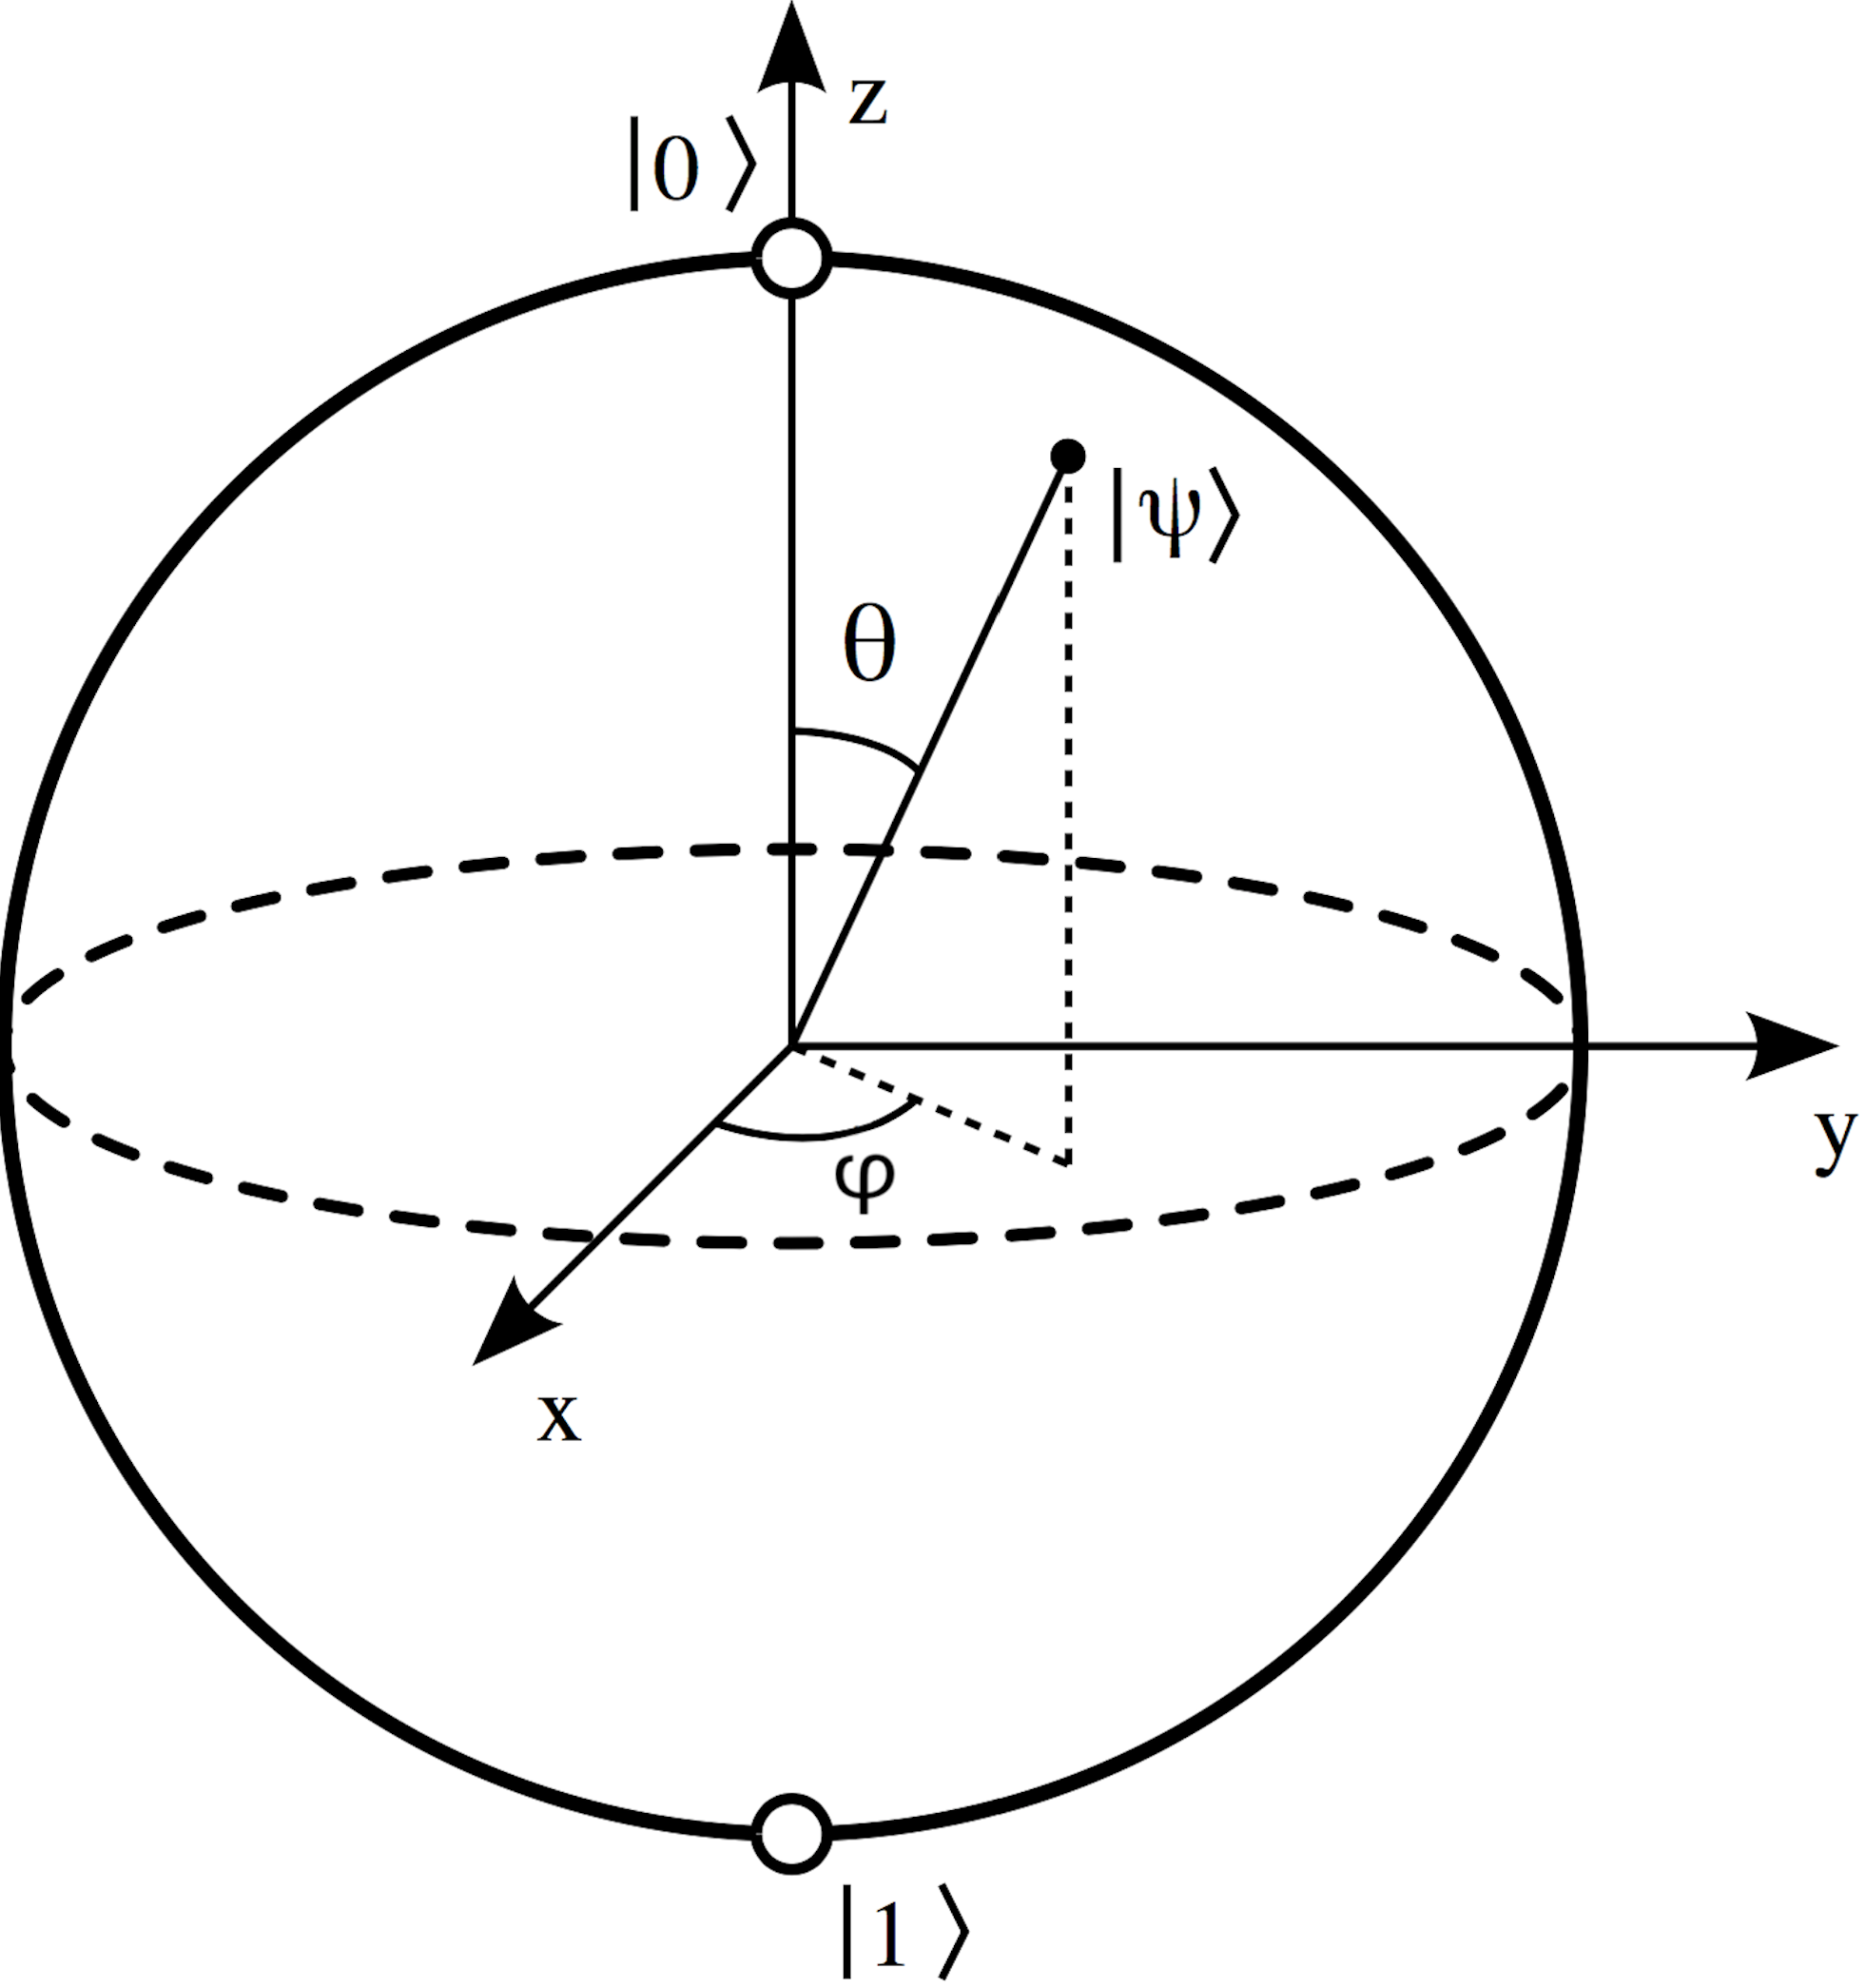
\includegraphics[width=2.0in]{images/blochSphere.png}
\caption{The Bloch sphere.}
\label{blochSphere}
\end{center}
\end{figure}

Many of the operations on a single qubit can be described within this sphere, which helps to grasp its intuitive meaning.

\paragraph{} There is a one-to-one correspondence between a generic state of a qubit
\begin{equation}
|\psi\rangle = \alpha|0\rangle + \beta|1\rangle
\label{eq:qubitStateDirac}
\end{equation}

and a point on the unit sphere in ${\mathbb{R}}^3$ represented as
\begin{equation}
cos\left(\frac{\theta}{2}\right)|0\rangle + e^{i\varphi}sin\left(\frac{\theta}{2}\right)|1\rangle
\label{eq:qubitStateBlock}
\end{equation}

where $\theta$ and $\varphi$ are real numbers (spherical coordinates of the point). To see this correspondence, it is necessary to know that there is another representation of complex numbers.

\subsubsection{Two equivalent representations}

\paragraph{} Look at the \autoref{complexPlane}: there is a graphical representation of the complex plane ${\mathbb{C}}$: it can be seen as a Cartesian plane with the \textit{real} axis on abscissas and the \textit{imaginary} axis part in ordinates.
\from{Matteo}{Create again the \autoref{complexPlane}}
\begin{figure}[!htb]
\begin{center}
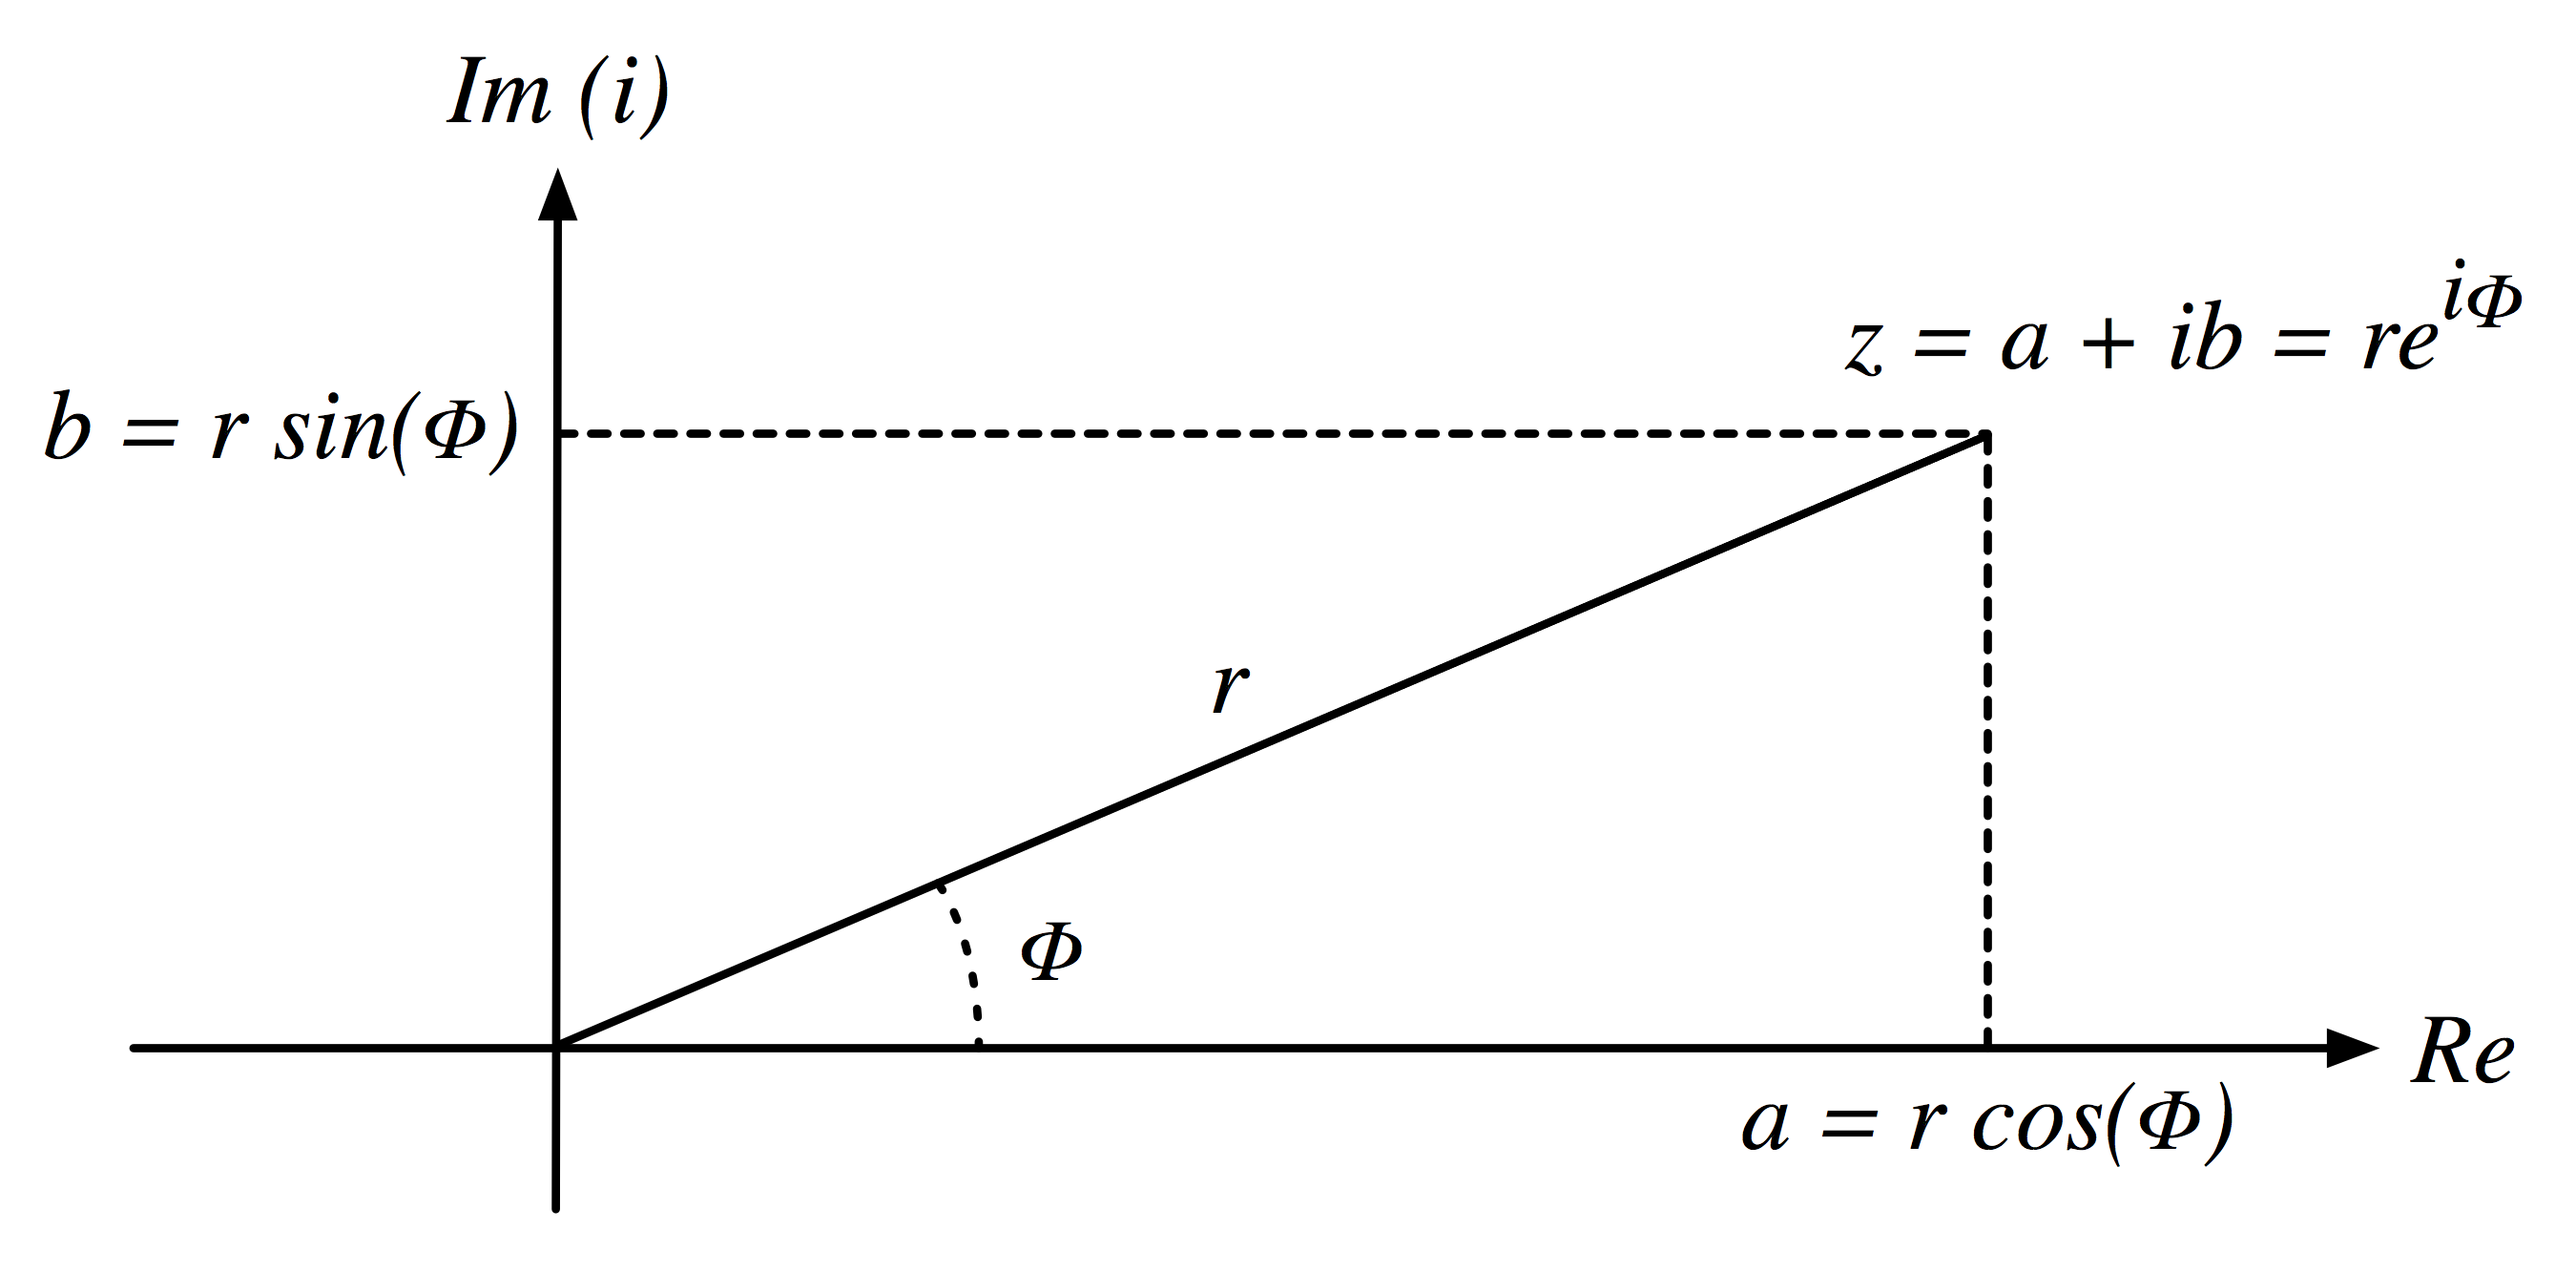
\includegraphics[width=3.3in]{images/complexPlane.png}
\caption{The complex plane.}
\label{complexPlane}
\end{center}
\end{figure}
\paragraph{Cartesian coordinates} Given a complex number $z \in \mathbb{C}$, $z$ is the point of coordinates $a$ on the real axis $Re$ and $b$ on the imaginary axis $Im$, i.e. $z = a + ib$, with $a, b \in \mathbb{R}$.

\paragraph{Polar coordinates} Let be $\phi$ the angle that the vector $z$ forms with the axis $Re$ and 
$$r = \sqrt{a^2 + b^2}$$
the norm of $z$, with 
$$a = rcos(\phi) \; \; \; \; \; b = rsin(\phi)$$
Thus, $z$ is identified by the coordinates $(r, \phi)$, i.e. 
$$z = a + ib = rcos(\phi) + risin(\phi)) = r(cos(\phi) + isin(\phi))$$

\begin{figure}[!htb]
\begin{center}
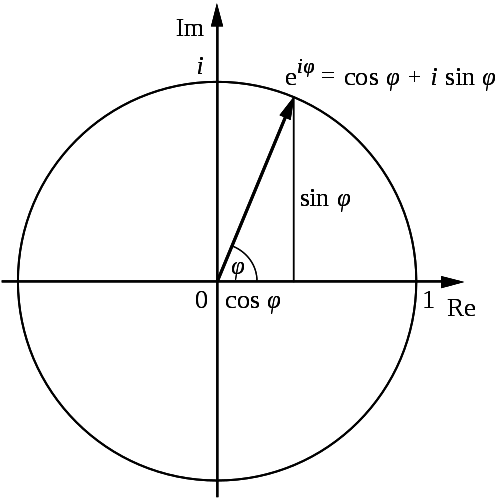
\includegraphics[width=2.2in]{images/euleroFormula.png}
\caption{Euler's formula graphical representation.}
\label{euleroFormula}
\end{center}
\end{figure}

Further, as shown in \autoref{euleroFormula}, Euler's formula states that for any real number $x$, it is always true that
\begin{equation}
e^{ix} = cos(x) + isin(x)
\label{eq:euleroFormula}
\end{equation}

with $e$ the base of the natural logarithm, $i$ the imaginary unit, and $cos$ and $sin$ the trigonometric functions cosine and sine respectively, with the argument $x$ given in radians. Thus, the complex number $z = r(cos(\phi) + isin(\phi))$ could be expressed as
\begin{equation}
z = r e^{i\phi}
\label{eq:complexNumberPolar}
\end{equation}

\paragraph{Qubit in geometry} A \textbf{qubit} is a two dimensional complex unitary\footnote{Unitary means that $\alpha$ and $\beta$ are complex numbers such that $|\alpha|^2 + |\beta|^2 = 1$.} vector $|\psi\rangle = \alpha|0\rangle + \beta|1\rangle$. Let be $\alpha = (r_0, \theta_0)$ and $\beta = (r_1, \theta_1)$, i.e. defined by using the respective polar coordinates. Thus $|\psi\rangle$ can be written as
\begin{equation}
|\psi\rangle = r_0 e^{i\theta_0}|0\rangle + r_1 e^{i\theta_1}|1\rangle \; \; \; \; \; \; with \; \; \; \; \; r_0^2 + r_1^2 = 1
\label{eq:qubitPolarStep}
\end{equation}

The condition over the the sum of the two complex numbers that compose vector state - $r_0^2 + r_1^2 = 1$ - is the equation that describes the points of the unit circle in ${\mathbb{R}}^2$, as shown in \autoref{circle}.

\begin{figure}[!htb]
\begin{center}
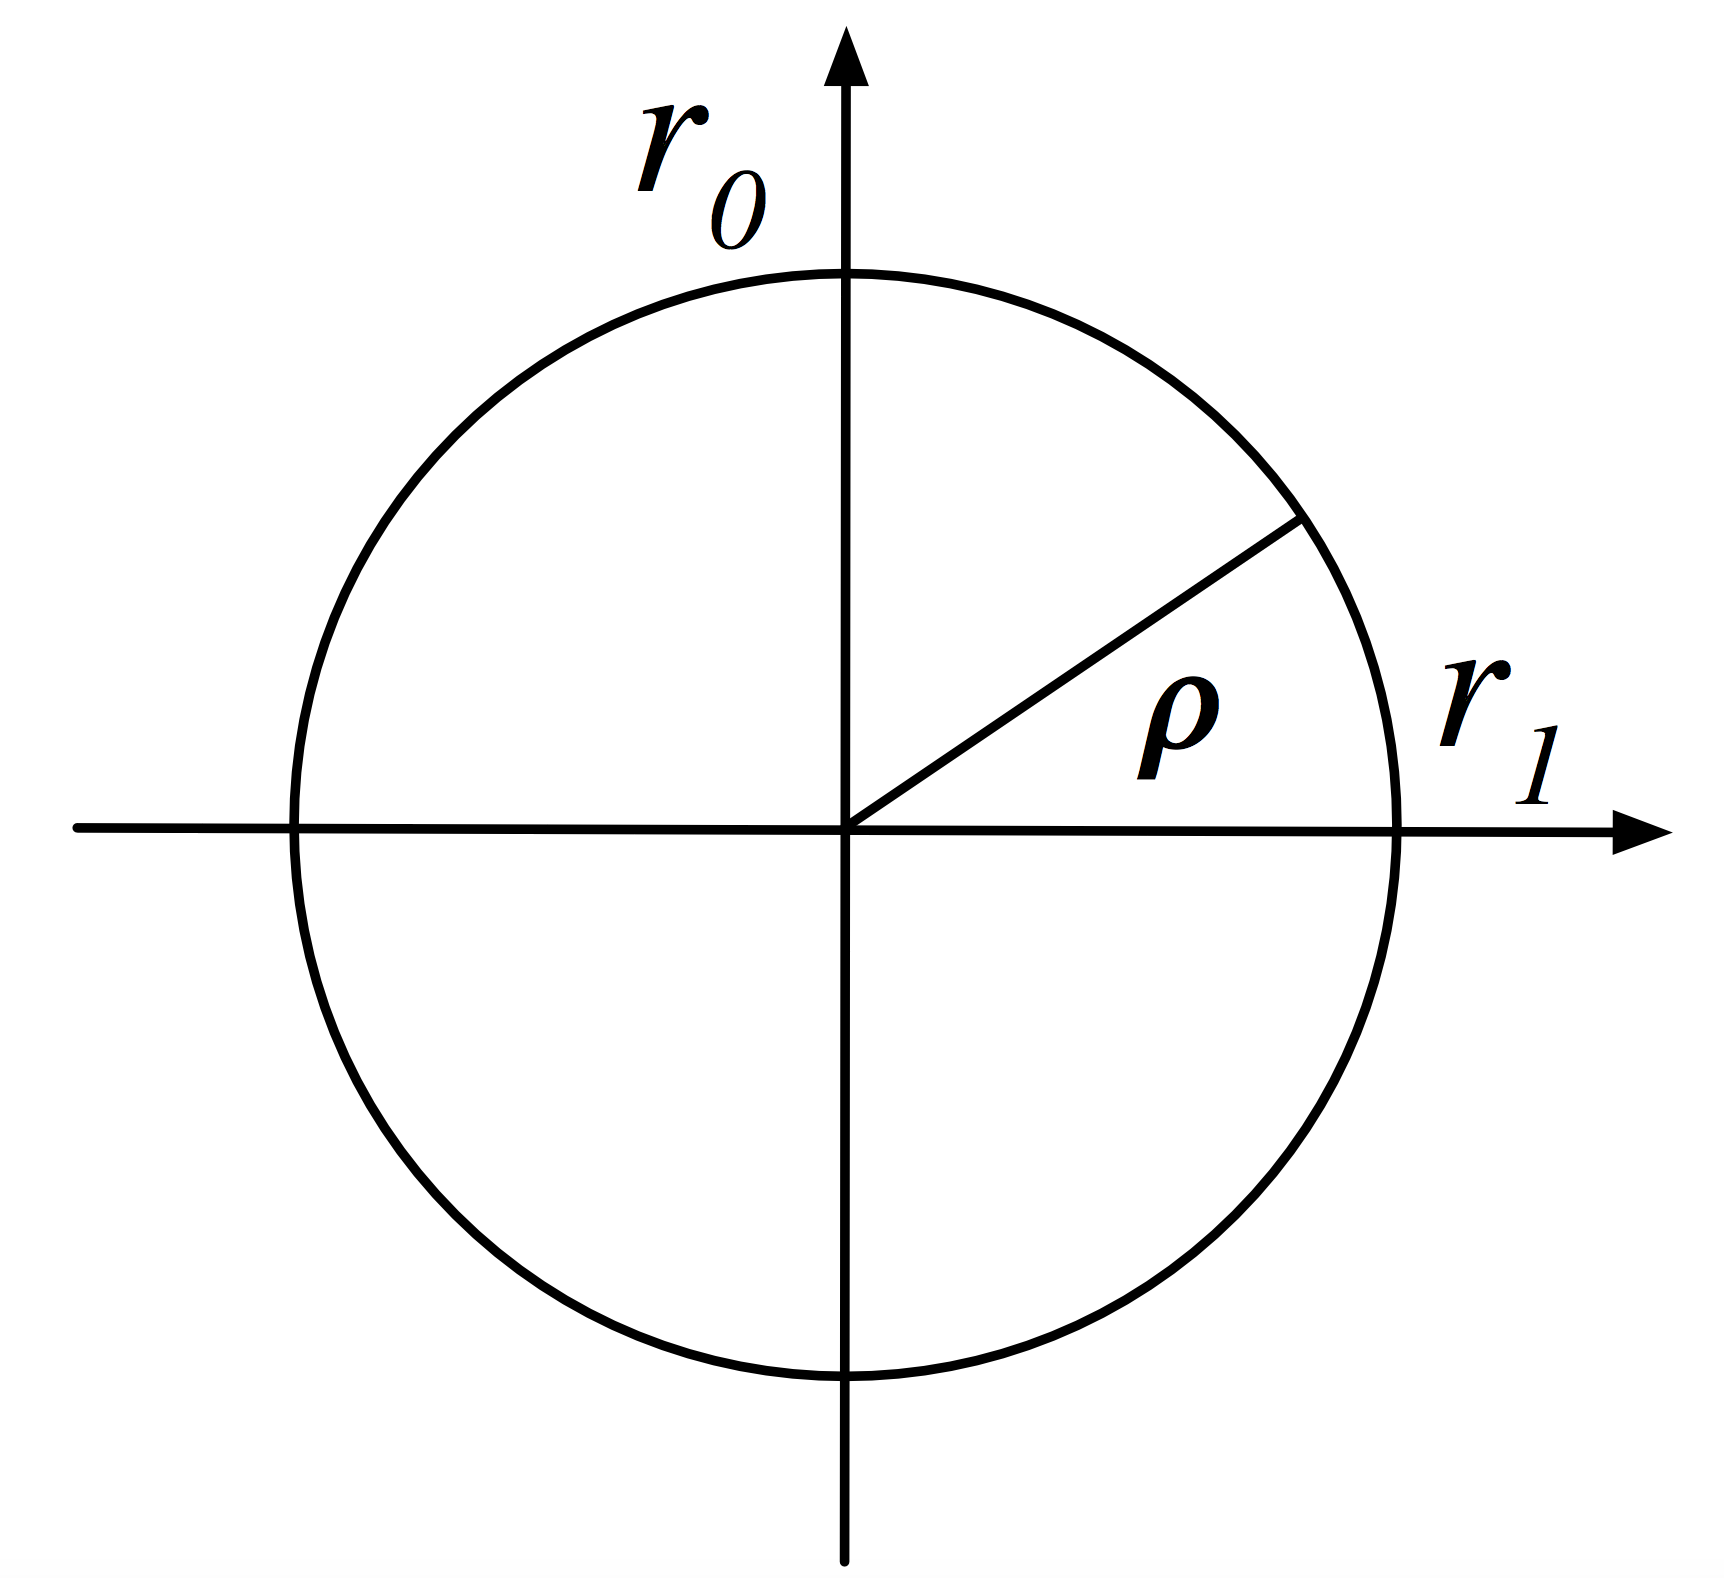
\includegraphics[width=1.8in]{images/circle.png}
\caption{The unit circle}
\label{circle}
\end{center}
\end{figure}

Thus, the modules of $\alpha$ and $\beta$ can be represented by using the angle $\rho$, placing
$$r_0 = cos(\rho) \; \; r_1 = sin(\rho)$$
By setting $\rho = \theta/2$ (one the two angle in the Block Sphere), we obtain the expression
$$|\psi\rangle = cos\left(\frac{\theta}{2}\right) e^{i\phi_0}|0\rangle + sin\left(\frac{\theta}{2}\right) e^{i\phi_1}|1\rangle$$
with $$0 \leq \theta \leq \pi$$
or, equivalently
$$|\psi\rangle = e^{i\gamma}\left(cos\left(\frac{\theta}{2}\right)|0\rangle + e^{i\varphi}sin\left(\frac{\theta}{2}\right)|1\rangle\right)$$
with $\varphi = \phi_1 - \phi_0$, $\gamma = \phi_0$ and $0 \leq \varphi \leq 2\pi$. 

\paragraph{} That's all. From a \textit{physical} point of view the factor $e^{i\gamma}$ (called \textit{global phase}) can be ignored because it has no observable effects, i.e. from the \textit{observational} point of view the two states $e^{i\gamma}|\psi\rangle$ and $|\psi\rangle$ are identical (from the principle of quantum measurement).
Finally, the spherical angle $\theta$ that a point on the unit sphere in ${\mathbb{R}}^3$ forms with the $z$ axis satisfies exactly the same condition $0 \leq \theta \leq \pi$ of the angle with $\theta$ in the representation of the qubit as cos $cos\left(\theta/2\right)|0\rangle + sin\left(\theta/2\right) e^{i\varphi}|1\rangle$. Also the angle $\varphi$ in this representation varies in the same interval $0 \leq \varphi \leq 2\pi$ of the angle that the projection of a unit vector in the Bloch sphere on the plane $(x, y)$ forms with the $x$ axis.

So there is actually a biunivocal correspondence between the qubits represented as:
$$cos\left(\theta/2\right)|0\rangle + sin\left(\theta/2\right) e^{i\varphi}|1\rangle$$
and the points on the Bloch sphere.

\paragraph{} Since we can code strings of arbitrary length in the number $\theta$, the classical information that a qubit can contain would seem infinite. However, the only way to extract the information contained in a qubit is through a measurement. According to the laws of quantum mechanics the result of this measurement is always a single classic bit - $0$ or $1$ - with probability that depends on the ``latitude" of the qubit.

\subsection{Physical interpretation}
\from{Matteo}{Improve this part}

\paragraph{} The abstract description of a qubit as a vector in a complex two-dimensional space has a correspondent in the real world. In particular, any physical system with at least two discrete and sufficiently separated energy levels is an appropriate candidate to represent a qubit. To physically create a qubit the three most common approaches are those based on:

\begin{itemize}
    \item the two different polarizations of a photon;
    \item the alignment of a nuclear spin in a uniform magnetic field;
    \item two levels of energy of an electron that orbits in a single atom;
\end{itemize}

For example, we can consider the system consisting of the $H^2$ hydrogen atom. In this system, the state $|0\rangle$ of the qubit can be represented by the first energy level ($n = 0$), corresponding to the base state of the electron, and the state $|1\rangle$ from the second energy level ($n = 1$) corresponding in the excited state of the electron. The passage of the electron from one state to another can be accomplished by subjecting the electron to a laser pulse of appropriate intensity, duration and wavelength. By appropriately reducing the duration, the passage of an electron can initially be carried out in the $|0\rangle$ state to a state that is "in the middle`` - between $|0\rangle$ and $|1\rangle$ - corresponding to the state $$\frac{1}{\sqrt{2}}|0\rangle + \frac{1}{\sqrt{2}}|1\rangle$$

When we look at a qubit, the result can only be $0$ or $1$. Furthermore, the measurement we have made changes the qubit's state by collapsing it from its overlap of $|0\rangle$ and $|1\rangle$ to the specific state consisting of the result of the measurement. These properties are explained by the principles of quantum mechanics.

\subsection{IBM Q} 

\subsubsection{Introduction}

\paragraph{} The IBM Quantum Experience is a tool provided by IBM to introduce the quantum world through a set of short tutorials and by providing the hands-on opportunity to experiment with operations on a real quantum computing processor. 

More formally, the IBM Quantum Experience is a cloud-based platform where you can learn, research, and interact with a real quantum computer housed in an IBM Research lab. The most important tools provided by the IBM team are:
\begin{enumerate}
    \item The \textbf{quantum composer} is a graphical interface tool where you can drag and drop different operations to control qubits. The quantum composer permits you to develop your own quantum algorithms, which IBM calls quantum scores.
    \item The \textbf{quantum score} is the set of instructions, or algorithm, to a quantum computer. It is a series of gates versus time played on different qubits, much like a musical score.
    \item The \textbf{quantum sphere} is the block sphere graphical representation of the output of a Quantum Score: IBM Q provides us a really cool way to easily visualize properties of the measurements performed on a number of qubits, all in one diagram.
\end{enumerate}

You can find more on these tools later in this guide.

\paragraph{} From a physical point of view, the qubit used by IBM is a fixed-frequency superconducting transmon qubit. It is a Josephson-junction-based qubit that is insensitive to charge noise. For more information on this type of qubit please see \cite{PhysRevA.76.042319}. They use fixed-frequency qubits, as opposed to tunable qubits, to minimize our sensitivity to external magnetic field fluctuations that could corrupt the quantum information.

The superconducting qubits are fabricated at IBM. The devices are made on silicon wafers with superconducting metals such as niobium and aluminum. Details about the fabrication processes are given in the site of IBM. The properties of the qubits can be seen below the quantum composer. Properties such as relaxation time (T1), coherence time (T2), readout errors, and gate errors are given, posted from the last calibration experiment run on the actual quantum processor device. 
The measurements of a qubit must be done in a way that does not destroy the qubit quantum state. One method is to weakly couple each qubit to a microwave resonator whose resonance characteristics depend on the state of the qubit. Once the qubit operations are completed in your score, you can measure the qubits by sending a microwave tone to their resonators and analyzing the signal it reflects back. The phase and amplitude of this reflected signal will be different depending on the qubit state. These signals in the resonator are boosted via a chain of amplifiers inside of our dilution refrigerator, including a quantum-limited amplifier at 15 mK, and a high-electron mobility transistor amplifier at 4 K.

Because the measurement of a qubit in a superposition state seems random – the outcome is sometimes 0 and sometimes 1 – you must repeat the measurement multiple times to determine the likelihood of a qubit being in a particular state. When performing the experiment, you will be asked how many \textit{shots} or experiments to run in order to determine the qubit state probabilities.

\subsubsection{IBM Rules}

\paragraph{} To make sure everyone has a chance to use the real device in IBM lab via the Cloud, IBM has established a \textbf{units currency system}. If you join the IBM Quantum Experience as a standard user, you have full access to their simulation capabilities and to previously-run cached results from the real device and a small number of units to run real experiments on the quantum processor hardware. Once you go ahead with experiments, you will be rewarded with extra units to run more real-time experiments. This system allows IBM experiment queue to run smoothly. When your units are used up, you will be replenished once you have viewed the results of the completed execution. IBM also invites standard users to request an upgrade of their user status to expert user, which provides access to more units and other advanced features as soon as they are introduced.
One last thing: the quantum processor in IBM lab requires frequent calibration; during these short periods, you will receive a ``down for calibration" notice and if we need to perform maintenance a ``down for maintenance" message will be displayed. In both cases the simulation will be available for you to keep learning and designing new experiments.

\newpage

\section{Quantum registers}

\paragraph{} With two classic bits we can form four possible states:
$$00, 01, 10, 11$$

In general, with $n$ bits it is possible to construct $2^n$ distinct states. The question is: how many states can be obtained with $n$ qubits? The space of the states generated by a system of $n$ qubits has $2^n$ dimensions: every vector normalized in this space represents a possible computational state\footnote{These are the \textbf{superpositions} introduced in \autoref{qubitvsbit}.}, which we will call quantum register of $n$ qubits. This exponential growth in the number of qubits of the size of the states space suggests the potential ability of a quantum computer to process information at a speed exponentially higher than that of a classical computer. Note that for $n = 200$ we get a number of dimensions that is larger than the number of atoms in the universe. 

\subsection{Definition}

\paragraph{} Formally a quantum register of $n$ qubit is an element of the $2^n$-dimensional Hilbert space, ${\mathbb{C}}^{2^n}$, with a computational base formed by $2^n$ registers each one composed by $n$ qubits:
$$|i_1\rangle\otimes|i_2\rangle\otimes\ldots|i_n\rangle$$
with $i_j \in \{0, 1\}, 1 \leq j \leq n$. For convenience, this base vector is written $|i_1\rangle|i_2\rangle\ldots|i_n\rangle$ or simply $|i_1 i_2\ldots i_n\rangle$. What does it means the $\otimes$ symbol?

\from{Matteo}{Move this part to the recall part}

In linear algebra, an \textbf{outer product} is the tensor product\footnote{More on this in the next pages.} of two coordinate vectors, a special case of the \textbf{Kronecker product} of matrices. The outer product of two coordinate vectors $\mathbf{u} \otimes \mathbf{v}$ is a matrix $\mathbf{w}$ such that the coordinates satisfy $w_{ij} = u_{i} v_{j}$.

\begin{equation*}
\begin{aligned}
\mathbf{u} \otimes \mathbf{v} = \mathbf{u} \mathbf{v}^{\mathrm{T}} = {\begin{bmatrix}
u_{1} \\
u_{2} \\
u_{3} \\
u_{4}
\end{bmatrix}}
{\begin{bmatrix}
v_{1} & v_{2} & v_{3}
\end{bmatrix}} = 
{\begin{bmatrix}
u_{1} v_{1} & u_{1} v_{2} & u_{1} v_{3} \\
u_{2} v_{1} & u_{2} v_{2} & u_{2} v_{3} \\ 
u_{3} v_{1} & u_{3} v_{2} & u_{3} v_{3} \\ 
u_{4} v_{1} & u_{4} v_{2} & u_{4} v_{3}
\end{bmatrix}}
\end{aligned}
\end{equation*}

\paragraph{Example} Consider the case of two qubits. In analogy with the single qubit, we can construct the computational base of the states space as the set of vectors $|00\rangle, |01\rangle, |10\rangle, |11\rangle$. As noted before, $|x, y\rangle$ is an abbreviation of $|x\rangle \otimes |y\rangle$, the tensor product of $x$ and $y$. In algebraic notation these vectors therefore correspond to

\begin{equation*}
\begin{aligned}
{\begin{bmatrix}
1 \\
0 \\
0 \\
0
\end{bmatrix}},
{\begin{bmatrix}
0 \\
1 \\
0 \\
0
\end{bmatrix}},
{\begin{bmatrix}
0 \\
0 \\
1 \\
0
\end{bmatrix}},
{\begin{bmatrix}
0 \\
0 \\
0 \\
1
\end{bmatrix}}
\end{aligned}
\end{equation*}

A quantum register of two qubits is an overlap state of the form:
$$|\psi\rangle = \alpha_{00}|00\rangle + \alpha_{01}|01\rangle + \alpha_{10}|10\rangle + \alpha_{11}|11\rangle$$

with $$\sum\limits_{i \in {\{0, 1\}}^2}{|\alpha_i|}^2 = 1$$

\paragraph{NOTE} The two qubits quantum register is represented with two-ket notation basis ($|00\rangle, |01\rangle, |10\rangle, |11\rangle$). This is because, of course, each possible state of the two qubits handled could be a linear combination of the four possible states they will collapse to when measured.

In a $n$ qubit system we can also measure only a subset of $n$ qubits. For instance, in the case of a two-qubit register we can measure the first qubit, resulting in $0$ with probability $|\alpha{00}|^2 +|\alpha{01}|^2 $. After measuring, the status will collapse to
$$\frac{\alpha_{00}|00\rangle + \alpha_{01}|01\rangle}{\sqrt{|\alpha_{00}|^2 + |\alpha_{01}|^2}}$$

\paragraph{Exercise} Look at exercise number 2 in \autoref{exs}.

\subsection{Entangled states}

\paragraph{} An important property of the quantum registers made of $n$ qubit is that it is not always possible to \texttt{decompose} them into the states of the qubits components. The states of this type are called \textbf{entangled} and have properties that can not be found in any other objects in classical physics. 

To quote IBM Q official site, the quantum computer takes advantage of this special kind of superposition that allows for \textit{exponentially many} logical states at once, all the states from $|00\ldots00\rangle$ to $|11\ldots11\rangle$.

Members of an entangled collection do not have their own individual status, but the entire collection they belong to has a well-defined state. The entangled states behave as if they were closely connected to each other, regardless of the distance that separates them. For example, a measurement of one of the two states of an entangled pair simultaneously provides information about the other. This property is a powerful feat, the basis for solutions to problems in information processing that can not be reproduced classically.

A working quantum computer could factor numbers in a day that would take a classical computer millions of years. An example shown below will be the realization of quantum circuits for the teleportation of a quantum state from one location to another.

\paragraph{Entanglement}
\label{entanglement}
The state $|00\rangle + |11\rangle$ can not be factored into the tensor product of two independent qubits, i.e. there is no $a_1, a_2, b_1, b_2$ such that $|00\rangle + |11\rangle = (a_1 |0\rangle + b_1 |1\rangle) \otimes (a_2 |0\rangle + b_2 |1\rangle$).

\paragraph{Exercise} Look at exercise 7 in \autoref{exs}.

\newpage

\section*{Introduction to quantum circuits}

\section{Quantum logical gates} 
\label{sec:section5}
\paragraph{} Until know the quantum description of the states of a computation has been introduced. Let's see now how these states evolve giving rise to a quantum computation. Like classical computers, a quantum computer is made up of quantum circuits made up of elementary quantum logic gates. In the classical case there is a single logical (non-trivial) one-bit port, the \texttt{NOT} gate, which implements the logical negation operation defined by a truth table in which $1 \rightarrow{} 0$ and $0 \rightarrow{} 1$.

To define a similar operation on a qubit, we can not limit ourselves to establishing its action on the base states $|0\rangle$ and $|1\rangle$, but we must also specify how a qubit must be transformed which is in an overlap of states $|0\rangle$ and $|1\rangle$. Intuitively, the \texttt{NOT} should exchange the roles of the two fundamental states and transform $\alpha|0\rangle + \beta|1\rangle$ into $\beta|0\rangle + \alpha|1\rangle$ - this is not to say that $\alpha$ becomes $beta$, but rather that $0\rangle$ would turn into $1\rangle$ and $1\rangle$ to $0\rangle$. The operation that implements this type of transformation is a linear operation (see math section on that \from{Matteo}{Todo: add ref to linear operator.}) and it is a general property of quantum mechanics experimentally justified. A convenient way to represent linear operations is by using matrices.

\subsection{One qubit quantum logic gates}

\paragraph{Pauli matrices} The following matrices are unitary:
\begin{equation}
\begin{aligned}
X = \begin{bmatrix}
0 & 1 \\
1 & 0 \\
\end{bmatrix} \; \; \; 
Y = \begin{bmatrix}
0 & i \\
-i & 0 \\
\end{bmatrix} \; \; \;
Z = \begin{bmatrix}
1 & 0 \\
0 & -1 \\
\end{bmatrix}
\end{aligned}
\label{eq:pauliMatrices}
\end{equation}
they are unitary. $X, Y, Z$ are called \textbf{Pauli matrices}.

\subsubsection{The \texttt{X} gate}

\paragraph{} The Pauli \texttt{X} gate is known as an $X_{\pi}$-rotation. It takes $|0\rangle \rightarrow{} X|0\rangle = |1\rangle$: in other words, it flips the zero to a one, or vice versa (this is why it is also commonly referred to as a bit-flip). It's corresponding to the quantum \texttt{NOT} and it is represented by the matrix
$$X = \begin{bmatrix}
0 & 1 \\
1 & 0 \\
\end{bmatrix}$$
Thus,
$$X|0\rangle = \begin{bmatrix}
0 & 1 \\
1 & 0 \\
\end{bmatrix} \begin{bmatrix}
1 \\
0 \\
\end{bmatrix} = \begin{bmatrix}
0+0 \\
1+0 \\
\end{bmatrix} = \begin{bmatrix}
0 \\
1 \\
\end{bmatrix}$$
And
$$X|1\rangle = \begin{bmatrix}
0 & 1 \\
1 & 0 \\
\end{bmatrix} \begin{bmatrix}
0 \\
1 \\
\end{bmatrix} = \begin{bmatrix}
0+1 \\
0+0 \\
\end{bmatrix} = \begin{bmatrix}
1 \\
0 \\
\end{bmatrix}$$

It is possible to verified that the application of \texttt{X} to a qubit $\alpha|0\rangle + \beta|1\rangle$ (written in vector notation) is
$$X\begin{bmatrix}
\alpha \\
\beta \\
\end{bmatrix} = \begin{bmatrix}
0 & 1 \\
1 & 0 \\
\end{bmatrix} \begin{bmatrix}
\alpha \\
\beta \\
\end{bmatrix}$$

\subsubsection{The \texttt{Y} gate}

\paragraph{} The Pauli \texttt{Y} gate acts on a single qubit. It equates to a rotation around the $Y$-axis of the Bloch sphere by $\pi$ radians. It is represented by the matrix
$$Y = \begin{bmatrix}
0 & -i \\
i & 0 \\
\end{bmatrix}$$
It maps
$$Y|0\rangle = \begin{bmatrix}
0 & -i \\
i & 0 \\
\end{bmatrix} \begin{bmatrix}
1 \\
0 \\
\end{bmatrix} = \begin{bmatrix}
0+0 \\
i+0 \\
\end{bmatrix} = \begin{bmatrix}
0 \\
i \\
\end{bmatrix} = i\begin{bmatrix}
0 \\
1 \\
\end{bmatrix} = i|1\rangle$$
And
It maps
$$Y|1\rangle = \begin{bmatrix}
0 & -i \\
i & 0 \\
\end{bmatrix} \begin{bmatrix}
0 \\
1 \\
\end{bmatrix} = \begin{bmatrix}
0-i \\
0+0 \\
\end{bmatrix} = \begin{bmatrix}
-i \\
0 \\
\end{bmatrix} = -i\begin{bmatrix}
1 \\
0 \\
\end{bmatrix} = -i|0\rangle$$

\subsubsection{The \texttt{Z} gate}

\paragraph{} The Pauli \texttt{Z} gate acts on a single qubit. It equates to a rotation around the \texttt{Z} axis of the Bloch sphere by 
$\pi$ radians: it is a special case of a phase shift gate (next) with $\phi = \pi$. It leaves the basis state $|0\rangle$ unchanged and maps $|1\rangle$ to $-|1\rangle$. Due to this nature, it is sometimes called phase-flip. It is represented by the matrix
$$Z = \begin{bmatrix}
1 & 0 \\
0 & -1 \\
\end{bmatrix}$$
It maps
$$Z|0\rangle = \begin{bmatrix}
1 & 0 \\
0 & -1 \\
\end{bmatrix} \begin{bmatrix}
1 \\
0 \\
\end{bmatrix} = \begin{bmatrix}
1+0 \\
0+0 \\
\end{bmatrix} = \begin{bmatrix}
1 \\
0 \\
\end{bmatrix} = |0\rangle$$
And
$$Z|1\rangle = \begin{bmatrix}
1 & 0 \\
0 & -1 \\
\end{bmatrix} \begin{bmatrix}
0 \\
1 \\
\end{bmatrix} = \begin{bmatrix}
0+0 \\
0-1 \\
\end{bmatrix} = -\begin{bmatrix}
0 \\
1 \\
\end{bmatrix} = -|1\rangle$$

\paragraph{Property} Note that $I^2 = X^2 = Y^2 = Z^2 = I$.

\paragraph{Exercise} Look at exercises 13, 14 and 15 in \autoref{exs}.

The Pauli matrices represents respectively the components $x$, $z$, $y$ of the spin of an electron. It can be shown that for each unitary matrix $U$ (see \from{Matteo}{RECALL}) there are real numbers $\alpha, \beta, \delta, \gamma$ such that:

\begin{equation}
\begin{aligned}
U = \begin{bmatrix}
e^{i(\alpha - \frac{\beta}{2} - \frac{\delta}{2})}cos(\frac{\gamma}{2}) & -e^{i(\alpha - \frac{\beta}{2} + \frac{\delta}{2})}sin(\frac{\gamma}{2}) \\
e^{i(\alpha + \frac{\beta}{2} - \frac{\delta}{2})}sin(\frac{\gamma}{2}) & e^{i(\alpha + \frac{\beta}{2} + \frac{\delta}{2})}cos(\frac{\gamma}{2})
\end{bmatrix}
\end{aligned}
\label{eq:unitaryMatrixTheorem}
\end{equation}

\paragraph{Exercise} Look at exercise 16 in \autoref{exs}.

\subsubsection{The \texttt{Hadamard}, \texttt{S} and \texttt{T} gate}

\from{Matteo}{Review this part and transformation...something is wrong}

\paragraph{} There are some other important gates to talk about, such as \texttt{S}, \texttt{T} and \texttt{H}. The latter is called the Hadamard gate and it is one of the most important gate in quantum world. The matrices of this three gates are shown below.
\begin{equation}
\begin{aligned}
S = \begin{bmatrix}
1 & 0 \\
0 & i \\
\end{bmatrix} \; \; \; \\
{\displaystyle {T} = {\sqrt {S}}={\sqrt {\mbox{SWAP}}}={\begin{bmatrix}1&0&0&0\\0&{\frac {1}{2}}(1+i)&{\frac {1}{2}}(1-i)&0\\0&{\frac {1}{2}}(1-i)&{\frac {1}{2}}(1+i)&0\\0&0&0&1\\\end{bmatrix}}} \; \; \; \\
H = \frac{1}{\sqrt{2}}\begin{bmatrix}
1 & 1 \\
1 & -1 \\
\end{bmatrix}
\end{aligned}
\label{eq:sthGates}
\end{equation}

[1,0],[0,(1+1i)/sqrt(2)]][[1,0],

There are also other two available gates in the \texttt{IBM Q} interface and specification: the $T^\dagger$ and $S^\dagger$. The respective transformation matrix are 
\begin{equation}
\begin{aligned}
S^\dagger = \begin{bmatrix}
1 & 0 \\
0 & -i \\
\end{bmatrix} \; \; \; \\
{\displaystyle {T^\dagger} = {\sqrt {\mbox{SWAP}}}={\begin{bmatrix}1&0&0&0\\0&{\frac {1}{2}}(1-i)&{\frac {1}{2}}(1+i)&0\\0&{\frac {1}{2}}(1+i)&{\frac {1}{2}}(1-i)&0\\0&0&0&1\\\end{bmatrix}}} \; \; \; \\
\end{aligned}
\label{eq:sttdGates}
\end{equation}

\subsection{IBM quantum composer}

\paragraph{} The quantum composer is the official IBM graphical user interface for programming a quantum processor. The composer is a tool to construct quantum circuits using a library of well-defined gates and measurements. You can create your own account in IBM using Github sign up starting from \href{https://quantumexperience.ng.bluemix.net/}{quantum experience} site.

When you first click on the ``Composer" tab above, you will have a choice between running a real quantum processor or a custom quantum processor. In the custom processor, gates can be placed anywhere, whereas in the real processor, the topology is set by the physical device running in our lab (note that this restricts the usability of some of the two-qubit gates).
Once you are in the ``Composer" tab, you can start making your very own quantum circuits. The IBM quantum composer is shown in \autoref{ibmComposer}.

\begin{figure}[!htb]
\begin{center}
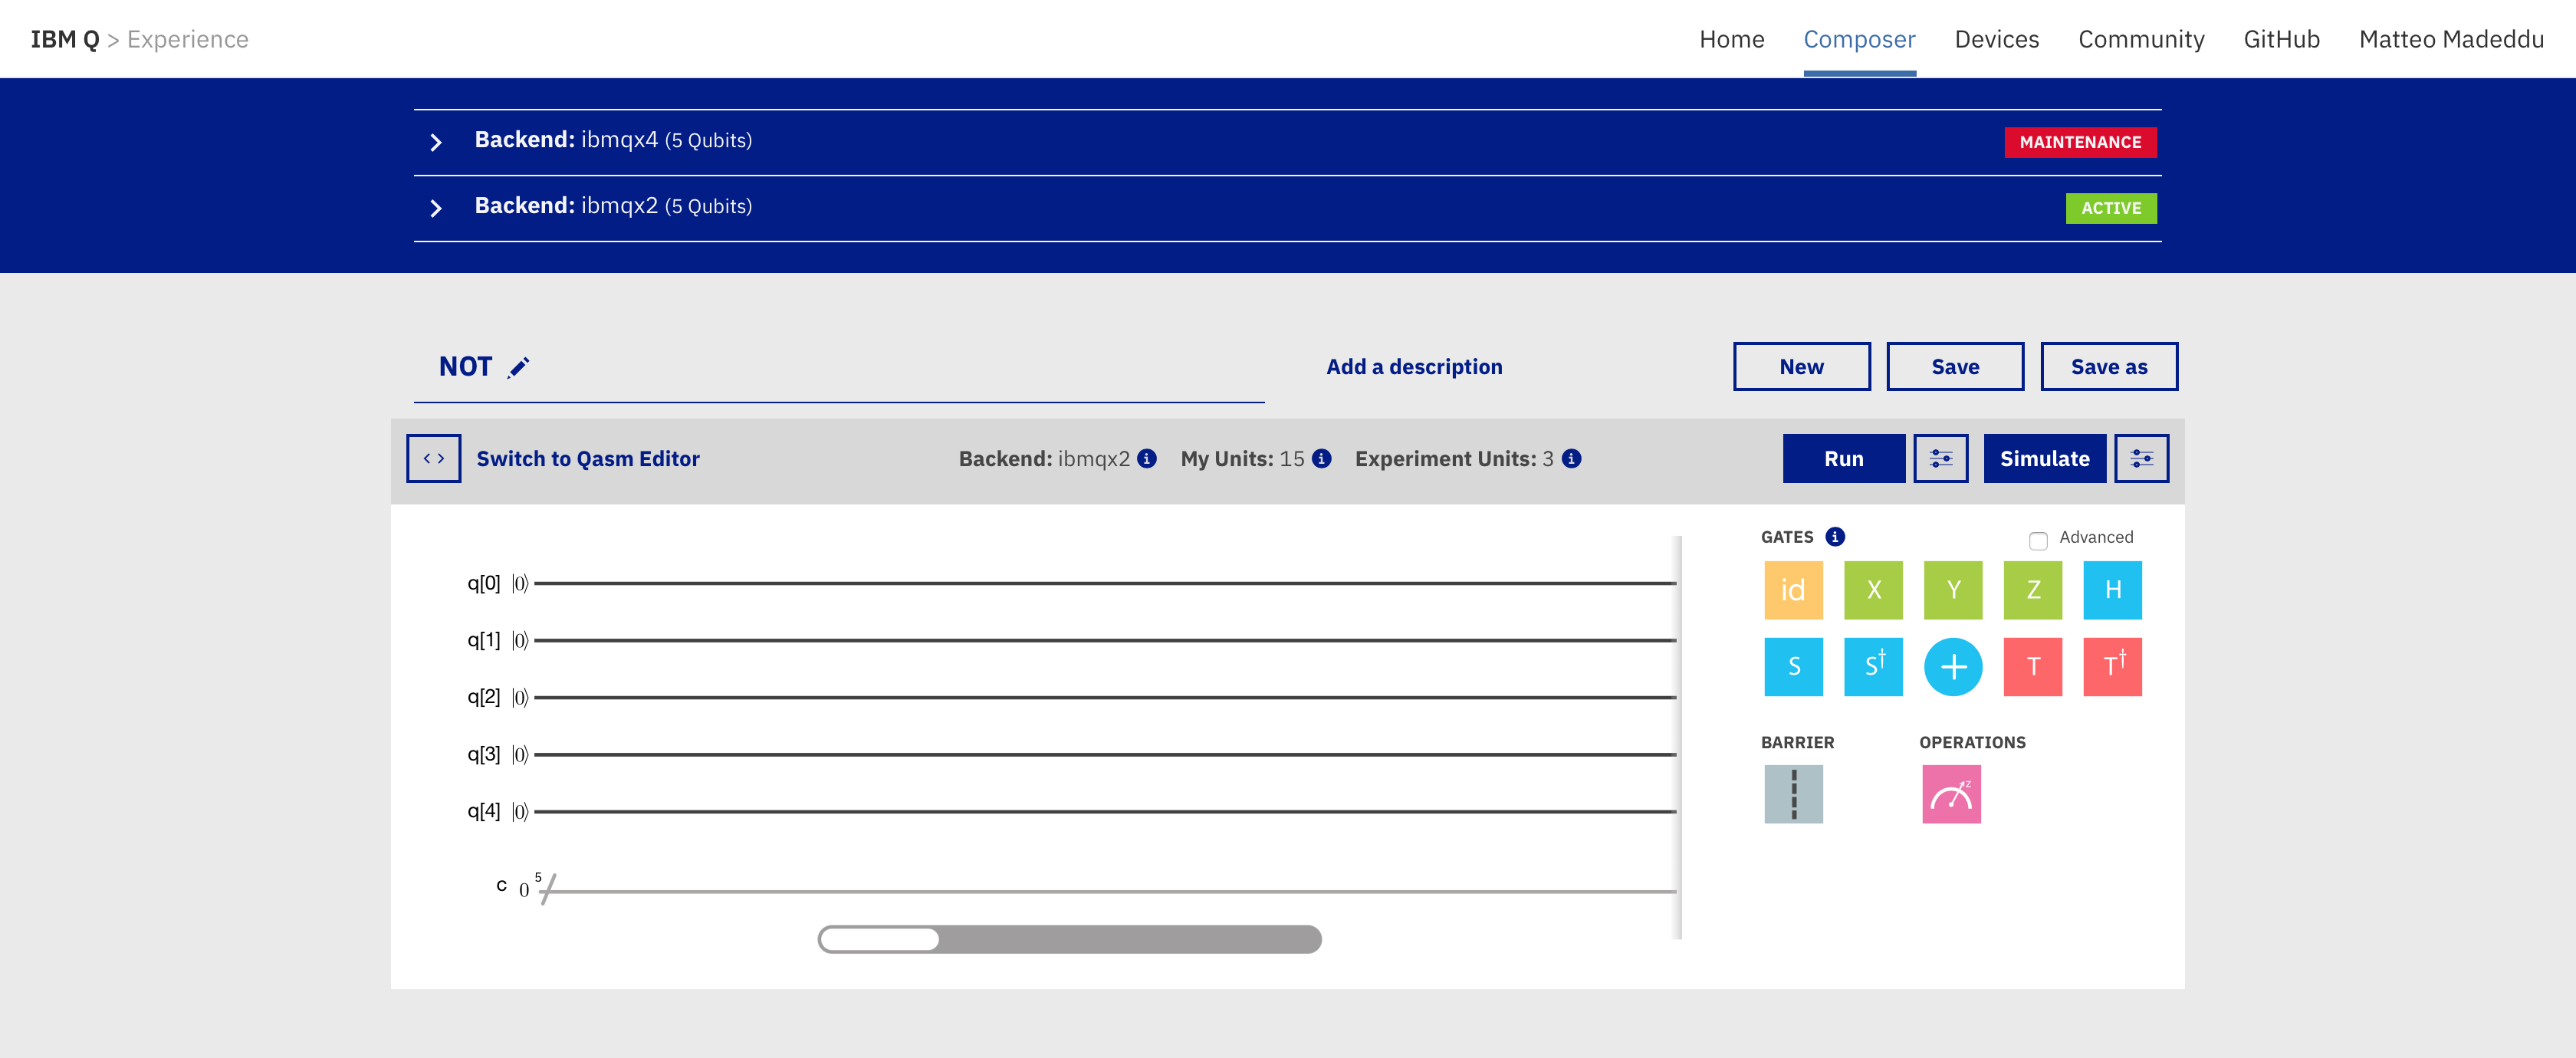
\includegraphics[width=4.7in]{images/ibmComposer.png}
\caption{The IBM quantum composer available at \href{https://quantumexperience.ng.bluemix.net/}{quantum experience}.}
\label{ibmComposer}
\end{center}
\end{figure}

With the composer, you can create a quantum score, which is analogous to a musical score in several respects. Time progresses from left to right. Each line represents a qubit (as well as what happens to that qubit over time). Each qubit has a different frequency, like a different musical note. The quantum composer's library (located to the right of the qubit stave) contains many different classes of gates: single-qubit gates, such as the yellow idle operation; the green class of \textbf{Pauli operators}, which represent bit-flips (X, equivalent to a classical NOT); phase-flips (Z); and a combined bit-flip and phase-flip (Y). There are others gates available that haven't been introduced yet. In general, quantum gates are represented by square boxes that play a frequency for different durations, amplitudes, and phases. Gates on just one line are called single-qubit gates. Before going on with esperiments, let's introduce these kind of gates.

\subsubsection{IBM Q - First Experiment} 

\paragraph{} When you begin an experiment, you'll be prompted to give it a name, so that you can recognize it later. You will also see two choices: real quantum processor, or custom topology.  In both cases, you create your score by dragging gates onto the stave, adding a measurement, and then hitting ``run" for the score to execute.

If you select ``Custom Topology" your only option is to run your score in simulation. This is because the custom processor permits all-to-all connectivity; the real device, in contrast, is limited by physical connectivity. When you select custom topology, a dialogue box will ask you to select the number of qubits and classical bits assigned to different registers. IBM have set the maximum number of qubits to 20.

The operation $M$ consists in the measurement of a qubit. If you measure, for instance, $|\psi\rangle = \alpha|0\rangle + \beta|0\rangle$, you know the result is a classic bit $M$ (indicated with a double line) that will be $0$ or $1$ with probability respectively ${|\alpha|}^2$ an ${|\beta|}^2$.

The execution of your circuit happens immediately (unless the number of qubits is large) and the output can then be viewed in the results. You can try the ``single qubit measurement" show in \autoref{ibmComposerSimpleEmulated}.

\begin{figure}[!htb]
\begin{center}
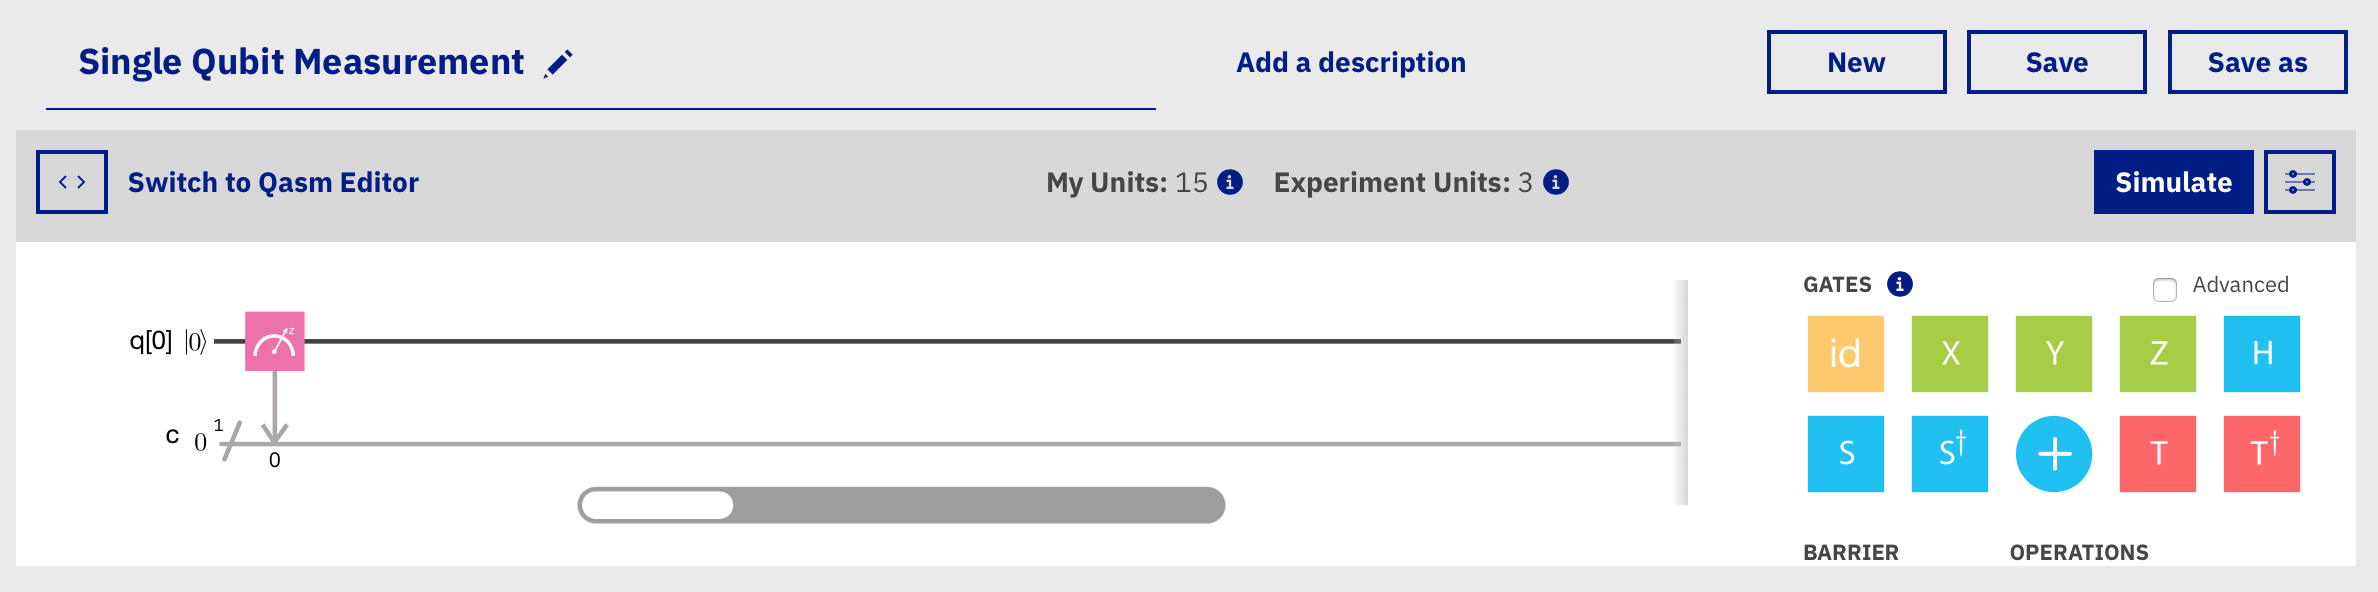
\includegraphics[width=4.7in]{images/ibmComposerSimpleEmulated.png}
\caption{The setup of a measurement in the IBM quantum composer over a single qubit in a \textbf{simulated} quantum processor.}
\label{ibmComposerSimpleEmulated}
\end{center}
\end{figure}

If you have chosen a real quantum processor, the composer will look like the one shown in \autoref{ibmComposerSimpleReal}.
\begin{figure}[!htb]
\begin{center}
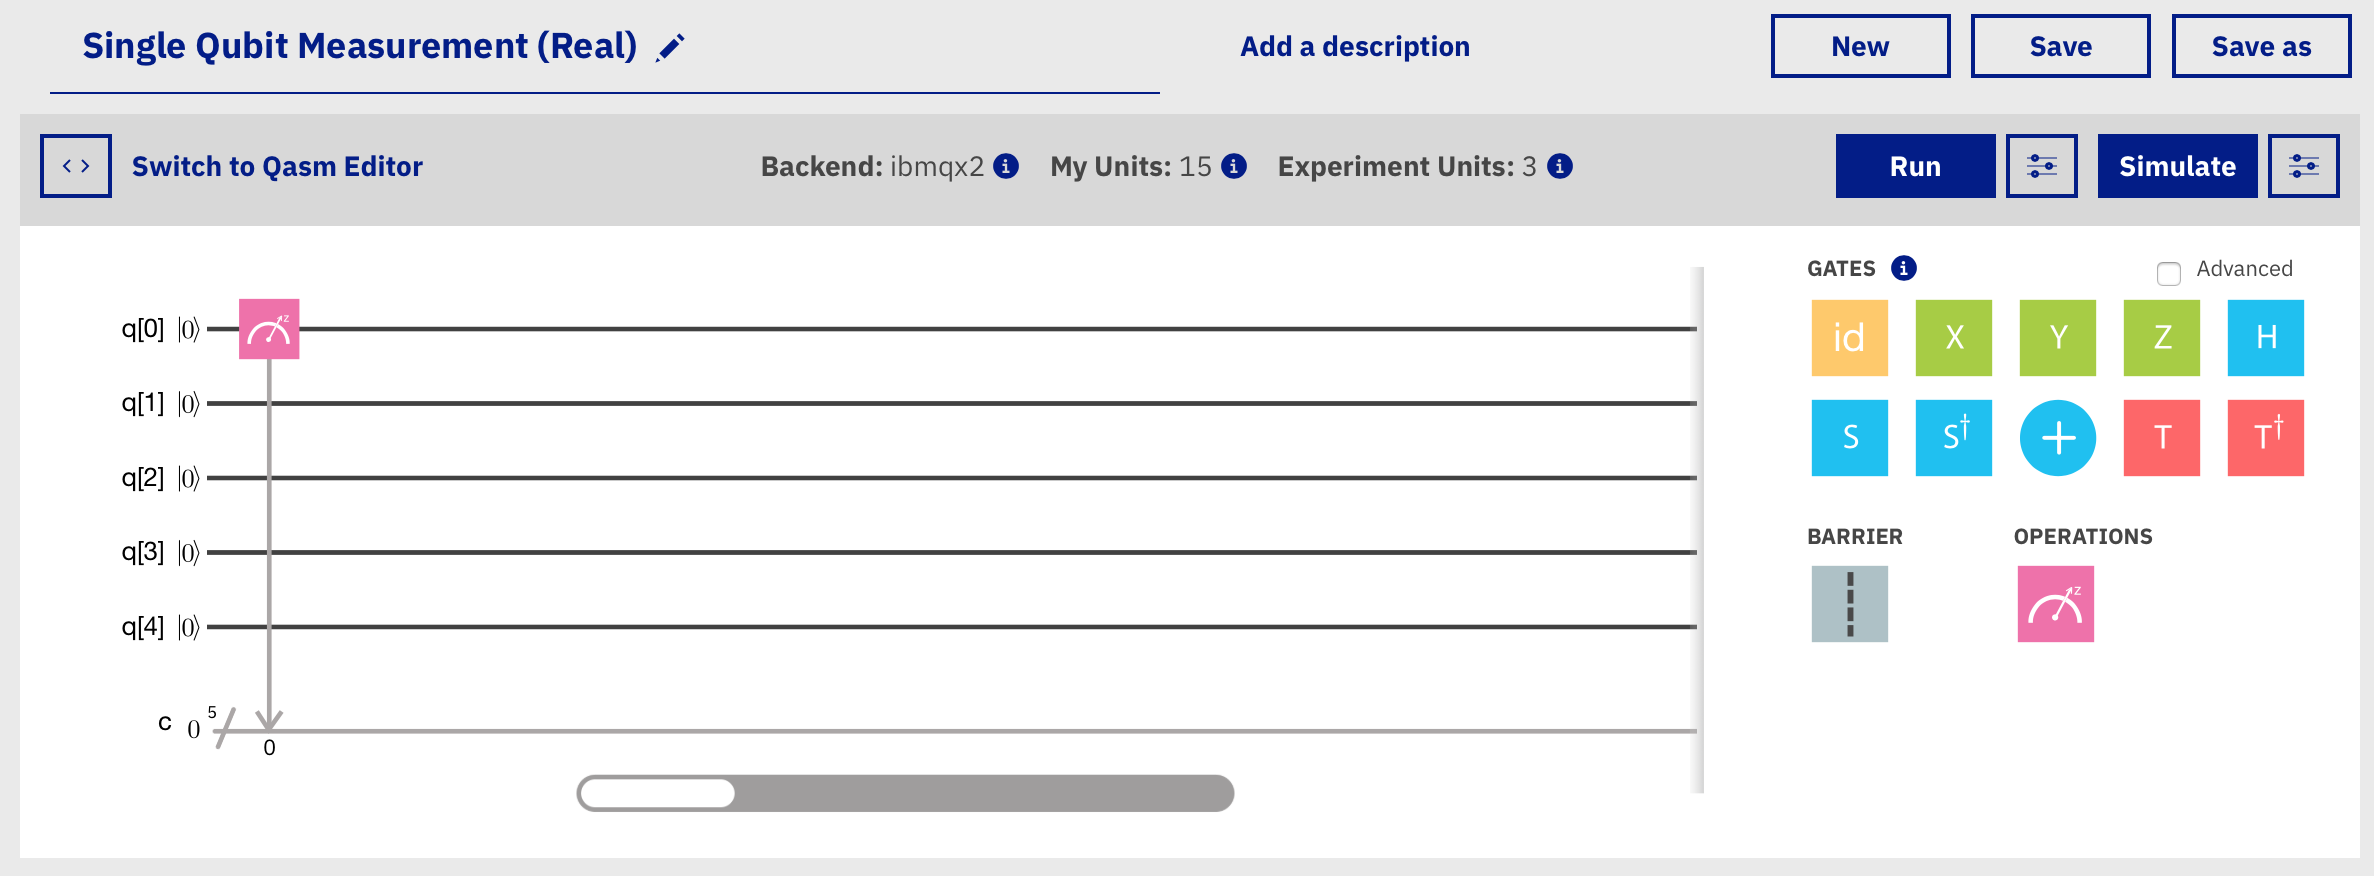
\includegraphics[width=4.7in]{images/ibmComposerSimpleReal.png}
\caption{The setup of a measurement in the IBM quantum composer over a single qubit in a \textbf{real} quantum processor.}
\label{ibmComposerSimpleReal}
\end{center}
\end{figure}

In IBM quantum experience, the results from launching your quantum scores can be visualized in two different ways: a standard histogram/bar graph, and as a quantum sphere, or QSphere - the Block Sphere introduced before. The QSphere represents quantum circuit measurement outcomes in a visually striking and information-dense graphic.

After performing a quantum measurement, a qubit's information becomes a classical bit, and in our system (as is standard) the measurements are performed in the computational basis. For each qubit the measurement either takes the value 0 if the qubit is measured in state $|0\rangle$ and value $|1\rangle$ if the qubit is measured in state $|1\rangle$.

In a given run of a quantum circuit with $n$ measurements, the result will be one of the $2^n$ possible $n$-bit binary strings. If the experiment is run a second time, even if the measurement is perfect and has no error, the outcome may be different due to the fundamental randomness of quantum physics. The results of a quantum circuit executed many different times can be represented as a distribution over the full $2^n$ possible outcomes. It is not scalable to represent all possible outcomes; therefore, we keep only those outcomes that happen in a given experiment and represent them in two different ways: as bars or as a quantum sphere.

\begin{enumerate}
    \item The \textbf{histogram representation} is the simplest to understand. The height of the bar represents the fraction of instances the outcome comes up in the different runs on the experiment. Only those outcomes that occurred with non-zero occurrences are included. If all the bars are small for visualization only (not if you download the data) they are collected into single bar called \textit{other values}. In general this is not a problem as a good quantum circuit should not have many outcomes only circuits that have the final state in a large superposition will give many outcomes and these would take exponential measurements to measure.
    \item The \textbf{quantum sphere representation} (QSphere) is the IBM tool to visually show the same data as the bar graph neatly and strikingly. Each line from the center represents a possible outcome of the experiment, and the weight (darkness of the line) represents the likelihood of each outcome. As with the histogram, only those outcomes are included that occurred in a given experiment. The QSphere is divided into $n+1$ levels, and each section represents the weight (total number of $1$s) of the binary outcome. The top is the $|0\ldots0\rangle$ outcome, the next line is all the outcomes with a single 1 ($|10\ldots0\rangle$, $|01\ldots0\rangle$, etc), the line after that is all outcomes with two $1$s, and so on until the bottom that is the outcome $|1\ldots1\rangle$. 
    
    For a single qubit there are two outcomes, and the sphere has only two levels; for two qubits, it has three sections with the middle section separated into two parts; for three qubits, it has four sections with the middle two being broken into three sections, and so on, following Pascal’s triangle shown in \autoref{ibmQuantumSphereLevelsOutcome}.
    
    \begin{figure}[!htb]
    \begin{center}
    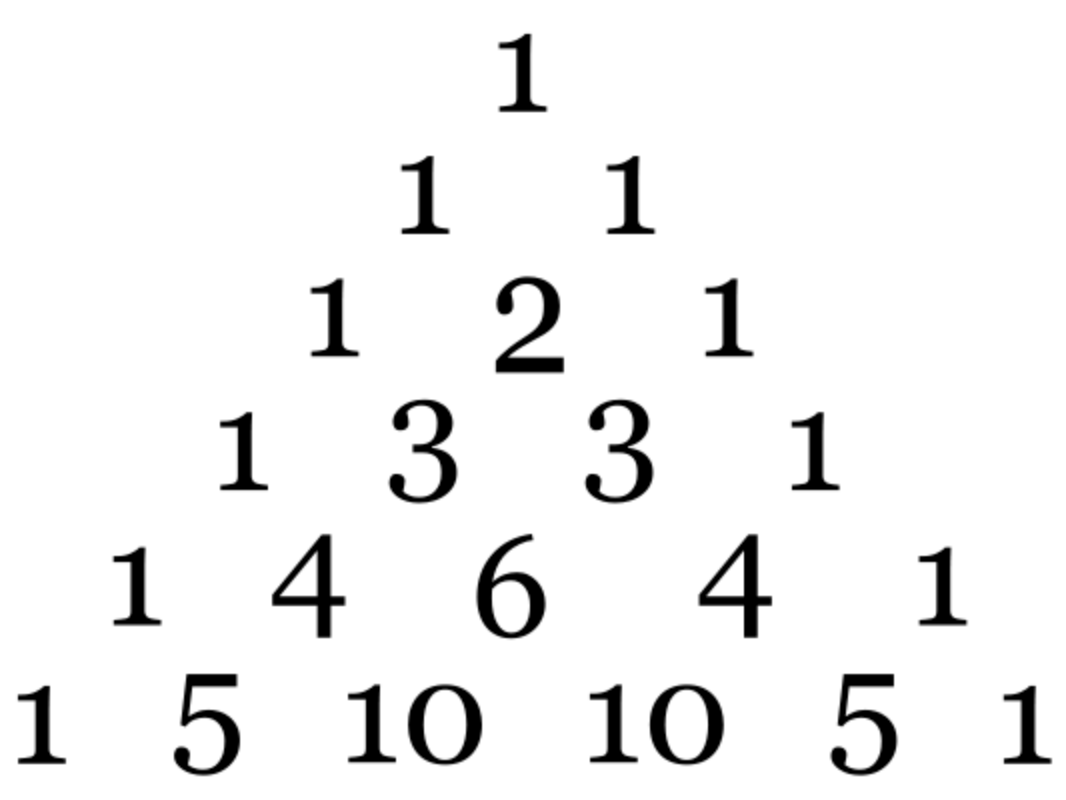
\includegraphics[width=2.5in]{images/ibmQuantumSphereLevelsOutcome.png}
    \caption{The IBM Quantum (Block) Sphere levels outcome separation follows the Pascal’s triangle.}
    \label{ibmQuantumSphereLevelsOutcome}
    \end{center}
    \end{figure}
    The usefulness of the Block Sphere representation is for distinguishing classical states from entangled states. A computational basis state will have a single line pointing in one direction. Under the assumption the state is pure, a superposition of two basis states will have two lines pointing in two directions of half weight. If these directions are on opposite sides of the QSphere we have a state that is maximally entangled (for $n>1$) in the computation bases. Finally if there are faint lines in every direction we have made a uniform superposition state.
\end{enumerate}

\subsubsection{IBM Q - Testing the gates} The configuration to test the effect of \texttt{X} gate is really simple: first, drag and drop an \texttt{X} gate on the first qubit (first line) - time is discrete, divided in several dots. The initial state of each qubit is $|0\rangle$.

In general, an operation on a single qubit can be specified by a $2 \times 2$ matrix. However, not all $2 \times 2$ arrays define ``legitimate" operations on qubits. We recall that the normalization condition requires that $\alpha^{2} + \beta^{2}$ in any quantum state $\alpha|0\rangle + \beta|1\rangle$. The same condition must also apply to the state that is obtained after carrying out the operation. The property of matrices that guarantees the transformation of a unit vector into a vector that is still unitary is unity.

You can try also the other Pauli operators using \texttt{Y} and \texttt{Z} gates. In the next few paragraphs, something more will be said about these two gates.

\subsubsection{IBM Q - Create a superposition}

\paragraph{} On the contrary to the classic case in which we can define a single non-trivial operation on a single bit, in the quantum case there are many non-trivial operations on a single qubit. Besides the \texttt{NOT} two important operations that we will use later are the $Z$ port:
$$Z = \begin{bmatrix}
1 & 0 \\
0 & -1
\end{bmatrix}$$
which only affects the $|1\rangle$ component by changing the sign, and the Hadamard gate:
$$H =\frac{1}{\sqrt{2}}\begin{bmatrix}
1 & 1 \\
1 & -1
\end{bmatrix}$$

The latter operation is one of the most useful and is very often used in the definition of quantum circuits. Its effect is that of transforming a base state into an overlap that results, after a measurement in the computational basis, to be $0$ or $1$ with equal probability. For example, by applying $H$ to $|0\rangle$ you get:
$$H \begin{bmatrix}
1 \\
0 \\
\end{bmatrix} = \frac{1}{\sqrt{2}}
\begin{bmatrix}
1 \\
1 \\
\end{bmatrix}$$
that is the state
$$\frac{|0\rangle + |1\rangle}{\sqrt{2}}$$

\begin{figure}[!htb]
\begin{center}
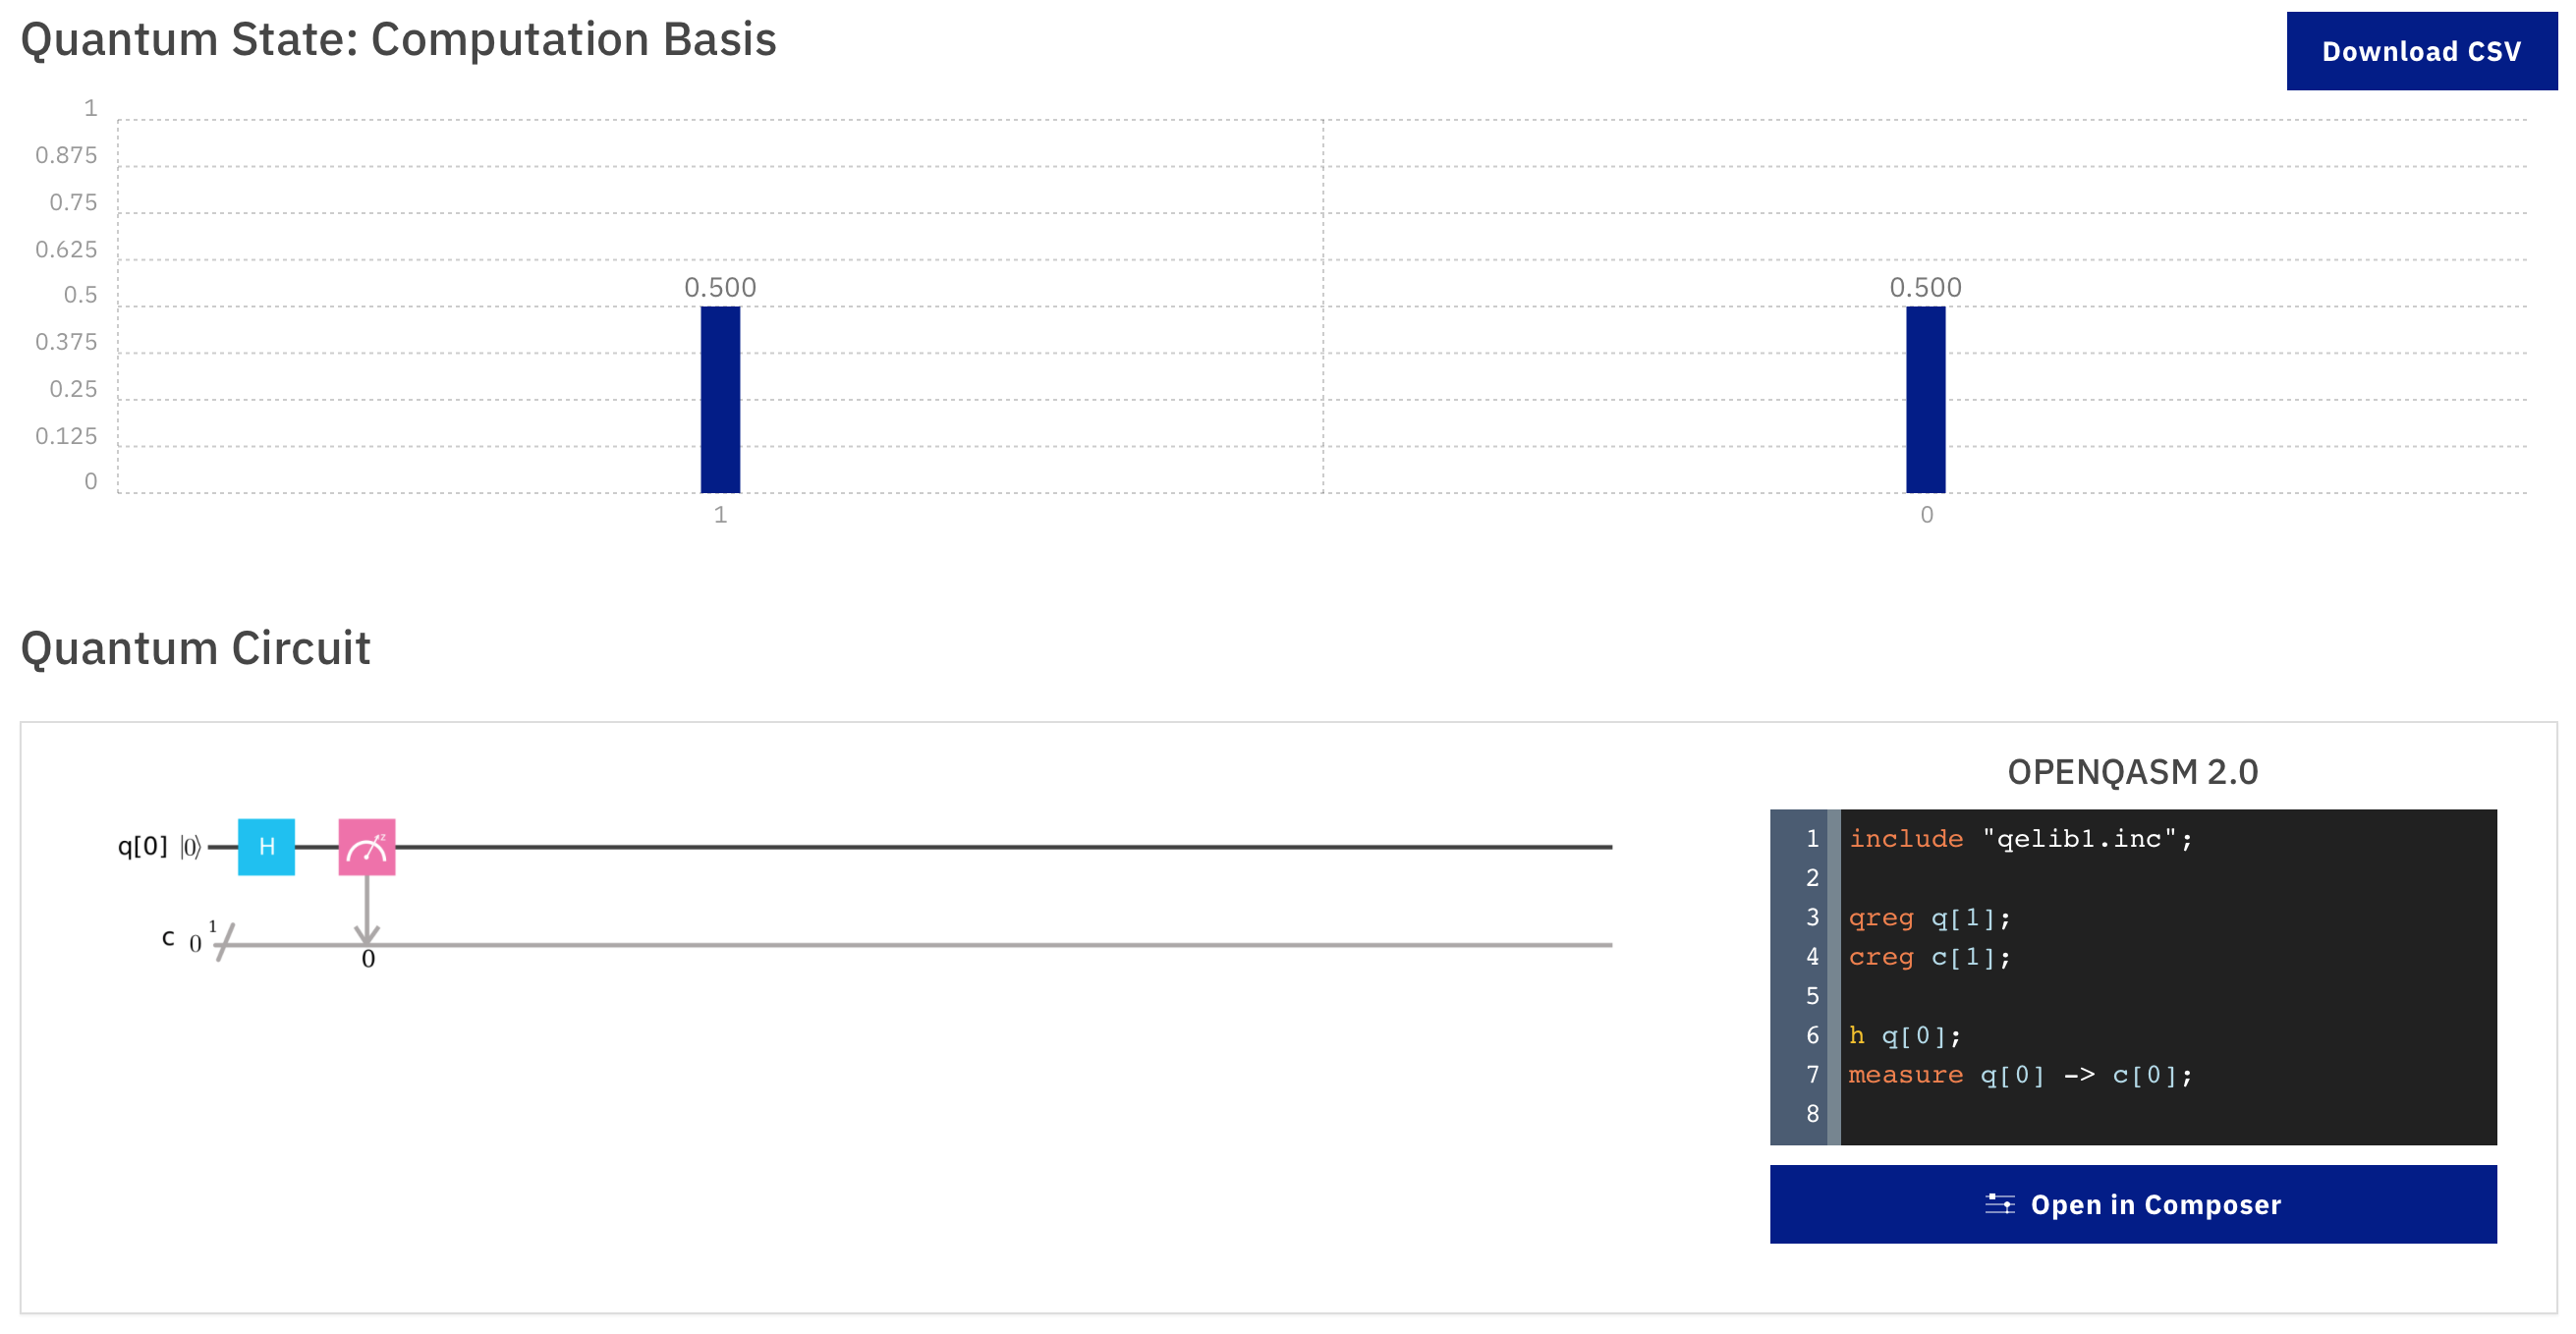
\includegraphics[width=4.2in]{images/ibmQuantumSphereHadamard.png}
\caption{Display of Hadamard port applied to input $|0\rangle$: the output is $|\psi\rangle = |0\rangle + |1\rangle$.}
\label{ibmQuantumSphereHadamard}
\end{center}
\end{figure}

The effect of $H$ can therefore be seen as an \textit{half-executed} \texttt{NOT}, so that the resulting state is neither $0$ nor $1$, but a coherent overlap of the two base states. For this reason $H$ is often called the \textit{square root of} \texttt{NOT}. Note that this expression has \textbf{only} a physical meaning! From an algebraic point of view, $H^2$ is not the $X$ matrix. With a simple calculation one can in fact verify that $H^2$ is the identity and therefore applying $H$ twice to a state leaves it unaltered. In the Bloch sphere, the $H$ operation corresponds to a rotation of $\ang{90}$ of the sphere around the $Y$ axis followed by a reflection through the plane $(X, Z)$. Another way to see the rotation is to imagine it as a $\ang{180}$ rotation over the bisector between $X$ and $Z$ axis: a $\ang{180}$ rotation around $X+Z$ swaps points on the $X$ axis to the $Z$ axis (and vice versa), and negates points on the $Y$ axis. The \autoref{hfig} shows the effect of applying $H$ to qubit $|0\rangle$.

\from{Matteo}{Use Geogebra / replace with IBM doc image to show the transformation.}
\begin{figure}[!htb]
\begin{center}
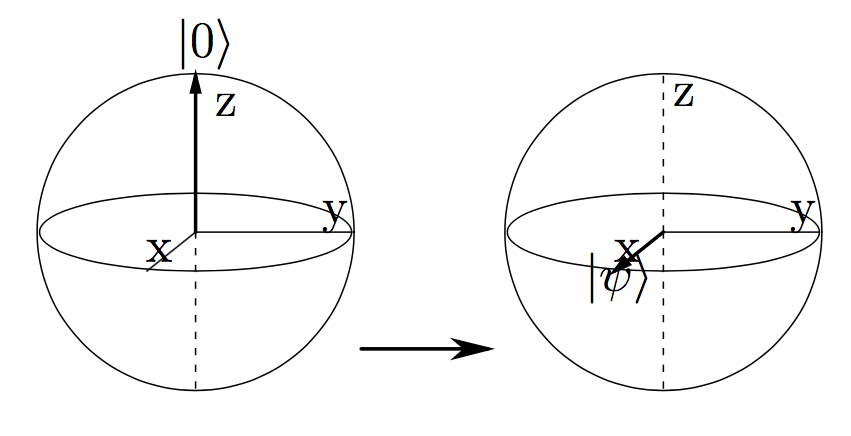
\includegraphics[width=2.5in]{images/hfig.png}
\caption{Display of Hadamard port applied to input $|0\rangle$: the output is $\frac{|0\rangle + |1\rangle}{\sqrt{2}}$.}
\label{hfig}
\end{center}
\end{figure}

You can try to visualize the effect of $H$ on the qubit $$\frac{|0\rangle + |1\rangle}{\sqrt{2}}$$

For effect of the rotation and subsequent reflection through the plane $x, y$ you will obtain again $|0\rangle$.

The logic gates to a qubit $X$, $Z$ and $H$ are represented graphically as in Fig. \ref{qports}.

\begin{figure}[!htb]
\begin{center}
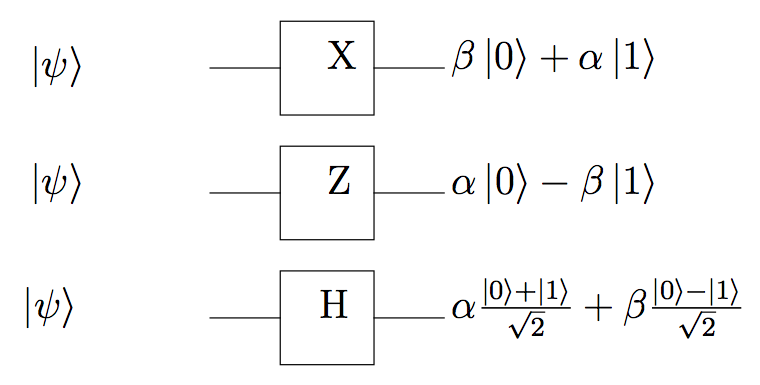
\includegraphics[width=3.0in]{images/qports.png}
\caption{The X, Z and H gates.}
\label{qports}
\end{center}
\end{figure}

\subsection{Multiple qubits quantum logic gates}

\paragraph{} Operations on quantum registers of two or more qubits are necessary to describe the transformations of compound states and in particular of the \textit{so-called} \textbf{entangled states}. We have seen that a two-qubit register can not always be decomposed into the tensor product of the individual qubits components (see definition \ref{entanglement}). Therefore we can not in such cases simulate an operation on the two qubits through operations on each qubit component. Also operations on qubit registers correspond to unit operations as in the case of a single qubit.
The most important logic gates that implement operations on two classic bits are the \texttt{AND}, \texttt{OR}, \texttt{XOR}, \texttt{NAND} and \texttt{NOR} ports. The \texttt{NOT} and \texttt{AND} ports form a universal set, i.e. any boolean function can be accomplished by a combination of these two operations. For the same reason, the \texttt{NAND} constitutes a universal whole. Note that \texttt{XOR} alone or even together with \texttt{NOT} is not universal: since it preserves the total parity of the bits, only a subset of the boolean functions can be represented by this operation.
The quantum analog of \texttt{XOR} is the \texttt{CNOT} gate (controlled-\texttt{NOT}) which operates on two qubits: the first is called the control qubit and the second is the qubit target. The \texttt{CNOT} gate is graphically represented by the circuit in Fig. \ref{cnot}.
\begin{figure}[!htb]
\begin{center}
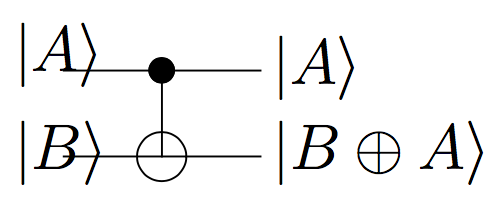
\includegraphics[width=1.5in]{images/cnot.png}
\caption{The \texttt{CNOT} gate.}
\label{cnot}
\end{center}
\end{figure}

If the control is zero then the target is left unchanged; if the control is one, then the target is denied, that is
$$|00\rangle \rightarrow{} |00\rangle, |01\rangle \rightarrow{} |01\rangle, |10\rangle \rightarrow{} |11\rangle, |11\rangle \rightarrow{} |10\rangle$$

Equivalently, \texttt{CNOT} can be seen as the transformation
$$|A,B\rangle \mapsto |A,B\rangle \otimes A$$
where $A$ is the control qubit, $B$ is the target and $\otimes$ is the sum module $2$ - that is the classical \texttt{XOR} operation. The representation as a unitary matrix is:
$$\begin{bmatrix}
1 & 0 & 0 & 0 \\
0 & 1 & 0 & 0 \\
0 & 0 & 0 & 1 \\
0 & 0 & 1 & 0
\end{bmatrix}$$
where the first column describes the transformation of the vector of the computational base $|00\rangle$, the second that of the vector $|01\rangle$, the third of $|10\rangle$ and the fourth of $|11\rangle$.
\paragraph{Exercise} Look at exercise 17 in \autoref{exs}.

\paragraph{} It is important to note that the \texttt{CNOT}, like all unit transformations, is invertible: input can always be obtained from the output. This is not true for the \texttt{XOR} and \texttt{NAND} logic gates: in general, classic operations are irreversible.
The \texttt{CNOT} gate and one-qubit ports represent the prototypes of all quantum logic gates. In fact, is is possible to demonstrate the universality of these operations (later on this).

\subsubsection{IBM Q - Testing the \texttt{CNOT} gate}

\from{Matteo}{Add experiment over this.}

\paragraph{} The gates made with vertical lines connecting two qubits together are a physical implementation of the \texttt{CNOT} gates just introduced. These two-qubit gates function like an exclusive \texttt{OR} gate in conventional digital logic. The qubit at the solid-dot end of the \texttt{CNOT} gate controls the whether or not the target qubit at the $\oplus$-end of the gate is inverted (hence \texttt{controlled NOT}, or \texttt{CNOT}). Some gates, like the \texttt{CNOT}, have hardware constraints; the set of allowed connections is defined by the schematic of the device located below the quantum Composer, along with recently calibrated device parameters.

\newpage

\section{Quantum circuits}

\subsection{SWAP operation}

\paragraph{} A simple example of a quantum circuit is given in Fig. \ref{circuit}. 
\begin{figure}[!htb]
\begin{center}
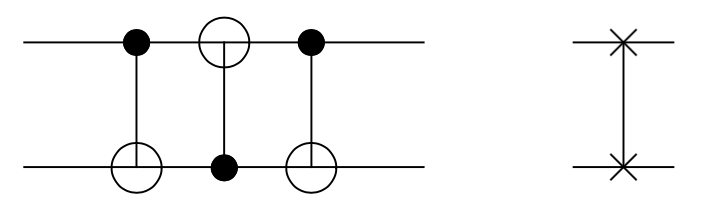
\includegraphics[width=3.0in]{images/circuit.png}
\caption{Circuit that exchanges two qubits and a schematic symbol.}
\label{circuit}
\end{center}
\end{figure}

The circuit realizes the exchange of two qubits states. Given in input the register of two qubits $|a, b\rangle$, a \texttt{CNOT} is carried out with qubit of control a. As a result, $b$ is replaced by $a \otimes b$. The latter is taken as a control of a second \texttt{CNOT} with target $a$. The effect is that a is replaced by $a \otimes (a \otimes b) = b$. Finally, a last \texttt{CNOT} with control $b$ and target $a \otimes b$ realizes the exchange by replacing $a \otimes b$ with $a$. Given any unit operation $U$ on $n$ qubits, the controlled-$U$ circuit can be defined as the natural extension of the \texttt{CNOT} gate (see Fig. \ref{controlledu}). 
\begin{figure}[!htb]
\begin{center}
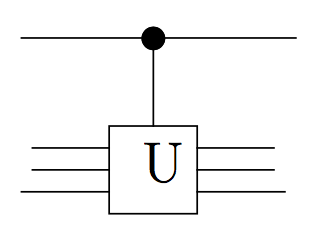
\includegraphics[width=1.5in]{images/controlledu.png}
\caption{Controlled-U gate.}
\label{controlledu}
\end{center}
\end{figure}

The line with the black dot indicates the control qubit, while the qubits target are the $n$ inputs of $U$. According to this convention the controlled-\texttt{NOT} is nothing more than a controlled-$U$ with $U = X$.

Another important operation is represented by the symbol in Fig. \ref{mesured}.
\begin{figure}[!htb]
\begin{center}
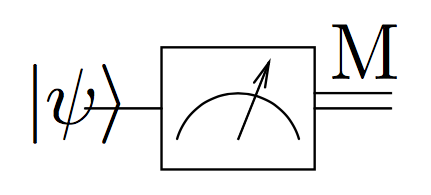
\includegraphics[width=1.5in]{images/mesured.png}
\caption{Circuit symbol for measurement.}
\label{mesured}
\end{center}
\end{figure}

\paragraph{} Testing the swapping of the qubit is really simple. Let's prepare a simulated register with two qubit in the initial state $|10\rangle$, like the one shown in \autoref{fig:quantumSwap}.

\begin{figure}[!htb]
\begin{center}
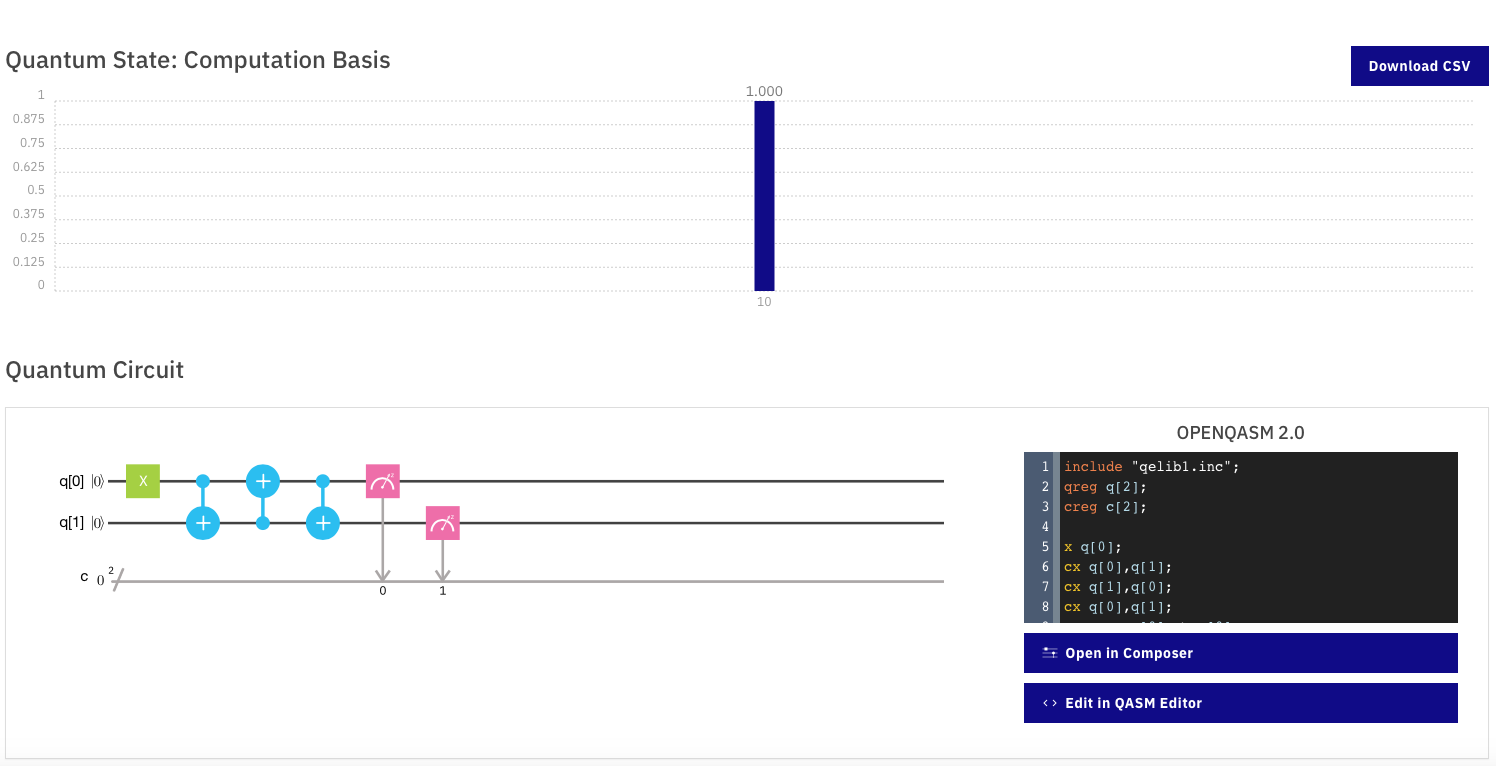
\includegraphics[width=4.5in]{images/quantumSwap.png}
\caption{Circuit for swapping two qubit state.}
\label{fig:quantumSwap}
\end{center}
\end{figure}
\textbf{NOTE}: in \textit{IBM} platform the histogram will provide the result in the opposite order. For instance, in the figure, the unique bar on histogram is labelled $10$, where $1$ refer to the second (\texttt{q[1]}) qubit in the register and $0$ to the first (\texttt{q[0]}). Thus, as show in the histogram, the result will be the swapping between the two qubit. Mathematically, the proof is simple. Let's start by saying that
$$|0\rangle = \binom{1}{0}$$
Thus, 
$$X|0\rangle = \binom{1}{0}\left({\begin{matrix} 0 & 1 \\ 1 & 0 \\ \end{matrix}}\right)$$
The initial state is ready (with value $|10\rangle$). Then, we apply a \texttt{CNOT}. Our first qubit is in $|1\rangle$, thus the second qubit will be negated as well: the status become $|11\rangle$. Then, a second \texttt{CNOT} is applied using the second qubit as a control and the first as a target qubit. The first qubit change to the $|0\rangle$, bringing the entire register in the $|01\rangle$. The last \texttt{CNOT} doesn't anything: the swap is completed. Ok but what if the initial status was set tup $|00\rangle$ or any other possible permutation? Let's see the effect of the circuit over the four possible initial state (the third is the one we already described).
$$|00\rangle \xrightarrow{\ang{1} \; CNOT} |00\rangle \xrightarrow{\ang{2} \; CNOT} |00\rangle \xrightarrow{\ang{3} \; CNOT} |00\rangle$$

$$|01\rangle \xrightarrow{\ang{1} \; CNOT} |01\rangle \xrightarrow{\ang{2} \; CNOT} |11\rangle \xrightarrow{\ang{3} \; CNOT} |10\rangle$$

$$|10\rangle \xrightarrow{\ang{1} \; CNOT} |11\rangle \xrightarrow{\ang{2} \; CNOT} |01\rangle \xrightarrow{\ang{3} \; CNOT} |01\rangle$$

$$|11\rangle \xrightarrow{\ang{1} \; CNOT} |10\rangle \xrightarrow{\ang{2} \; CNOT} |10\rangle \xrightarrow{\ang{3} \; CNOT} |11\rangle$$

\subsection{No-cloning}

\paragraph{} Is it possible to build a circuit that makes a copy of a qubit? You could think of using a \texttt{CNOT} with control qubit containing the qubit $|x\rangle$ to be copied and the target initially set to $|0\rangle$. The result would be the copying of $x$ in the target. In reality this is true for classic bits (or for the states of the computational basis) but not for a generic qubit $|\psi\rangle = a|0\rangle + b|1\rangle$. In fact, let's consider the circuit in \autoref{noCloning}, consisting of a \texttt{CNOT} that has as input the qubits $|\psi\rangle$ (control) and $|0\rangle$ (target), i.e. the register $|\psi\rangle |0\rangle$.
Our goal is to get the result $|\psi\rangle |\psi\rangle$. We observe that:
$$|\psi\rangle|\psi\rangle = a^2|00\rangle + ab|01\rangle + ab|10\rangle + b^2|11\rangle$$
This is due to the nature of a register, that is a tensor product between vectors of respective qubit. Thus, 
$$|\psi\rangle|\psi\rangle = (a|0\rangle + b|1\rangle) * (a|0\rangle + b|1\rangle) = a^2|00\rangle + ab|01\rangle + ab|10\rangle + b^2|11\rangle$$

\paragraph{Theorem} The point is that there is no unit transformation $M$ such that $M$ $|\psi\rangle$ $|0\rangle$ = $|\psi\rangle$ $|\psi\rangle$, for each state $|\psi\rangle$.

\begin{figure}[!htb]
\begin{center}
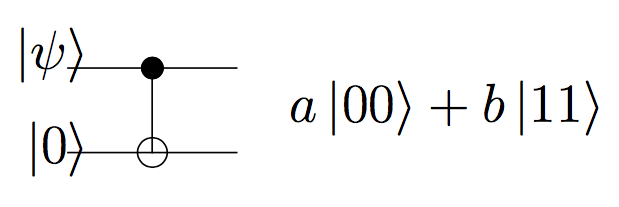
\includegraphics[width=1.5in]{images/noCloning.png}
\caption{Quantum circuit that can not ``copy" a qubit.}
\label{noCloning}
\end{center}
\end{figure}

\subsubsection{Proof} Suppose that there exists $M$ such that $M|\psi\rangle|0\rangle = |\psi\rangle|\psi\rangle$, for each qubit $|\psi\rangle$. Then we can choose two qubits $|\psi\rangle$ and $|\phi\rangle$ such that $$0 < \langle\psi|\phi\rangle < 1$$

For instance, we can take
$$|\psi\rangle = |0\rangle \; \; and \; \; |\phi\rangle = \frac{|0\rangle + |1\rangle}{\sqrt{2}}$$ 

Because $M$ exists, then:
$$M |\psi\rangle |0\rangle = |\psi\rangle |\psi\rangle$$

and
$$M |\phi\rangle |0\rangle = |\phi\rangle |\phi\rangle$$

Let's now do the scalar product (between each member) of the two equations. Since $M$ is unitary and therefore preserves the scalar products (see Exercise 4.7), and for the distributive property of the tensor product with respect to the scalar product (see Exercise 3.4 Lesson 1) we obtain that $\langle\psi|\phi\rangle = \langle\psi|\phi\rangle \langle0|0\rangle = \langle\psi|\phi\rangle$, contradicting the hypothesis that $0 < \langle\psi|\phi\rangle < 1$. So $M$ can not exist.

\subsection{Examples of quantum circuits}

\paragraph{} We describe two circuits a little more complicated than those seen previously: the first allows to transform the four computational states of two qubits into many states that are called \texttt{Bell states} or \texttt{EPR} pairs; the second uses these states to realize the teleportation of a qubit. These two examples show how to construct computational states that do not have any classical counterparts and use them to give rise to paradoxical phenomena according to the laws of classical physics. These states are those we have called entangled.

\subsubsection{Bell states}
We have seen that the \texttt{CNOT} gate can be used to create states that are entangled. The circuit in \autoref{bellCircuit} generates a particular entangled state for each state of the computational base $|00\rangle$, $|01\rangle$, $|10\rangle$, $|11\rangle$. These states, which we indicate with $\beta00$, $\beta10$, $\beta10$, $\beta1$ are called Bell or EPR states by Bell, Einstein, Podolsky and Rosen who first discovered their extraordinary properties. In particular, Einstein, Podolsky and Rosen used these states in an experiment that in their intentions had to show that quantum mechanics was not able to give a complete description of reality. The paradox that came out of this experiment was that the interaction between these pairs of quantum states gave rise to a phenomenon that violated the fundamental principles of the theory of relativity. The ``classical" explanation that they proposed was later disproved by Bell.
\begin{figure}[!htb]
\begin{center}
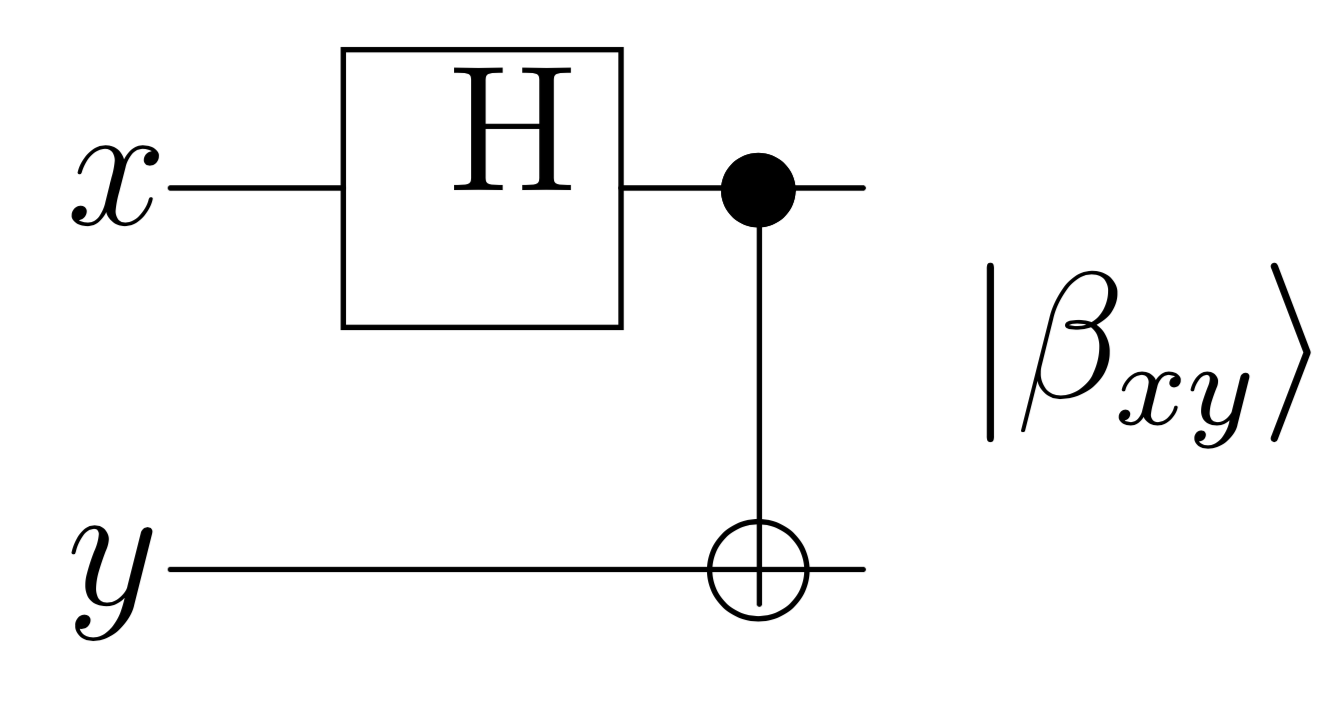
\includegraphics[width=1.5in]{images/bellCircuit.png}
\caption{Quantum circuit to create the Bell states.}
\label{bellCircuit}
\end{center}
\end{figure}

The circuit transforms the first qubit into an overlap that is then used as control input for \texttt{CNOT}. The target is then inverted only when the control is 1. Therefore the input vectors are transformed as follows:
\begin{equation}
\begin{split}
|00\rangle \mapsto |\beta_{00} \equiv (|00\rangle + |11\rangle) / \sqrt{2} \\
|01\rangle \mapsto |\beta_{01} \equiv (|01\rangle + |10\rangle) / \sqrt{2} \\
|10\rangle \mapsto |\beta_{10} \equiv (|00\rangle - |11\rangle) / \sqrt{2} \\
|11\rangle \mapsto |\beta_{11} \equiv (|01\rangle - |10\rangle) / \sqrt{2}
\end{split}
\label{eq:bellStates}
\end{equation}

\subsubsection{Quantum teleportation}

\paragraph{} Quantum teleportation is a technique for transporting quantum states from one place to another by exploiting only the transmission of classical bits. This technique was discovered in 1993 and its validity was then confirmed by various experimental results. One of the first experiments that marked an enormous progress in the study of this technique was carried out at the University of Geneva (see Nature No. 421 of January 30, 2003) and carried out the teleportation of a qubit between two laboratories located 55 meters away. exploiting a standard telecommunication channel of 2 Km. Since then, enormous progress has been made which continues to follow each other with increasing frequency. The journal Nature has recently published (see No. 489 of September 13, 2012) an article by Anton Zeilinger and his team of the Institute for Quantum Optics and Quantum Information in Vienna where it is reported as an experiment allowed the team to teleport photons at a distance of about 143 km between the two islands of the Canary Islands La Palma and Tenerife.

To understand the type of problems that teleportation can solve, we imagine a situation in which a person we call Alice must make the status of a qubit known to another person we will call Bob. Alice does not know the status of the qubit and for the no-cloning theorem we know that it is not possible to make a copy of it. In addition, Alice can only send Bob classic information, that is, the values 0 and 1 of a classic bit. In this situation it would be impossible to transmit the qubit to Bob. Let's see how it is possible thanks to the properties of the entangled states.

The basic hypothesis is that Bob and Alice each have a qubit of a previously generated \texttt{EPR} pair - that is one of the four entangled state generated by the circuit shown in \autoref{bellCircuit}. This pair is identified by the sort of bracket near the Bell pair $\beta_{00}$. Alice can work on her qubit and Bob can do the same on his part of the \texttt{EPR} pair. The circuit in \autoref{quantumTeletrasportation} illustrates the transmission of a qubit 
$$|\psi\rangle = \alpha|0\rangle + \beta|1\rangle$$

whose amplitudes $\alpha$ and $\beta$ are unknown, from Alice to Bob. The input state of the circuit is
$$|\psi_0\rangle = |\psi\rangle|\beta_{00}$$

\begin{figure}[!htb]
\begin{center}
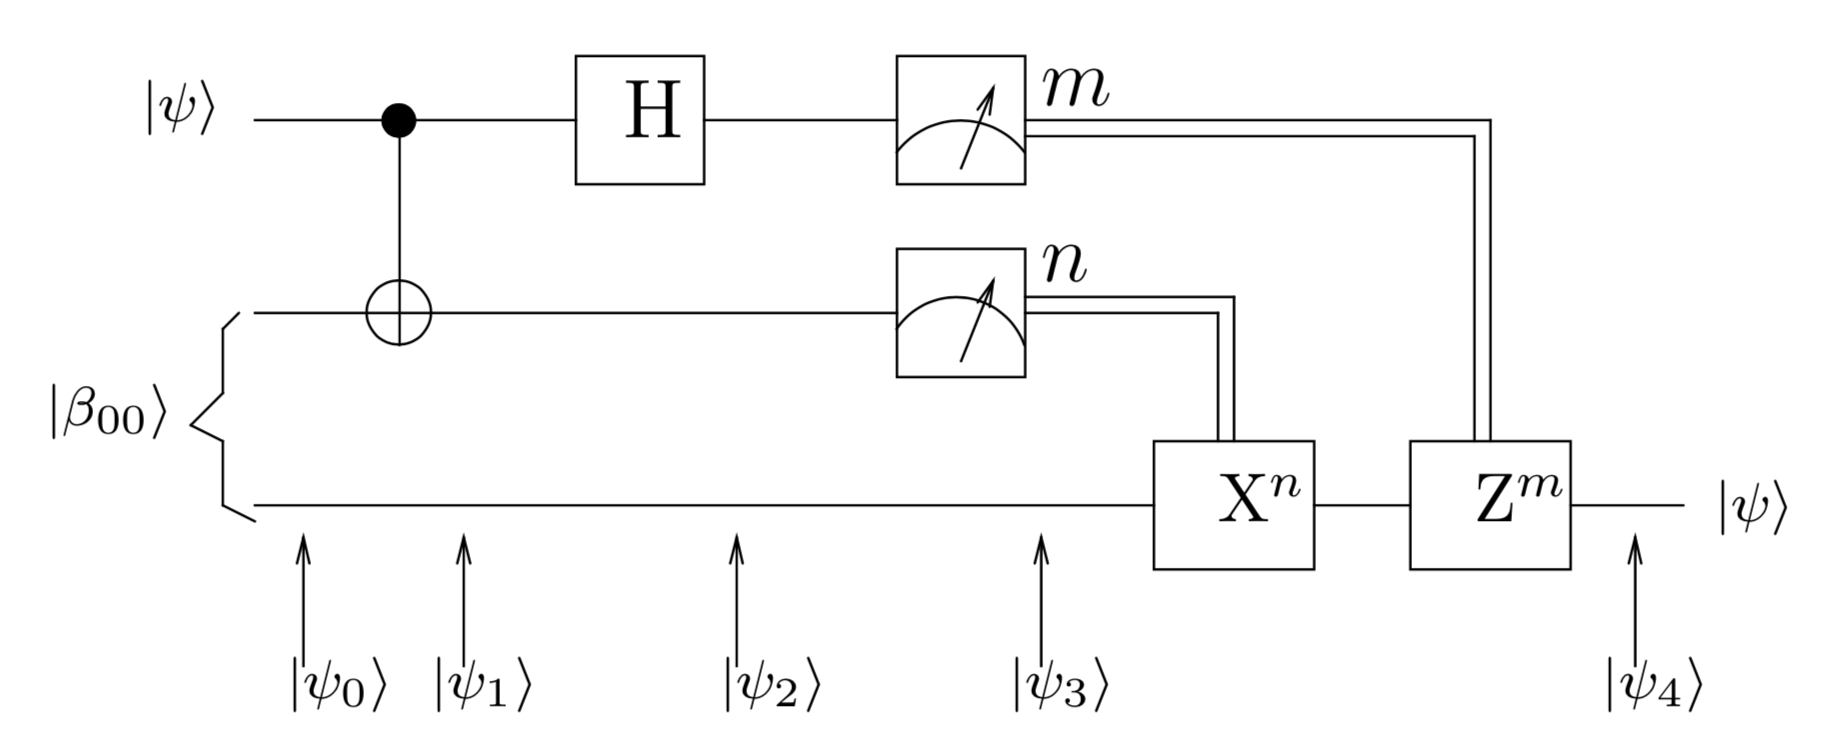
\includegraphics[width=4.0in]{images/quantumTeletrasportation.png}
\caption{Quantum circuit for teleportation of a qubit.}
\label{quantumTeletrasportation}
\end{center}
\end{figure}

Alice combines $|\psi_0\rangle$ with her half of the \texttt{EPR} pair and measures her two qubits after applying the \texttt{CNOT} and \texttt{Hadamard} ports. The two bits that gets after the measurement are sent through a classic communication channel to Bob, who will be able to reconstruct the $|\psi\rangle$ state using the classic information received from Alice and her half of the \texttt{EPR} pair.

In the circuit shown in the figure, the first two lines correspond to the qubits used by Alice, while the last line corresponds to the qubit owned by Bob. The input is
\begin{equation*}
\begin{split}
|\psi_0\rangle & = |\psi\rangle |\beta_{00}\rangle = \\  & = (\alpha|0\rangle + \beta|1\rangle) \frac{(|00\rangle + |11\rangle)}{\sqrt{2}} = \\
 & = \frac{1}{\sqrt{2}}\left[\alpha|0\rangle \left(|00\rangle + |11\rangle\right) + \beta|1\rangle \left(|00\rangle + |11\rangle\right) \right] = \\
 & = \frac{1}{\sqrt{2}}\left[\alpha|000\rangle + \alpha|011\rangle + \beta|100\rangle + |111\rangle\right]
\end{split}
\end{equation*}

where the state $|\beta_{00} \equiv (|00\rangle + |11\rangle) / \sqrt{2}$ occupies the second qubit of Alice and the qubit of Bob. Have a look at the last line: if a \texttt{CNOT} is applied to the first qubit, then the second qubit will change state and will be the opposite of the control qubit. As a result of \texttt{CNOT} applied to its two qubits (the first two qubits), Alice gets:

\begin{equation*}
\begin{split}
|\psi_1\rangle & = \frac{1}{\sqrt{2}}\left[\alpha|0\rangle \left(|00\rangle + |11\rangle\right) + \beta|1\rangle \left(|10\rangle + |01\rangle\right) \right] \\
 & = \frac{1}{\sqrt{2}}\left[\alpha|000\rangle + |011\rangle + \beta|110\rangle + |101\rangle\right]
\end{split}
\end{equation*}

The first two possible final configuration remain equals because they represent the scenario in which the first qubit (control) collapse to $0$, so they remain $00$ and $11$, providing the two possible configuration $\alpha|000\rangle$ and $\alpha|011\rangle$. The second two final configurations change because the \texttt{CNOT} applied to the value of the first qubit, if it collapse to 1, will make the negation of the value of the second qubit. So the second two final states after the \texttt{CNOT} application become $\alpha|110\rangle$ and $\alpha|101\rangle$ with the first 1 that change the second qubit to 0 and the the second qubit 1, respectively, in the two final configurations.

Then Hadamard is applied to the first qubit, $|\psi\rangle$, that is still in the state $$|\psi\rangle = \alpha|0\rangle + \beta|1\rangle$$

because no effective measure was done on that. So 

Remember that Hadamard applied to the $|\psi\rangle = \alpha|0\rangle + \beta|1\rangle$, as shown in \autoref{qports}, give
\begin{equation*}
H(|\psi\rangle) = \alpha\frac{|0\rangle + |1\rangle}{\sqrt{2}} + \beta\frac{|0\rangle - |1\rangle}{\sqrt{2}}
\end{equation*}

So, if you apply \texttt{H} to $|\psi_1\rangle$, you get
\begin{equation*}
\begin{split}
|\psi_2\rangle & = \frac{1}{\sqrt{2}}\left[\alpha(|0\rangle + |1\rangle) \left(|00\rangle + |11\rangle\right) + \beta(|0\rangle - |1\rangle) \left(|10\rangle + |01\rangle\right) \right] \\
 & = \frac{1}{\sqrt{2}}(\alpha(|0\rangle + |1\rangle) \left(|00\rangle + |11\rangle\right) + \beta(|0\rangle - |1\rangle) \left(|10\rangle + |01\rangle\right)) \\
 & = \frac{1}{\sqrt{2}}(\alpha|000\rangle + \alpha|011\rangle + \alpha|100\rangle + \alpha|111\rangle + \\ 
 & + \; \; \; \; \; \; \; \; \beta|010\rangle + \beta|001\rangle - \beta|110\rangle - \beta|101\rangle) \\
\end{split}
\end{equation*}

Or, equivalenty

\begin{equation*}
\begin{split}
|\psi_2\rangle & = \frac{1}{\sqrt{2}}\left[\alpha(|0\rangle + |1\rangle) \left(|00\rangle + |11\rangle\right) + \beta(|0\rangle - |1\rangle) \left(|10\rangle + |01\rangle\right) \right] \\
 & = \frac{1}{\sqrt{2}}(|00\rangle(\alpha|0\rangle + \beta|1\rangle) + |01\rangle(\alpha|1\rangle + \beta|0\rangle) + \\
 & + \; \; \; \; \; \; \; \; |10\rangle(\alpha|0\rangle - \beta|1\rangle) + |11\rangle(\alpha|1\rangle - \beta|0\rangle)) \\
 & = \frac{1}{\sqrt{2}}(\alpha|000\rangle + \beta|001\rangle + \alpha|011\rangle +  \beta|010\rangle + \\
 & - \; \; \; \; \; \; \; \; \alpha|100\rangle - \beta|101\rangle + \alpha|111\rangle -
 \beta|110\rangle) \\
\end{split}
\end{equation*}

At this point Alice measures her two qubits obtaining one of the four pairs of bits:
$$00 \; \; 01 \; \; 10 \; \; 11$$

As a result of the measurement, Bob's qubit will also collapse in the state corresponding to the measurement result, i.e.:
\begin{equation*}
\begin{split}
00 \mapsto \alpha|0\rangle + \beta|1\rangle \\
01 \mapsto \alpha|1\rangle + \beta|0\rangle \\
10 \mapsto \alpha|0\rangle - \beta|1\rangle \\
11 \mapsto \alpha|1\rangle - \beta|0\rangle \\
\end{split}
\end{equation*}

In the \autoref{quantumTeletrasportation}, this state is indicated with $|\psi_3\rangle$. Alice communicates the two bits $m$ and $n$ obtained to Bob through a classic channel. Bob is now able to get the qubit $|\psi\rangle$ by applying to his part of the entangled Bell state the following transformation:
\begin{table}[!htb]
\centering
\begin{tabular}{|c|c|c|c|c|c|}
\hline
m & n & Gate \\ \hline
0 & 0 & \texttt{I} \\ \hline
0 & 1 & \texttt{X} ($\sigma_x$) \\ \hline
1 & 0 & \texttt{Z} ($\sigma_z$) \\ \hline
1 & 1 & \texttt{ZX} ($i\sigma_y$) \\ \hline
\end{tabular}
\caption{Bob applications}
\label{bobTeleportGates}
\end{table}

This in \autoref{quantumTeletrasportation} is identified by the notation \texttt{$X^n$} and \texttt{$Z^m$}, where \texttt{$X^n$} with $n$ implies do not apply \texttt{X} and the same for \texttt{Z}. Remember that
\begin{equation*}
\begin{aligned}
X = \begin{bmatrix}
0 & 1 \\
1 & 0 \\
\end{bmatrix} \; \; \; 
Y = \begin{bmatrix}
0 & i \\
-i & 0 \\
\end{bmatrix} \; \; \;
Z = \begin{bmatrix}
1 & 0 \\
0 & -1 \\
\end{bmatrix}
\end{aligned}
\end{equation*}
Thus,
\begin{equation*}
\begin{aligned}
i\sigma_y = i\begin{bmatrix}
0 & i \\
-i & 0 \\
\end{bmatrix} \; \; \;
\begin{bmatrix}
0 & -1 \\
+1 & 0 \\
\end{bmatrix}
\end{aligned}
\end{equation*}
That is equivalent to
\begin{equation*}
\begin{aligned}
iXZ = i\begin{bmatrix}
0 & 1 \\
1 & 0 \\
\end{bmatrix} = 
\begin{bmatrix}
1 & 0 \\
0 & -1 \\
\end{bmatrix} = 
\begin{bmatrix}
0+0 & 0-1 \\
1+0 & 0+0 \\
\end{bmatrix}
\end{aligned}
\end{equation*}

\subsubsection{IBM Q - Testing Quantum teleportation}

\paragraph{} In the next paragraph is described the circuit to test the quantum teleportation using the \texttt{IBM Q} platform. You can use the OpenQASM 2.0 (specification of language in \cite{qasm2}) to define a state $|\psi\rangle$ to transfer. I prepared a state following the same procedure in \cite{teleportationUnderExp}: the OpenQASM 2.0 code to do that is in \autoref{teleportationExample}.
\begin{figure}[!htb]
\begin{center}
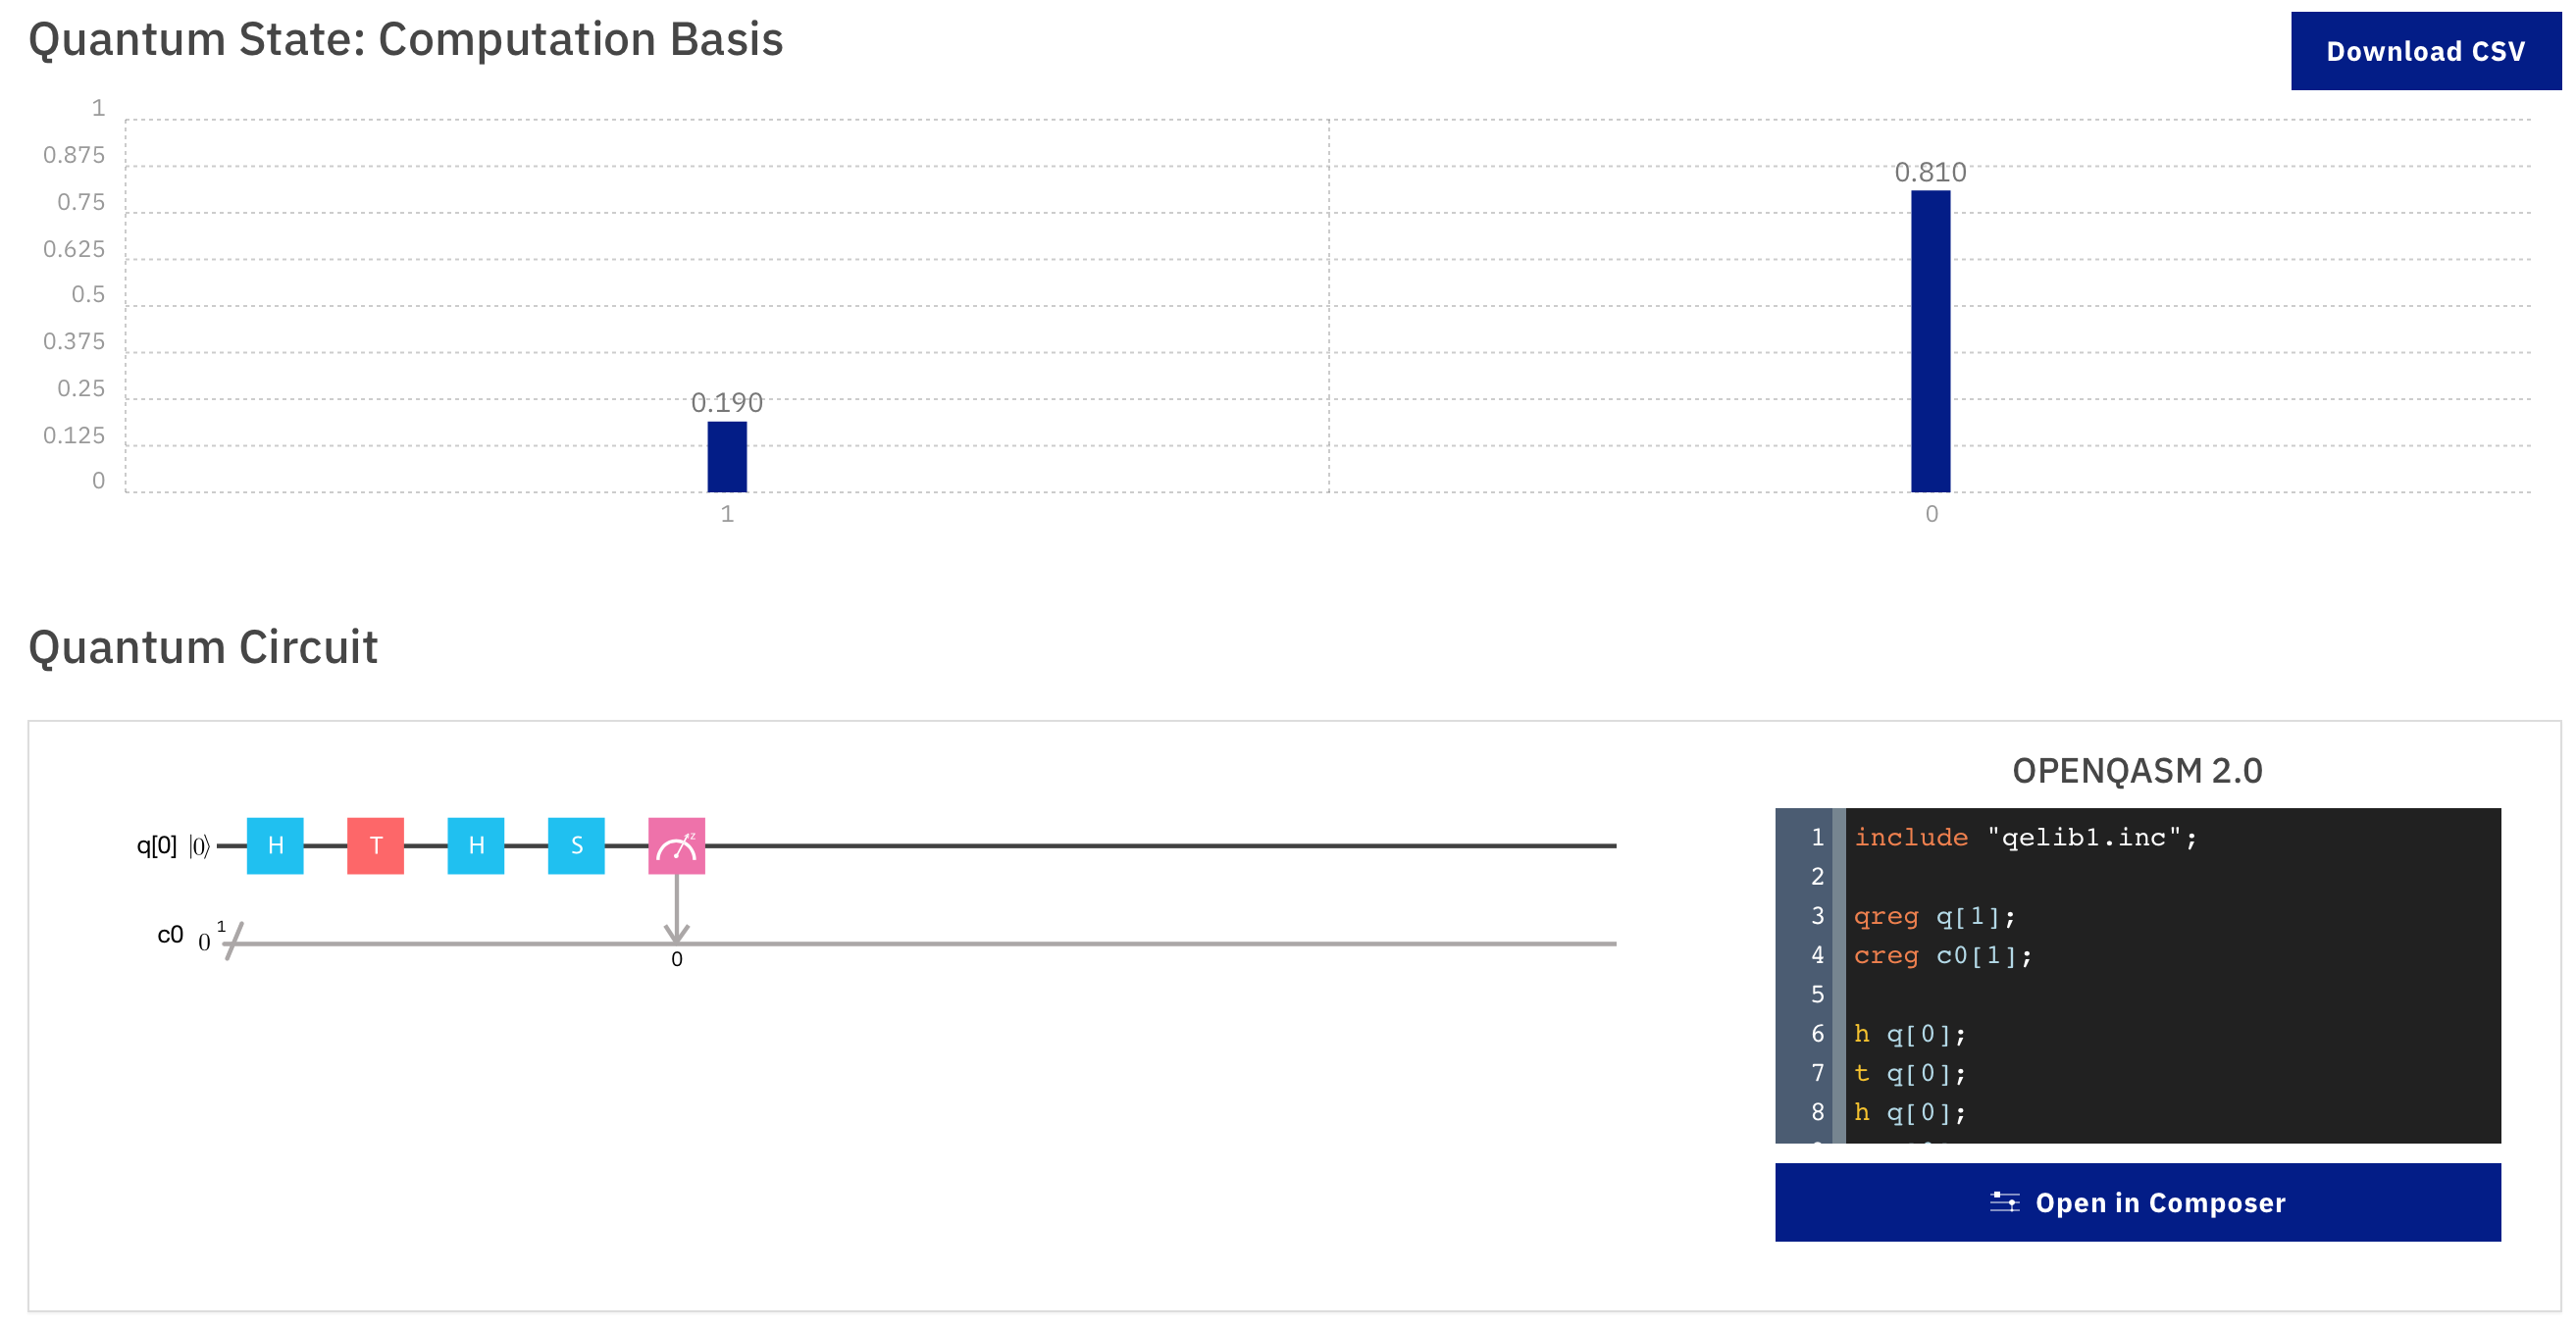
\includegraphics[width=4.5in]{images/teleportationExample.png}
\caption{Quantum circuit to create the state to teleport.}
\label{teleportationExample}
\end{center}
\end{figure}

This state, thanks to the gates applied (all single qubit gates) the prepared state will collapse to $|0\rangle$ in the (quite) $80\%$. The circuit to create teleportation is shown in \autoref{teleportationComplete}.
\begin{figure}[!htb]
\begin{center}
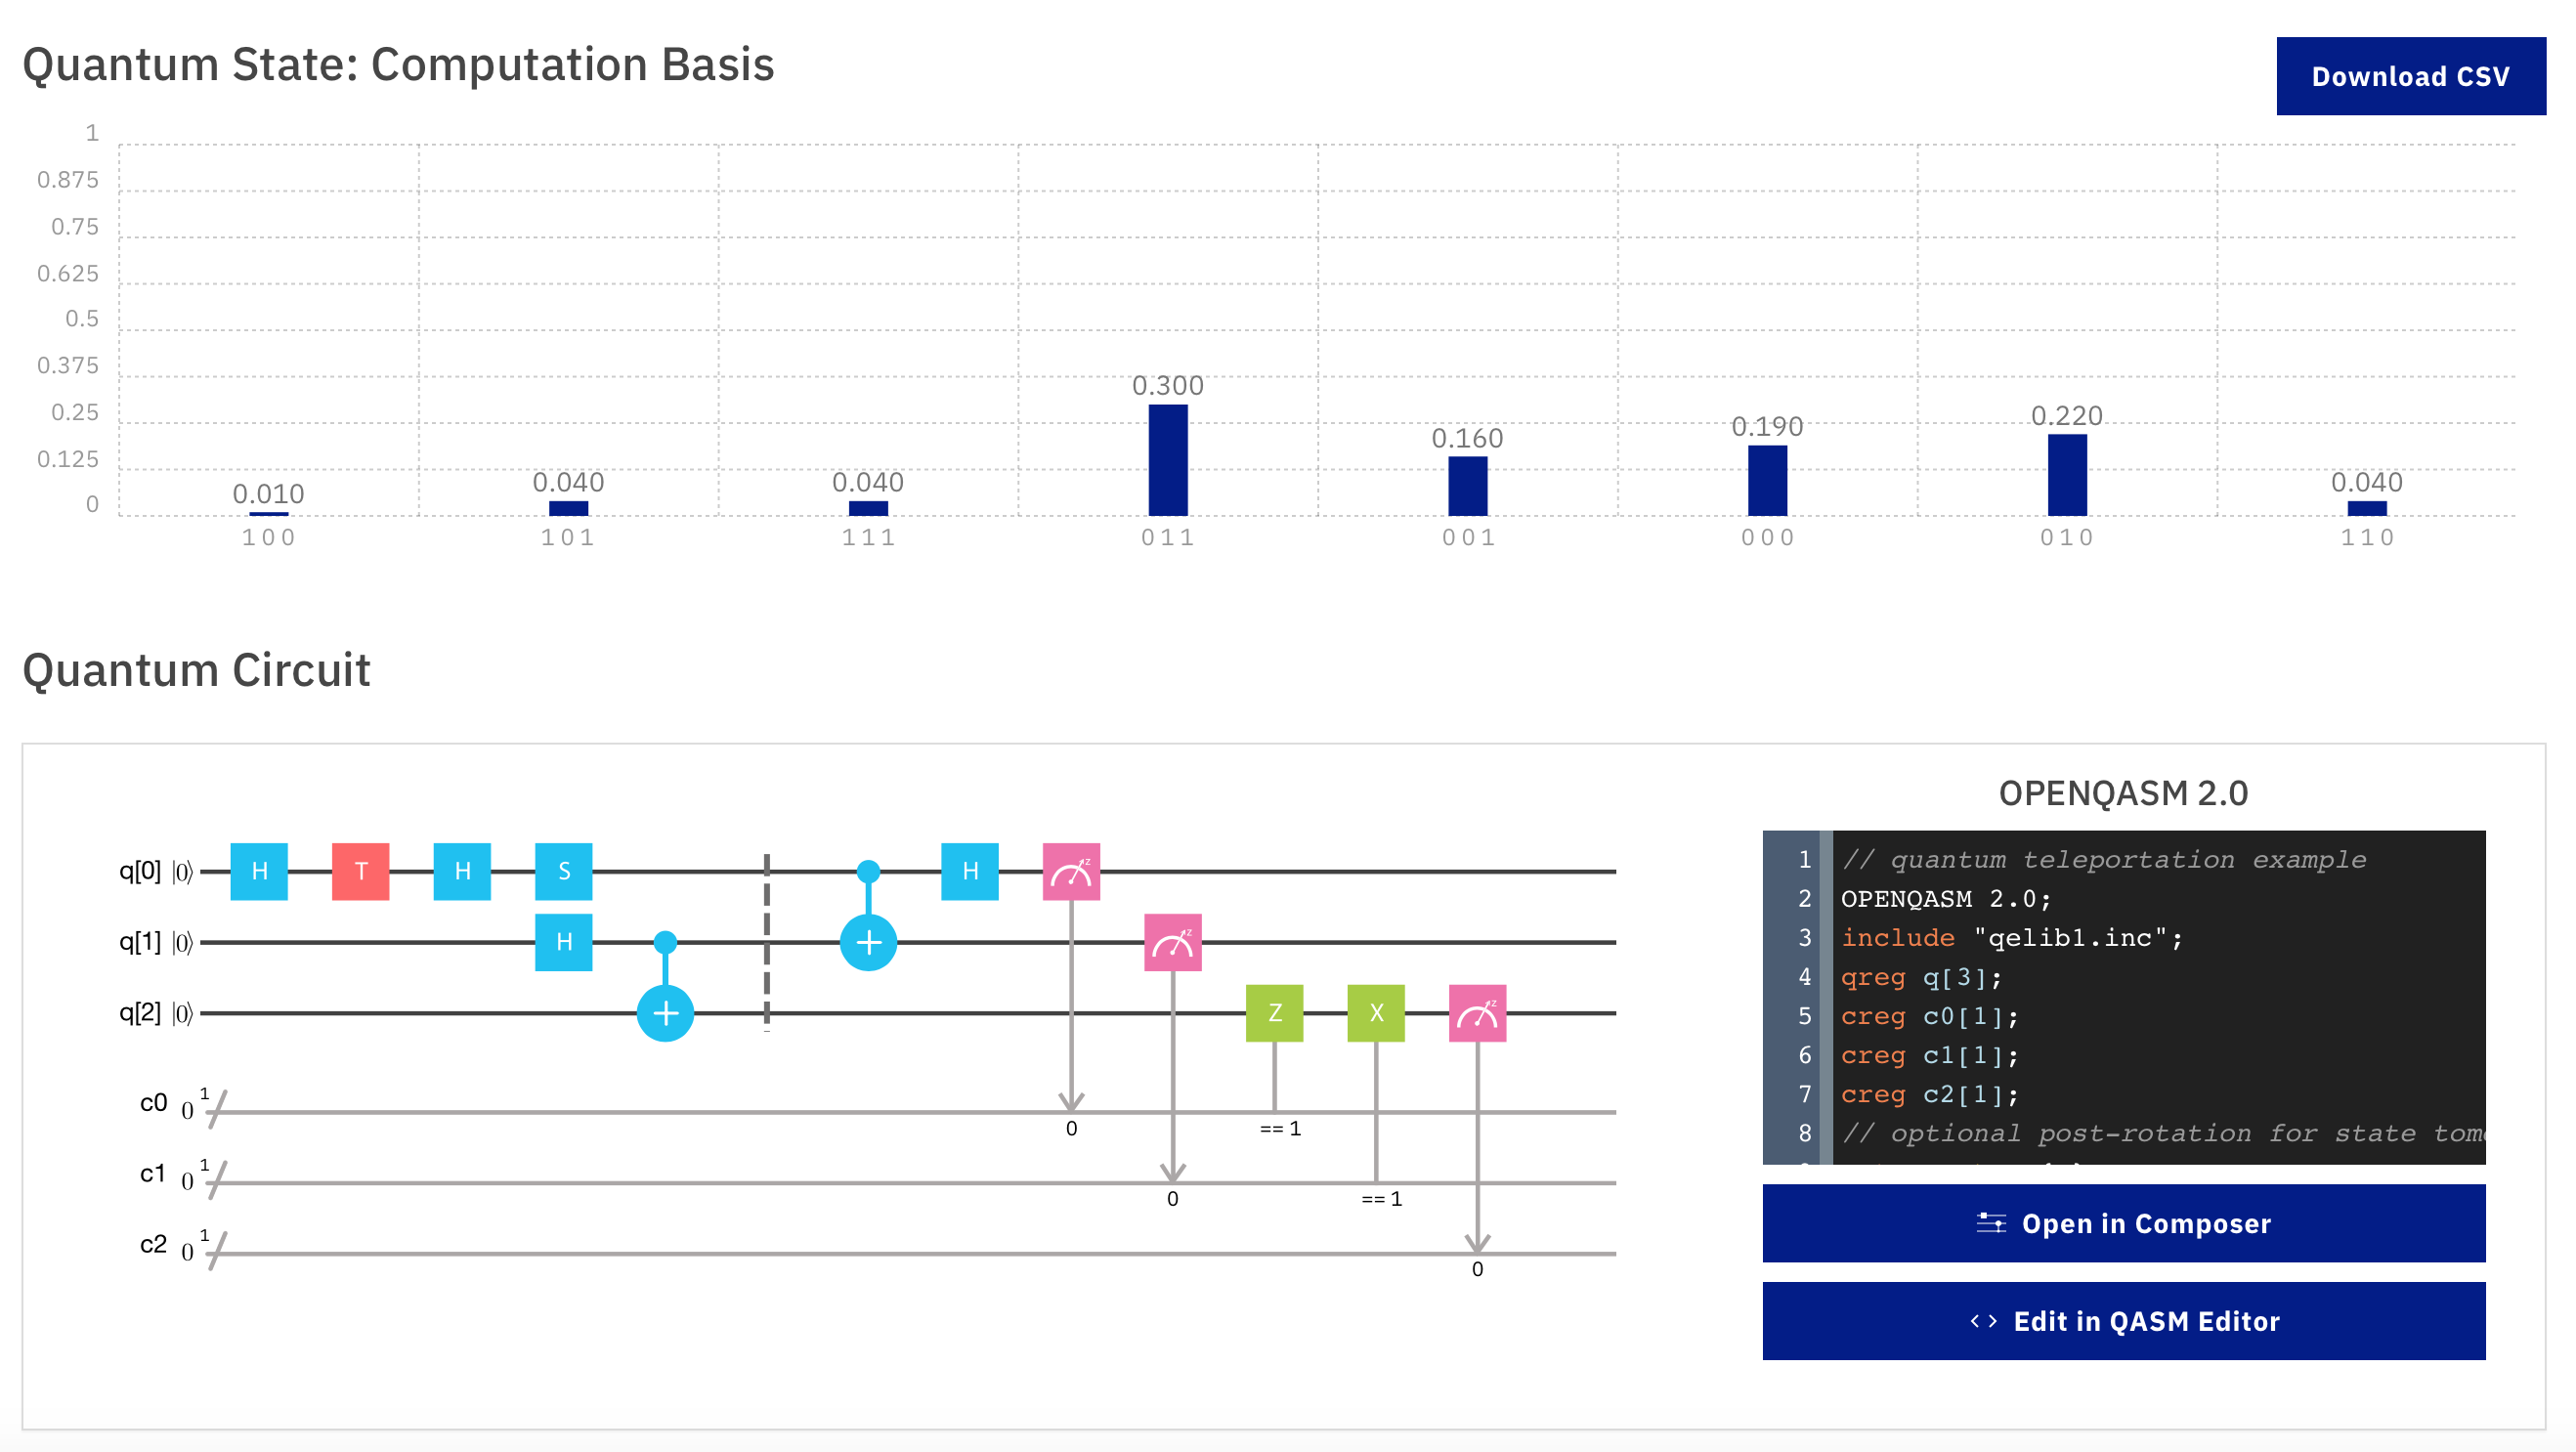
\includegraphics[width=4.5in]{images/teleportationCircuit.png}
\caption{Quantum circuit to create the state to teleport.}
\label{teleportationComplete}
\end{center}
\end{figure}

If you have a look at the \autoref{teleportationExample} and \autoref{teleportationComplete} you confirm the teleportation of $|\psi\rangle$ is correctly completed. In fact, from \autoref{teleportationExample} we know that $|\psi\rangle$ will collapse to $|0\rangle$ in the $80\%$ of the cases. From \autoref{teleportationComplete}, if you look the ``high probability statuses", they are all status in which the second half of the Bell state is collapsed to $|0\rangle$: the status have to be read in the opposite order so $011 \mapsto q_{2}q_{1}q_{0}$. So, if you sum the probability of getting $011$, $001$, $000$ and $010$ you will get 0.300+0.160+0.190+0.220 = 0.870, that is around the 0.810 shown by \autoref{teleportationExample}.

The \texttt{if} gate provided by enabling advanced port is, as specified in \cite{qasm2}, a port to enable a gate if a respective classical bit is $1$. This functionality wasn't available in \texttt{IBM Q} when authors proposed their version of quantum teleportation in \cite{teleportationUnderExp}. I had to make a trick using three separate classical register of one bit because I haven't found another way to choose the classical bit to look for. In any case, I discovered that also \texttt{IBM} operates in this way in some advacend documentation.

\begin{lstlisting}
    include "qelib1.inc";
    // ALICE CODE
    // create a 3 qubit register
    qreg q[3];
    
    // create a 3 single qubit register
    creg c0[1];
    creg c1[1];
    creg c2[1];
    
    gate post q {
    }
    // prepare the state to teleport
    h q[0];
    t q[0];
    h q[0];
    s q[0];

    // prepare the bell state
    h q[1];
    cx q[1],q[2];

    // prevent change
    barrier q[0],q[1],q[2];

    // start teleport
    cx q[0],q[1];
    h q[0];
    
    // make measurement over the first state
    measure q[0] -> c0[0];
    
    // make measurement over the first half of Bell state
    measure q[1] -> c1[0];

    // BOB CODE

    // apply X if n is 1
    if(c1==1) x q[2];

    // apply Z if m is 1
    if(c0==1) z q[2];
    post q[2];

    // make measurement over the second half of Bell state
    measure q[2] -> c2[0];
\end{lstlisting}

\newpage

\section{Introduction to quantum mechanics}

\from{Matteo}{REVIEW TODO YET}

\paragraph{} So far we have talked about quantum systems, quantum states, evolution and measurement of quantum states, etc., but we have not yet defined these terms in a formal way. A mathematical model that allows us to do this is quantum theory. 

\subsection{The postulates of quantum mechanics}

\paragraph{} Quantum mechanics provides the most accurate and complete description of the laws that govern the physical world. The mathematical formalism on which it is based and the physical reality it describes are related to some fundamental postulates. These all involve the idea of an observable, and they presuppose the existence of an underlying complex vector space whose vectors represent system states. For the moment, let's start with four principles that do not involve the evolution of state-vectors with time. There's a fifth principle that addresses the time development of system states.

Remember that an observable could also be called a measurable. It's a thing that you can measure with a suitable apparatus. Earlier, we spoke about measuring the components of a spin, $\sigma_x$, $\sigma_y$, and $\sigma_z$: these are examples of observables. We'll come back to them, but first let’s look at the principles:

\from{Matteo}{Postulate of Susskind vs Postulate of Notes - clarify this point.}

\subsubsection{Postulate 1}
\label{subsec:postulate1}
\paragraph{} \textit{The observable or measurable quantities of quantum mechanics are represented by linear operators $\mathbf{L}$}. 

\paragraph{} $\mathbf{L}$ must also be Hermitian - as we already said. Some authors regard this as a postulate, or basic principle. We have chosen instead to derive it from the other principles. The end result is the same either way: the operators that represent observables are Hermitian.

\subsubsection{Postulate 2}
\label{subsec:postulate2}
\paragraph{} \textit{The possible results of a measurement are the eigenvalues of the operator that represents the observable. We'll call these eigenvalues $\lambda_i$. The state for which the result of a measurement is unambiguously $\lambda_i$ is the corresponding eigenvector $|\lambda_i\rangle$.}

\paragraph{} Here's another way to say it: if the system is in the eigenstate $|\lambda_i\rangle$, the result of a measurement is guaranteed to be $\lambda_i$.

\subsubsection{Postulate 3}
\label{subsec:postulate3}
\paragraph{} \textit{Unambiguously distinguishable states are represented by orthogonal vectors.}

\subsubsection{Postulate 4}
\label{subsec:postulate4}
\paragraph{} \textit{If $|A\rangle$ is the state-vector of a system, and the observable $\mathbf{L}$ is measured, the probability to observe value $\lambda_i$ is}
\begin{equation}
\begin{aligned}
P(\lambda_i) = \langle A|\lambda_i\rangle\langle\lambda_i|A\rangle
\end{aligned}
\label{eq:postulate4}
\end{equation}
with $\lambda_i$ are the eigenvalues of $\mathbf{L}$, and $|\lambda_i\rangle$ are the corresponding eigenvectors.

\subsection{How to interpret the quantum mechanics postulates}

\paragraph{} We can already begin to see that an operator is a way of packaging up states along with their eigenvalues, which are the possible results of measuring those states. Let's recall some important points from the earlier discussion of spins.

\subsubsection{About Postulate 1}
\paragraph{} First of all, the result of a measurement is generally statistically uncertain. However, for any given observable, there are particular states for which the result is absolutely certain. For example, if the spin-measuring apparatus is oriented along the $z$ axis, the state $|u\rangle$ ($|0\rangle$) always leads to the value $\sigma_z = +1$. Likewise, the state $|d\rangle$ ($|1\rangle$) never gives anything but $\sigma_z = -1$. 

Postulate 1 gives us a new way to look at these facts. It implies that each observable ($\sigma_x$, $\sigma_y$, and $\sigma_z$) is identified with a specific linear operator in the two-dimensional space of states describing the spin. When an observable is measured, the result is always a real number drawn from a set of possible results. For example, if the energy of an atom is measured, the result will be one of the established energy levels of the atom. For the familiar case of the spin, the possible values of any of the components are $\pm 1$. The apparatus never gives any other result. 

\subsubsection{About Postulate 2}
\paragraph{} Postulate 2 defines the relation between the operator representing an observable and the possible numerical outputs of the measurement. Namely, the result of a measurement is always one of the eigenvalues of the corresponding operator. Thus, each component of the spin operator must have two eigenvalues equal to $\pm 1$. What is a component of a spin? Later on this.

\subsubsection{About Postulate 3}
\paragraph{} Postulate 3 speaks of unambiguously distinct states, a key idea that we have already encountered. Two states are physically distinct if there is a measurement that can tell them apart without ambiguity. For example, $|u\rangle$ and $|d\rangle$ can be distinguished by measuring $\sigma_z$. If you are handed a spin and told that it is either in the state $|u\rangle$ or the state $|d\rangle$, to find out which of the two states is the right one, all you have to do is align $\mathcal{A}$ with the $z$ axis and measure $\sigma_z$. There is no possibility of a mistake. The same is true for $|l\rangle$ and $|r\rangle$. You can distinguish them by measuring $\sigma_x$. But suppose instead that you are told the spin is in one of the two states, $|u\rangle$ or $|r\rangle$ (up or right). There is nothing you can measure that will unambiguously tell you the spin's true state. Measuring $|z\rangle$ won't do it. If you get $|\sigma_z = +1$, it is possible that the initial state was $|r\rangle$ since there is a $50\%$ percent probability of getting this answer in the state $|r\rangle$. For that reason, $|u\rangle$ and $|d\rangle$ are said to be physically distinguishable, but $|u\rangle$ and $|r\rangle$ are not. One might say that the inner product of two states is a measure of the inability to distinguish them with certainty. Sometimes this inner product is called the overlap. 

Principle 3 requires physically distinct states to be represented by orthogonal state-vectors, that is, vectors with no overlap. Thus, for spin states, $\langle u|d\rangle = 0$ but $\langle u|r\rangle = \frac{1}{\sqrt{2}}.$ 

\subsubsection{About Postulate 4}
\paragraph{} Finally, Postulate 4 quantifies these ideas in a rule that expresses the probabilities for various outcomes of an experiment. If we assume that a system has been prepared in state $|A\rangle$, and subsequently the observable $\mathbf{L}$ is measured, then the outcome will be one of the eigenvalues $\lambda_i$ of the operator $\mathbf{L}$. But, in general, there is no way to tell for certain which of these values will be observed. There is only a probability - let us call it $P(\lambda_i)$ - that the outcome will be $\lambda_i$. 

Principle 4 tells us how to calculate that probability, and it is expressed in terms of the overlap of $|A\rangle$ and $|\lambda_i\rangle$. More precisely, the probability is the square of the magnitude of the overlap:
$$P(\lambda_i) = |\langle A|\lambda_i\rangle|^2$$
or,
$$P(\lambda_i) = \langle A|\lambda_i\rangle\langle\lambda_i|A\rangle$$

Why the square of the overlap? Because the inner product of two vectors is not always positive, or even real. Probabilities, on the other hand, are both positive and real. So it would not make sense to identify $P(\lambda_i)$ with $\langle A|\lambda_i\rangle$. But the square of the magnitude, $\langle A|\lambda_i\rangle\langle\lambda_i|A\rangle$, is always positive and real and thus can be identified with the probability of a given outcome.

\subsubsection{About Hermitian condition}
\paragraph{} An important consequence of the four principles is the follows: \textit{the operators that represent observables are Hermitian.}

The reason for this is twofold. First, since the result of an experiment must be a real number, the eigenvalues of an operator $\mathbf{L}$ must also be real. Secondly, the eigenvectors that represent unambiguously distinguishable results must have different eigenvalues, and must also be orthogonal. These conditions are sufficient to prove that $\mathbf{L}$ must be Hermitian.

% \subsubsection{Postulate 1}
% \label{postulate1}
% \paragraph{} \textit{Each isolated physical system has associated a complex Hilbert space, called the system state space. The system is completely described by its state vector, which is a unitary vector in the state space.}

% \paragraph{} The simplest isolated physical system is the qubit. The associated Hilbert space is ${\mathbb{C}}^2$. The computational basis formed by $|0\rangle$ and $|1\rangle$ is an orthonormal basis and the condition that each vector $|\psi\rangle = a|0\rangle + b|1\rangle$ (with $a, b \in \mathbb{C}$) is a unitary vector is defined, equivalently, both by the condition $|a|^2 + |b|^2 = 1$, or through the internal product from $\langle\psi|\psi\rangle = 1$. Recall that $a$ and $b$ are the amplitudes of the vector $|0\rangle$ and the vector $|1\rangle$ respectively. We also observe that a state of a quantum system is actually a class of equivalence of vectors that differ by multiplication of a non-zero complex scalar; the unitary vector is the representative of this class. Thus, the state $e^{i\theta}|\psi\rangle$, where $|\psi\rangle$ is a state and $\theta$ is a real number, is equivalent to $|\psi\rangle$. The factor $e^{i\theta}|\psi\rangle$ is called the \textbf{global phase factor}. This identification of states with different global phases is justified by the fact that the measurement statistics (see \autoref{postulate3}) of these states are the same. Another type of factor, called relative phase, is physically significant and two states that differ by a relative phase factor can not be identified. For example, we identify $a|\varphi\rangle + b|\psi\rangle$ with $e^{i\theta} (a|\varphi\rangle + b|\psi\rangle)$ but not with $a|\varphi\rangle + e^{i\theta}b|\psi\rangle$.

% \subsubsection{Postulate 2}
% \label{postulate2}
% \paragraph{} \textit{The evolution of a closed quantum system is described by a unitary transformation: the state $|\psi\rangle$ of the system at time $t_1$ is related to the state $|\psi^{'}\rangle$ of the system at time $t_2$ by a unitary operator $U$ which depends only on $t_1$ and $t_2$.} 
% $$|\psi^{'}\rangle = U|\psi\rangle$$

% \begin{equation}
% \begin{aligned}
% X = \begin{bmatrix}
% 0 & 1 \\
% 1 & 0 \\
% \end{bmatrix} \; \; \; 
% Y = \begin{bmatrix}
% 0 & i \\
% -i & 0 \\
% \end{bmatrix} \; \; \;
% Z = \begin{bmatrix}
% 1 & 0 \\
% 0 & -1 \\
% \end{bmatrix}
% \end{aligned}
% \label{eq:unitaryOperator}
% \end{equation}
% and the Hadamard gate
% \begin{equation}
% \begin{aligned}
% H = \frac{1}{\sqrt{2}}\begin{bmatrix}
% 1 & 1 \\
% 1 & -1 \\
% \end{bmatrix}
% \end{aligned}
% \label{eq:hadamardOperator}
% \end{equation}

% \texttt{X} is also called logic gate \texttt{NOT} and \texttt{Y} corresponds to \texttt{iZX}

% \paragraph{} A more refined version of this postulate describes the evolution of a quantum system closed in continuous time. We give this version in \texttt{Postulate 2'} \textit{for completeness, but we will not use it in the topics that we will discuss later, in which we will always use the unitary formulation of quantum dynamics.}

% \label{postulate21}
% \subparagraph{} \textit{The evolution over time of the state of a closed quantum system is described by the Schrodinger equation}
% $${\displaystyle i\hbar {\frac {\partial \Psi }{\partial t}}(\mathbf {r} ,t) = {\hat {H}}\Psi (\mathbf {r} ,t)}$$

% where $\Psi (\mathbf {r} ,t)$ it is the wave function, that is the probability amplitude for different system configurations: in our case, is equivalent to $|\psi\rangle$. For simplicity, we can write
% $${\displaystyle i\hbar {\frac {\partial |\psi\rangle }{\partial t}} = {\hat {H}} |\psi\rangle}$$

% $\hbar$ is a physical constant, known as Planck's constant, whose value must be determined experimentally. $H$ is a fixed Hermitian operator, known as the Hamiltonian of the closed system.

% In general, finding the Hamiltonian of a system, that is the operator that completely describes its dynamics, is a very difficult problem that requires a substantial number of experiments to be solved. We will not pose these kinds of problems; for our purposes we need only know that every unitary operator U (of the type that we will use to describe a quantum computation) can be realized as a solution of the Shrondinger equation and that there is a biunivocal correspondence between the description of the dynamics of a system in discrete time by unitary operators and continuous time description by the Hamiltonians.

% \subsubsection{Postulate 3}
% \label{postulate3}
% \paragraph{} \textit{Each observable $M$ (that is, every property of a physical system that can be measured) is represented by a Hermitian operator on the space of the states of the system being observed and vice versa. $M$ has the form.}
% \begin{equation}
% \begin{aligned}
% M = \sum\limits_{m}mP_m
% \end{aligned}
% \label{eq:observable}
% \end{equation}

% where $P_m$ is the projection on the subspace of the eigenvectors of $M$ corresponding to the eigenvalue $m$ (remember that the eigenvalues of Hermitian operators are real, see section 8 of these notes\from{Matteo}{Integrate with book}). The possible results of a measure of the observable $M$ correspond to the eigenvalues $m$ of $M$. After a measure of $M$ in the state $\psi$, the probability of obtaining the result $m$ is
% \begin{equation}
% \begin{aligned}
% p(m) = \langle \psi|P_m|\psi\rangle = ||P_m|\psi\rangle||^{2}
% \end{aligned}
% \label{eq:probabilityOfState}
% \end{equation}

% The state of the system immediately after a measurement with result $m$ is
% \begin{equation}
% \begin{aligned}
% \frac{P_m |\psi\rangle}{\sqrt{p(m)}}
% \end{aligned}
% \label{eq:stateOfQuantumSystem}
% \end{equation}

% The $P_m$ operators satisfy the completeness equation
% \begin{equation}
% \begin{aligned}
% \sum\limits_{m}P_m = I
% \end{aligned}
% \label{eq:completenessEquationOfQuantumSystem}
% \end{equation}

% The completeness equation expresses the fact that the sum of the probabilities of the results of a measure must be $1$. In fact
% \begin{equation}
% \begin{aligned}
% 1 = \sum\limits_{m}p(m) = \sum\limits_{m}\langle \psi|P_m|\psi\rangle = \langle \psi|\psi\rangle
% \end{aligned}
% \label{eq:completeProbQuantumSystem}
% \end{equation}

% This type of measurement is often called complete projective measurement (or von Neumann measurement) because the observable $M$ is determined by any set of orthogonal projection operators $P_m$ that satisfy the completeness relation and such that $P_mP_{m^{'}} = {\delta}_{mm^{'}}P_m$. Measuring in basis $|m\rangle$, where $|m\rangle$ is an orthonormal basis, means performing a projective measurement with projection operators $|m\rangle \langle m|$.

% \paragraph{Example 1} Consider the observable $M \equiv 0P_0 + 1P_1$ and measure it in the state $|\psi\rangle = a|0\rangle + b|1\rangle$. We will get the result $0$ with probability
% $$p(0) = ||P_0|\psi\rangle||^2 = |||0\rangle\langle0||\psi\rangle||^2 = |\alpha|^2$$

% and, similarly, 
% $$p(1) = ||P_1|\psi\rangle||^2 = |||1\rangle\langle1||\psi\rangle||^2 = |\beta|^2$$

% Furthermore, if we have observed $0$ then the state $|\psi\rangle$ will become
% $$|0\rangle = \frac{\langle \psi| |0 \rangle \langle 0| |\psi \rangle}{\sqrt{p(0)}}$$

% while if the result was 1 it will become
% $$|1\rangle = \frac{\langle \psi| |1 \rangle \langle 1| |\psi \rangle}{\sqrt{p(1)}}$$

% The result of the measurement of an observable $M$ in a state $|\psi\rangle$ is generally random. A useful formula for determining the average value of the result of the measurement of $M$ is obtained through the notion in theory of probability as a mean or hope, $E$, of a random variable (in our case the observable $M$), corresponding to the average on all the possible results, weighed by the probabilities associated
% \begin{equation*}
% \begin{split}
% |E_{|\psi\rangle}(M) & = \sum\limits_{m}mp(m) \\
%  & = \sum\limits_{m}m \langle\psi|P_m|\psi\rangle \\
%  & = \langle\psi|\left(\sum\limits_{m}mP_m\right)|\psi\rangle \\
%  & = \langle\psi|M|\psi\rangle
% \end{split}
% \end{equation*}

% The average value of an observable $M$ is often indicated with the notation $<M>$.

% \paragraph{Example 2} We want to measure the observable $Z$ in the state $|\psi\rangle = \frac{|0\rangle + |1\rangle}{\sqrt{2}}$. Since $Z$ has eigenvalues $+1$ and $-1$ with corresponding eigenvectors $|0\rangle$ and $|1\rangle$, we have that
% $$Z = |0\rangle\langle0 - |1\rangle\langle1$$
% The possible results are therefore $1$ and $-1$ with probability $p(1) = \langle\psi|0\rangle\langle 0|\psi\rangle = \frac{1}{2}$ and $p(-1) = \langle\psi|1\rangle\langle 1|\psi\rangle = \frac{1}{2}$, with an average value $<Z> = 0$. The status after the measurement will result.

% \begin{equation*}
% \begin{split}
% if \; \; m = 1 &  \; \; \; \; \sqrt{2}(|0\rangle\langle 0|\psi\rangle) = |0\rangle \\
% if \; \; m = -1 &  \; \; \; \; \sqrt{2}(|1\rangle\langle 1|\psi\rangle) = |1\rangle \\
% \end{split}
% \end{equation*}

% \subsubsection{Postulate 4}
% \label{postulate4}
% \paragraph{} The state space of a compound physical system is the tensor product of the state spaces of the physical component systems. If the system consists of $n$ subsystems and the $i$-th component is in the $|\psi_i$ state, then the state of the total system is $|\psi_1 \otimes |\psi_2 \otimes \ldots |\psi_n$.

% This postulate describes how to construct the state space of a quantum system composed of two or more distinct physical systems starting from the state spaces of the component systems.

% \paragraph{Exercise} Look exercises number 18 in \autoref{exs}.

% Postulate 4 makes it possible to define the notion of entanglement which, together with the problem of measurement, represents one of the most discussed properties of quantum systems. A state of a compound system is called ``entangled'' if it can not be written as a product of its component systems.

% \paragraph{Exercise} Look exercises number 19 in \autoref{exs}.

% As already seen in the teleportation example, the entangled states can be used to obtain surprising results (such as the transmission of the status of a qubit through only two bits of classical information). Section 7 \from{Matteo}{Change the scenario.} presents another example in which entanglement is used to communicate two bits of classical information through the transmission of a single qubit. The example also illustrates the application of Postulate 3.

\subsection{The problem of quantum measurement}

\paragraph{} The problem of quantum measurement gave rise to heated debates since the birth of quantum theory in 1920. John von Neumann introduced the first strict axiomatic treatment of quantum mechanics in 1955, intervening decisively also on the problem of measurement and providing a clear explanation to the various paradoxes that had been introduced to support the inadequacy of quantum theory.

According to von Neumann's formalization, the measurement process takes place in two stages. In the first phase the Hermitian operator representing the observable is applied to the system state generating an entangled state. In a second phase the so-called \textbf{quantum leap} or \textbf{state reduction} takes place, i.e. the jump from the enatngled state to the state corresponding to one of the eigenvectors of the observable. This reduction is non-deterministic and consequently there is no way to predict which of the results will be obtained before the measurement process ends. In other words, for an observable it is never possible to establish in a definite way the value that will be measured. However, quantum mechanics provides statistical information on the possible results of a measurement according to what is known as \textit{Born's statistical interpretation}. Through measurements made on properly prepared copies of the system, it is possible to establish the probabilistic distribution of the results. The meaning of probability of a result is to be understood according to the interpretation given in probability theory as a \textit{relative frequency}: the probability of a result is the ratio between the number of times the experiment is successful (i.e., that result is obtained) and the total number of experiments made, as long as the experiment is repeated a sufficiently large number of times.

\section{The superdense coding example}

\paragraph{} Alice must communicate to Bob the information contained in two classic bits, (i.e. a number between 0, 1, 2, 3) by transmitting a single qubit. Since the measurement of a qubit can only result in a bit of classical information (0 or 1), this task would seem impossible. In reality the problem can be solved through the use of an EPR pair. Suppose that initially Alice and Bob possess respectively the first and second qubits of the entangled pair:
$$|\psi\rangle = \frac{|00\rangle + |11\rangle}{\sqrt{2}}$$

Alice applies to her qubit one of the transformations $I$, $X$, $iY$, $Z$ depending on the number she wants to transmit. In particular, the $|\psi\rangle$ status is transformed as follows:
\begin{equation}
\begin{split}
0 & : |\psi\rangle \rightarrow{} (I \otimes I)|\psi\rangle = (|00\rangle + |11\rangle) / \sqrt{2} \\
1 & : |\psi\rangle \rightarrow{} (X \otimes I)|\psi\rangle = (|01\rangle + |10\rangle) / \sqrt{2} \\
2 & : |\psi\rangle \rightarrow{} (iY \otimes I)|\psi\rangle = (|00\rangle - |11\rangle) / \sqrt{2} \\
3 & : |\psi\rangle \rightarrow{} (Z \otimes I)|\psi\rangle = (|01\rangle - |10\rangle) / \sqrt{2}
\end{split}
\label{eq:aliceBitTransform}
\end{equation}

The four resulting states form an orthonormal base known as the Bell base. Then Alice has only to send her qubit to Bob, who can now determine the two bits that Alice wanted to transmit, simply through a measurement in Bell's base. More precisely, indicating with $|\beta_0$, $|\beta_1$, $|\beta_2$, $|\beta_3$ the four states of Bell, to receive the information Bob must measure an observable of the type
$$M \equiv \sum\limits_{i=0}^{3}i|\beta_i\rangle\langle\beta_i$$ in the state of the two qubits in its possession. Note that the result of the measure is always probable $1$. In fact, the probability of obtaining $i$ in the state $|\beta_j$ is given by
$$p(i) = \langle\beta_j|\beta_i\rangle\langle\beta_i|\beta_j\rangle$$

\paragraph{Exercise} Look exercises number 20 in \autoref{exs}.

\section*{Introduction to quantum algorithms}

\section{Classic computations}

\paragraph{} A fundamental difference between classical and quantum circuits is that the classical logic gates could be irreversible (for example \texttt{AND}, \texttt{XOR}, \texttt{NAND}), while the quantum logic gates are always unitary and therefore reversible. On the other hand, it would be desirable for an alternative computation model to be able to express at least all computations that can be expressed with the classical model. Our first objective is therefore to represent the classical computations as unitary transformations, i.e. as quantum computations. Since unitary transformations are invertible (i.e. reversible), the first step is to transform any irreversible classical computation into a reversible one. In order to operate in a reversible way it is necessary that the function to be evaluated is a bjection (i.e. injective and injective). In this case we can in fact unequivocally trace from each output to the value of the input that generated it, that is, operate in reverse. Any irreversible computation can be transformed into an equivalent reversible computation, making the corresponding function to be evaluated biunivocal. For example, given any function:
$$f : \{0, 1\}^{k} \mapsto \{0, 1\}^{m}$$

it is possible to construct $\widetilde{f} : \{0, 1\}^{k+m} \mapsto \{0, 1\}^{k+m}$, such that $f$ is biunivocal and calculates $(x, f(x))$ by acting on the input $(x, 0^{m})$, where $0^{m})$ denotes $m$ bits initialized with value $0$. Each biunivocal function $f : \{0, 1\}^{n} \mapsto \{0, 1\}^{n}$, can be actually seen as a permutation on the $n$ bits in input or, equivalently, on integers $0, 1, \ldots, 2n - 1$. Accordingly, it describes a classical reversible computation.

Any irreversible classical computation can be transformed into an equivalent but reversible computation using the Toffoli gate. This is a classic reversible operation, represented by the circuit in \autoref{toffoliGate}, which operates on three input bits: two are control bits and the third is the target bit that is exchanged if the control bits are both 1, as shown in \autoref{toffoliTable}.

\begin{table}[!htb]
\centering
\begin{tabular}{|c|c|c|c|c|c|}
\hline
\multicolumn{3}{|c|}{In} & \multicolumn{3}{c|}{Out} \\ \hline
a & b & c & a' & b' & c' \\ \hline
0 & 0 & 0 & 0 & 0 & 0 \\ \hline
0 & 0 & 1 & 0 & 0 & 1 \\ \hline
0 & 1 & 0 & 0 & 1 & 0 \\ \hline
0 & 1 & 1 & 0 & 1 & 1 \\ \hline
1 & 0 & 0 & 1 & 0 & 0 \\ \hline
1 & 0 & 1 & 1 & 0 & 1 \\ \hline
1 & 1 & 0 & 1 & 1 & 1 \\ \hline
1 & 1 & 1 & 1 & 1 & 0 \\ \hline
\end{tabular}
\caption{Truth table of Toffoli's door.}
\label{toffoliTable}
\end{table}

\begin{figure}[!htb]
\begin{center}
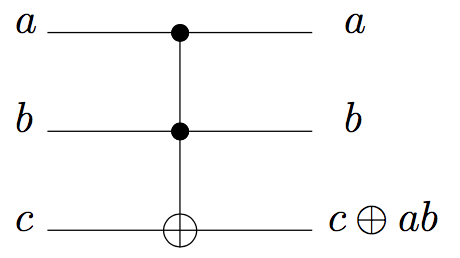
\includegraphics[width=1.5in]{images/toffoli.png}
\caption{Representation of the Toffoli gate.}
\label{toffoliGate}
\end{center}
\end{figure}

The reversibility of this operation is easily verified by observing that by applying the Toffoli door twice in a row the same starting result is obtained:
$$(a, b, c) \rightarrow{} (a, b, c \otimes ab) \rightarrow{} (a, b, c)$$

So the operation itself coincides with its inverse. It is equally easy to verify that the Toffoli gate represents the permutation $\pi = (67)$ on integers $0, 1, \ldots , 7$ (exchanges the two sequences $110$ and $111$).

Toffoli's door is universal for the classic reversible computations, that is, every classical computation can be built in a reversible way through the Toffoli door. This result follows from the universality of the operations of \texttt{NAND} and \texttt{FANOUT} (the operation of copying a classic bit) for the classical computations and from the fact that both these operations can be expressed through the Toffoli circuit. In fact, by applying the operation with $c = 1$, we obtain $a^{'}= a$, $b^{'} = b$ and $c^{'} = 1 \oplus ab = \neg ab$, i.e. the simulation of \texttt{NAND} as a reversible operation. The reversible \texttt{FANOUT} is instead obtained as shown in \autoref{fanoutToffoli}: by applying the Toffoli gate with $a = 1$ and $c = 0$ the result is the copy of bit $b$ (We remind you that this copy operation is not possible for a qubit).

\begin{figure}[!htb]
\begin{center}
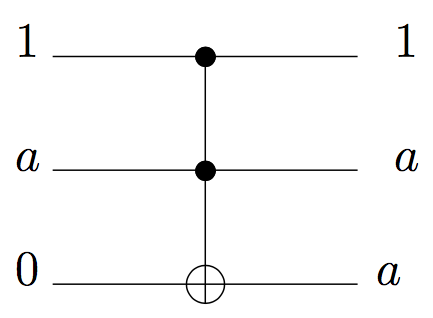
\includegraphics[width=1.5in]{images/fanoutToffoli.png}
\caption{FANOUT made through the Toffoli gate.}
\label{fanoutToffoli}
\end{center}
\end{figure}

As for \texttt{NAND} and \texttt{FANOUT} the construction of a reversible circuit for any classical operation $f$ by means of the Toffoli port involves the use of some service bits in input (or \textit{ancilla bits}) and in output (or \textit{garbage}). After deleting these service bits, the resulting circuit performs the transformation:
$$(x, y) \mapsto (x, y \otimes f(x))$$

(where $x$ is the input of $f$ and $y$ is the register intended to contain the output) and can be considered as the \textit{standard reversible circuit} for the evaluation of $f$.

\subsection{Classical computations on quantum circuits}

\paragraph{} As we have already observed, a classical reversible computation corresponds to a permutation on the sequences of the input bits. This guarantees the possibility of constructing a complex unitary matrix that represents it\footnote{A result of the theory of groups and representations ensures that there exists a representation, called the \textit{standard unitary representation}, of the symmetric group of the permutations on $2^{n}$ symbols in the group of complex unit matrices $2^{n}\times2^{n}$. This representation associates to a permutation $\pi$ the matrix $U$ of generic element $U_{ij} = \delta_i, \pi(j)$, where $\delta_{kl}$ denotes the Kronecker's delta defined so $\delta_{kl} = 1$ if $k = l$ and $\delta_{kl} = 0$ otherwise.}. In particular, the Toffoli door can be implemented as quantum circuit. In this case the input is given by three qubits and the transformation, analogous to the classical case, consists in the exchange of the third qubit if the first two are $1$. For example the quantum Toffoli gate applied to the state $|110\rangle$ produces the state $|111\rangle$. A simple exercise is to write the unitary matrix $U$ corresponding to this permutation.
The quantum Toffoli port can then be used to simulate all the classical computations on a quantum computer, ensuring that a quantum computer is able to perform any computable computation on a classic computer.

\subsection{Probabilistic computations on quantum circuits}

\paragraph{} \textit{Randomized} algorithms are algorithms that are executed using a random number generator (the launch of a coin) to decide one of the possible branches of execution. The first randomized algorithm was introduced by Solovay and Strassen in the 1970s to determine whether a number is prime or not. The algorithm produces a correct answer only with a certain probability. This probability can be increased by repeating the execution for an appropriate number of times.

These algorithms can also be efficiently simulated by quantum circuits. In fact, to simulate a random bit it is sufficient to prepare a qubit in the $|0\rangle$ state and then apply the Hadamard port. You will get the status $\frac{|0\rangle + |1\rangle}{\sqrt{2}}$ that measured will give $0$ or $1$ each with probability $1/2$. It should also be noted that in this way a ``really" random number is obtained, something that a classic computer can not do.

\section{Quantum parallelism}

\paragraph{} On a quantum computer, a function $f(x)$ can be evaluated on different values of $x$ at the same time. This is known as \textbf{quantum parallelism} and is a fundamental characteristic of quantum circuits.

Consider a boolean function of the form:
$$f : \{0, 1\} \mapsto \{0, 1\}$$

To calculate $f(x)$ by means of a quantum computation the transformation $f(x)$ must be defined as a unit transformation $U_f$. As seen previously, this can be done by applying on the input state $|x,y\rangle$, said data register, an appropriate sequence of quantum logic gates (which we will indicate with a black box called $U_f$) that transform $|x,y\rangle$ into the state $|x,y\rangle \oplus f(x)\rangle$, called the target register. If $y = 0$ then the final state of the second qubit will accurately contain the value of $f(x)$.

\begin{figure}[!htb]
\begin{center}
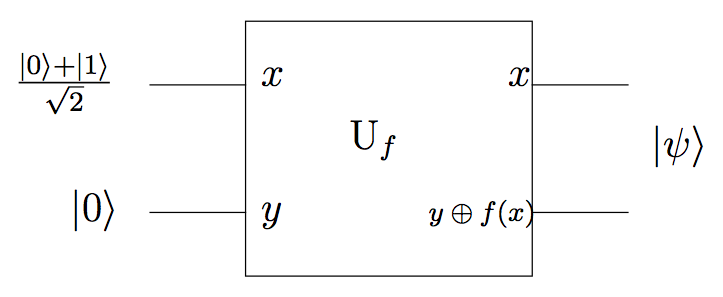
\includegraphics[width=1.5in]{images/qParal.png}
\caption{Quantum circuit to evaluate $f(0)$ and $f(1)$ simultaneously.}
\label{qParal}
\end{center}
\end{figure}

In the circuit in \autoref{qParal}, the input is
$$\frac{|0\rangle + |1\rangle}{\sqrt{2}} \otimes |0\rangle$$

that is, the value of $x$ is an overlap of $0$ and $1$ that can be obtained by applying Hadamard to $|0\rangle$. Applying $U_f$ to this data register is obtained
$$\frac{|0, f(0)\rangle + |1, f(1)\rangle}{\sqrt{2}}$$

This state contains information both on the value $f(0)$ and on the value $f(1)$. We then evaluated $f$ simultaneously on $x$ = 0 and $x = 1$. This type of parallelism is different from the classical one where multiple circuits (each of which calculates $f(x)$ for a single value of $x$) are executed simultaneously.

This procedure can be generalized to calculate functions on an arbitrary number of bits using a generalization of the Hadamard gate known as the \textbf{Walsh-Hadamard} transform. This operation consists of $n$ Hadamard ports acting in parallel on $n$ qubits. For example, for $n = 2$, the Walsh-Hadamard transform is indicated with $H^{\otimes 2} = H \otimes H$ and applied to two qubits prepared in the state $|0\rangle$ gives as a result
$$\frac{|0\rangle + |1\rangle}{\sqrt{2}} \otimes \frac{|0\rangle + |1\rangle}{\sqrt{2}} = \frac{|00\rangle + |01\rangle + |10\rangle + |11\rangle}{2}$$

In general, the result of $H^{\otimes n}$ applied to $n$ qubits in the $|0\rangle$ state is:
$$\frac{1}{\sqrt{2^n}}\sum\limits_{x}|x\rangle$$

where $x$ is the binary representation of the numbers from $0$ to $2^n - 1$. Thus, the Walsh-Hadamard transform produces an equiprobable overlap of all the states of the $n$ qubit computational basis. We observe that to obtain an overlap of $2^n$ states only $n$ logical ports are needed.

\paragraph{Exercise} Look exercises number 21 and 22 in \autoref{exs}.

The parallel evaluation of a function, $f(x)$ with input $x$ of $n$ bits and $1$ bit as output, can therefore be performed by a circuit similar to the one in Figure 17, with $n+1$ qubit in input prepared in the $|0\rangle^{\otimes n}|0\rangle$. Then Hadamard applies to the first $n$ qubits and then the $U_f$ circuit. The result will be
$$\sqrt{1}{\sqrt{2}}\sum\limits_{x}|x\rangle|f(x)\rangle$$

Quantum parallelism is not directly usable in the sense that it is not possible to obtain all the values calculated with a single measurement: the measurement of the state $\sqrt{1}{\sqrt{2}}\sum\limits_{x}|x\rangle|f(x)\rangle$ will give the value of $f(x)$ for a single value of $x$.

To exploit the hidden information in this parallelism, we have to, somehow, make better use of the information contained in the overlap $\sqrt{1}{\sqrt{2}}\sum\limits_{x}|x\rangle|f(x)\rangle$, for example by exploiting in an appropriate manner the interference between the states in the overlap. By combining quantum parallelism with this property that comes from quantum mechanics, results like the one exemplified by the Deutsch algorithm can be obtained.



\newpage

\section{Exercises}
\label{exs}
\paragraph{} In this section there are the exercises and the answers to them. 
\subsection{Questions}
\paragraph{Exercise 1}
\label{ex01q}
Extend the definitions and properties given for $\mathbb{R}^2$ to $\mathbb{R}^d, d \in \mathbb{N}$.

\paragraph{Exercise 2}
\label{ex02q}
Write the computational bases for a 3-qubit and 4-qubit quantum register.
\paragraph{Exercise 3}
\label{ex03q}
Demonstrate the bilinearity property:
\begin{equation*}
\begin{split}
(\alpha v + {\alpha}^{'} v^{'}) \otimes (\beta w + {\beta}^{'} w^{'}) = \\
\alpha \beta v \otimes w + \alpha {\beta}^{'} v \otimes w^{'} + {\alpha}^{'} \beta v^{'} \otimes w + {\alpha}^{'} {\beta}^{'} v^{'} \otimes w^{'} \\
\end{split}
\end{equation*}
where $\alpha, \beta, {\alpha}^{'}, {\beta}^{'} \in \mathbb{C}, v, v^{'} \in \mathbb{C}^k, w, w^{'} \in \mathbb{C}^l$.
\paragraph{Exercise 4}
\label{ex04q}
Demonstrate that:
$$\beta_{i}^{k} \otimes \beta_{l}^{j} = \beta_{(i-1)(l+j)}^{kl}$$.
\paragraph{Exercise 5}
\label{ex05q}
Demonstrate that: 
\begin{equation*}
\begin{split}
\forall \; \; v, v^{'} \in \mathbb{C}^{k}, w, w^{'} \in \mathbb{C}^{l} \\
\langle v \otimes w\rangle | v^{'} \otimes w^{'} = \langle v | v^{'}\rangle \langle w | w^{'}\rangle
\end{split}
\end{equation*}
\paragraph{Exercise 6}
\label{ex06q}
Demonstrate that:
\begin{enumerate}
    \item $$(M \otimes N) (v \otimes w) = (Mv)\otimes(Nw)$$
    \item
    \begin{equation*}
    \begin{split}
    (\alpha M + \alpha^{'} M^{'}) \otimes (\beta N + \beta^{'} N^{'}) = \\
    \alpha \beta M \otimes N + \alpha \beta^{'} M \otimes N^{'} + \alpha^{'} \beta M^{'} \otimes N + \alpha^{'} \beta^{'} M^{'} \otimes N^{'}
    \end{split}
    \end{equation*}
    \item $$(M \otimes N) (M^{'} \otimes N^{'}) = (MM^{'})\otimes(NN^{'})$$
    \item
    \begin{equation*}
    \begin{split}
    (M \otimes N)^{*} = M^{*} \otimes N^{*} \\
    (M \otimes N)^{T} = M^{T} \otimes N^{T} \\
    (M \otimes N)^{\dagger} = M^{\dagger} \otimes N^{\dagger} \end{split}
    \end{equation*}
    \item If $M$ and $N$ are unitary (invertible), then also $M \otimes N$ is unitary (invertible)
\end{enumerate}
\paragraph{Exercise 7}
\label{ex07q}
Demonstrate that the state $|00\rangle + |11\rangle$ can not be factored into the tensor product of two independent qubits, i.e. there is no $a_1, a_2, b_1, b_2$ such that $|00\rangle + |11\rangle = (a_1 |0\rangle + b_1 |1\rangle) \otimes (a_2 |0\rangle + b_2 |1\rangle$).
\paragraph{Exercise 8}
\label{ex08q}
Prove that the sum of two linear functions is linear.
\paragraph{Exercise 9}
\label{ex09q}
Prove that the linear function $|\psi\rangle\langle\phi| : \mathbb{C}^2 \mapsto \mathbb{C}^2$ defined from $|\psi\rangle\langle\phi|(|x\rangle) = \langle\phi|x\rangle|\psi\rangle$ is linear.
\paragraph{Exercise 10}
\label{ex10q}
Consider the base formed by the two qubits $|+\rangle = \frac{|0\rangle + |1\rangle}{\sqrt{2}}$ and $|-\rangle = \frac{|0\rangle - |1\rangle}{\sqrt{2}}$. The base change matrix from $|0\rangle$, $|1\rangle$ to $|+\rangle$, $|-\rangle$ is given by
\begin{equation*}
\begin{aligned}
B = \frac{1}{\sqrt{2}}
{\begin{bmatrix}
1 & 1 \\
1 & -1 \\
\end{bmatrix}}
\end{aligned}
\end{equation*}

\paragraph{Exercise 11}
\label{ex11q}
Verify that the representation of $L$ in the new base is $BAB^{-1}$.

\paragraph{Exercise 12}
\label{ex12q}
Prove that the representation of \texttt{NOT} in base $|0\rangle$ and $|1\rangle$ is the matrix
\begin{equation*}
\begin{aligned}
X = {\begin{bmatrix}
0 & 1 \\
1 & 0 \\
\end{bmatrix}}
\end{aligned}
\end{equation*}
What is its representation in the base $|+\rangle, |-\rangle$?
\paragraph{Exercise 13}
\label{ex13q}
Demonstrate that the Pauli matrices are unitary.
\paragraph{Exercise 14}
\label{ex14q}
Prove that $\langle u|A v \rangle = \langle A\dagger u | v \rangle$. Deduct the following property of the unit matrices: $M$ is unitary if and only if it preserves the scalar products, i.e. if and only if $\langle Mu|Mv \rangle = \langle u|v \rangle$, for each $u, v \in \mathbb{C}^2$.
\paragraph{Exercise 15}
\label{ex15q}
Demonstrate that linear function transforms a qubit into a qubit (that is, it preserves normalized vectors) if and only if it is unitary.
\paragraph{Exercise 16}
\label{ex16q}
Demonstrate that for each unitary matrix $U$ there are real numbers $\alpha, \beta, \delta, \gamma$ such that:
$$U = \begin{bmatrix}
e^{i(\alpha - \frac{\beta}{2} - \frac{\delta}{2})}cos(\frac{\gamma}{2}) & -e^{i(\alpha - \frac{\beta}{2} + \frac{\delta}{2})}sin(\frac{\gamma}{2}) \\
e^{i(\alpha + \frac{\beta}{2} - \frac{\delta}{2})}sin(\frac{\gamma}{2}) & e^{i(\alpha + \frac{\beta}{2} + \frac{\delta}{2})}cos(\frac{\gamma}{2})
\end{bmatrix}$$
\paragraph{Exercise 17}
\label{ex17q}
Consider a similar operation to the \texttt{CNOT} where the target is denied if the control qubit is zero rather than one. This operation is represented as in Fig. \ref{cnotvar}. What is the matrix that represents it?
\begin{figure}[!htb]
\begin{center}
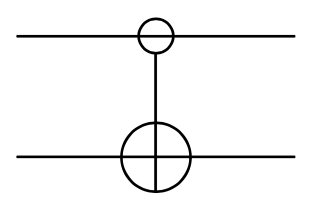
\includegraphics[width=1.0in]{images/cnotvar.png}
\caption{A different \texttt{CNOT} gate.}
\label{cnotvar}
\end{center}
\end{figure}
\paragraph{Exercise 18}
\label{ex18q}
Given a two-qubit system, demonstrate that the mean value of the observable $X_1Z_2$ measured in the state $(|00\rangle + |11\rangle)/\sqrt{2}$ is zero. The notation $X_1$ and $Z_2$ indicates respectively the Pauli $X$ operator applied to the first qubit and the Pauli $Z$ operator applied to the second qubit. 
\paragraph{Exercise 19}
\label{ex19q}
Consider the following status of a two-qubit register
$$|\psi\rangle = \frac{|00\rangle + |11\rangle}{\sqrt{2}}$$
Prove that there are no states $|a\rangle$ and $|b\rangle$ of the two qubits components such that $|\psi\rangle = |a\rangle|b\rangle$. 
\paragraph{Exercise 20}
\label{ex20q}
Verify that Bob can determine the two bits through measurements on a single qubit. (Hint: measure the second qubit and apply Hadamard to the first qubit of the resulting state).
\paragraph{Exercise 21}
\label{ex21q}
Demonstrate that:
$$H^{\otimes n} |0\rangle^{\otimes n} = \frac{1}{\sqrt{2}^n}\sum\limits_{x \in \{0, 1\}^{n}}|x\rangle$$
\paragraph{Exercise 22}
\label{ex22q}
Demonstrate that:
$$H|x\rangle = \frac{1}{\sqrt{2}}\sum\limits_{y \in \{0, 1\}}(-1)^{xy}|y\rangle$$
$$H^{\otimes n}|x\rangle = \frac{1}{\sqrt{2}^n}\sum\limits_{y \in \{0, 1\}^n}(-1)^{x \cdot y}|y\rangle$$
where $x \in \{0, 1\}^n$ and $x \cdot y$ is $\sum\limits_{j=1}^{n} x_iy_i \; \; module \; \; 2$
\paragraph{Exercise 23}
\label{ex23q}
Verify that the function defined by
$$((y_1, y_2, \ldots, y_n), (z_1, z_2, \ldots, z_n)) = \sum\limits_{i = 1}^{n}y_{i}^{*}z_i$$
where $(y_1, y_2, \ldots, y_n)$ and $(z_1, z_2, \ldots, z_n)$ are vectors in $\mathbb{C}^n$, it is an internal product.
\paragraph{Exercise 24}
\label{ex24q}
Find eigenvectors, eigenvalues and diagonal representation of Pauli matrices
\begin{equation*}
\begin{aligned}
X = \begin{bmatrix}
0 & 1 \\
1 & 0 \\
\end{bmatrix} \; \; \; 
Y = \begin{bmatrix}
0 & i \\
-i & 0 \\
\end{bmatrix} \; \; \;
Z = \begin{bmatrix}
1 & 0 \\
0 & -1 \\
\end{bmatrix}
\end{aligned}
\end{equation*}
\paragraph{Exercise 25}
\label{ex25q}
Show that the eigenvalues of a unit matrix all have module $1$ and therefore can be written in the form $e^{i\theta}$ with $\theta \in \mathbb{R}$.
\paragraph{Exercise 26}
\label{ex26q}
Show that the matrices of Pauli are Hermitian and unitary.
















\newpage

\subsection{Answers}
\paragraph{Exercise 1} 
\label{ex01a}
The $n$-dimensional real vector space ${\mathbb{R}}^n$ is the set of column vectors of the form
\begin{equation*}
\begin{aligned}
v = {\begin{bmatrix}
a_1 \\
\vdots \\
a_n
\end{bmatrix}}
\end{aligned}
\end{equation*}

where $\{a_1, \ldots, a_n\} \in \mathbb{R}$ are real numbers. 

The \textbf{norm} of $v$ is given by $|v| = \sqrt{a_1^2 +, \ldots, + a_n^2}$. 

The \textbf{transposed} of $v$ is the vector line $v^T = (a_1, \ldots, a_n)$. 

The \textbf{scalar product} of two vectors
$$v_a = {\begin{bmatrix}
a_1 \\
\vdots \\
a_n
\end{bmatrix}}, v_b = {\begin{bmatrix}
b_1 \\
\vdots \\
b_n
\end{bmatrix}}$$

is given by 
$$v_a \cdot v_b \stackrel{\text{def}}{\equiv} v_a^Tv_b = (a_1, \ldots, a_n) (b_1, \ldots, b_n)^T = a_1 b_1 +, \ldots, + a_n b_n = \norm{v_a}\norm{v_b}cos{\theta}$$

where ${\theta}$ is the angle between $v_a$ and $v_b$. If $v_a \cdot v_b = 0$, then the two vectors are \textbf{orthogonal}.

The vectors ${v_i \in {\mathbb{R}} \; | \; i = 1, 2,\ldots k}$ are called \textbf{linearly independent} if
$$a_1v_1 + a_2v_2 + \ldots + a_kv_k = 0, \; \; a_i \in {\mathbb{R}}$$

This implies that $a_i = 0$ for each $i = 1, 2, \ldots, k$. Otherwise they are called \textbf{linearly dependent}.

A \textbf{basis} of ${\mathbb{R}}^n$ is any set of linearly independent vectors such that any other vector in ${\mathbb{R}}^n$ can be expressed as a linear combination of the vectors in the set. Each set of $v_1, \ldots, v_n$ of linearly independent vectors form a base for ${\mathbb{R}}^n$. Further, $v_1, \ldots, v_n$ form an \textbf{orthonormal basis} for ${\mathbb{R}}^n$ if $\norm{v_1} \ldots \norm{v_n} = 1$ \textbf{and} $v_1 \cdot \ldots \cdot v_n = 0$. 
Consequently, the $n$ vectors
$$v_1 = {\begin{bmatrix}
v_{1,1} \\
\vdots \\
v_{1,n}
\end{bmatrix}}, \ldots, v_n = {\begin{bmatrix}
v_{n,1} \\
\vdots \\
v_{n,n}
\end{bmatrix}}$$

form an orthonormal basis for ${\mathbb{R}}^n$ called the \textbf{standard base} of ${\mathbb{R}}^n$.

\paragraph{Exercise 2}
\label{ex02a}
Standard computational basis for a three and four bits register are, respectively, 
$$|000\rangle, |001\rangle, |010\rangle, |011\rangle, |100\rangle, |101\rangle, |110\rangle, |111\rangle$$
and 
\begin{equation*}
\begin{split} 
|0000\rangle, |0001\rangle, |0010\rangle, |0011\rangle, \\ 0100\rangle, |0101\rangle, |0110\rangle, |0111\rangle, \\
1000\rangle, |1001\rangle, |1010\rangle, |1011\rangle, \\
1100\rangle, |1101\rangle, |1110\rangle, |1111\rangle
\end{split}
\end{equation*}
In vectorial form
\begin{equation*}
\begin{aligned}
{\begin{bmatrix}
1 \\
0 \\
0 \\
0 \\
0 \\
0 \\
\end{bmatrix}}
{\begin{bmatrix}
0 \\
1 \\
0 \\
0 \\
0 \\
0 \\
\end{bmatrix}}
{\begin{bmatrix}
0 \\
0 \\
1 \\
0 \\
0 \\
0 \\
\end{bmatrix}}
{\begin{bmatrix}
0 \\
0 \\
0 \\
1 \\
0 \\
0 \\
\end{bmatrix}}
{\begin{bmatrix}
0 \\
0 \\
0 \\
0 \\
1 \\
0 \\
\end{bmatrix}}
{\begin{bmatrix}
0 \\
0 \\
0 \\
0 \\
0 \\
1 \\
\end{bmatrix}}
\end{aligned}
\end{equation*}
and
\begin{equation*}
\begin{aligned}
{\begin{bmatrix}
1 \\
0 \\
0 \\
0 \\
0 \\
0 \\
0 \\
0 \\
\end{bmatrix}}
{\begin{bmatrix}
0 \\
1 \\
0 \\
0 \\
0 \\
0 \\
0 \\
0 \\
\end{bmatrix}}
{\begin{bmatrix}
0 \\
0 \\
1 \\
0 \\
0 \\
0 \\
0 \\
0 \\
\end{bmatrix}}
{\begin{bmatrix}
0 \\
0 \\
0 \\
1 \\
0 \\
0 \\
0 \\
0 \\
\end{bmatrix}}
{\begin{bmatrix}
0 \\
0 \\
0 \\
0 \\
1 \\
0 \\
0 \\
0 \\
\end{bmatrix}}
{\begin{bmatrix}
0 \\
0 \\
0 \\
0 \\
0 \\
1 \\
0 \\
0 \\
\end{bmatrix}}
{\begin{bmatrix}
0 \\
0 \\
0 \\
0 \\
0 \\
0 \\
1 \\
0 \\
\end{bmatrix}}
{\begin{bmatrix}
0 \\
0 \\
0 \\
0 \\
0 \\
0 \\
0 \\
1 \\
\end{bmatrix}}
\end{aligned}
\end{equation*}

\paragraph{Exercise 3}
\label{ex03a}
\paragraph{Exercise 4}
\label{ex04a}
\paragraph{Exercise 5}
\label{ex05a}
\paragraph{Exercise 6}
\label{ex06a}
\paragraph{Exercise 7}
\label{ex07a}
\paragraph{Exercise 8}
\label{ex08a}
\paragraph{Exercise 9}
\label{ex09a}
\paragraph{Exercise 10}
\label{ex10a}
\paragraph{Exercise 11}
\label{ex11a}
\paragraph{Exercise 12}
\label{ex12a}
\paragraph{Exercise 13}
\label{ex13a}
\paragraph{Exercise 14}
\label{ex14a}
\paragraph{Exercise 15}
\label{ex15a}
\paragraph{Exercise 16}
\label{ex16a}
\paragraph{Exercise 17}
\label{ex17a}
\paragraph{Exercise 18}
\label{ex18a}
\paragraph{Exercise 19}
\label{ex19a}
\paragraph{Exercise 20}
\label{ex20a}
\paragraph{Exercise 21}
\label{ex21a}
\paragraph{Exercise 22}
\label{ex22a}
\paragraph{Exercise 23}
\label{ex23a}
\paragraph{Exercise 24}
\label{ex24a}
\paragraph{Exercise 25}
\label{ex25a}
\paragraph{Exercise 26}
\label{ex26a}


\bibliographystyle{plain}
\bibliography{ref}

\section*{Notes}

\paragraph{}
\begin{enumerate}
    \item \url{https://www.youtube.com/watch?v=5xW49CzjhgI&feature=youtu.be}
\end{enumerate}

\end{document}